% Stanford University PhD thesis style -- modifications to the report style
% This is unofficial so you should always double check against the
% Registrar's office rules
% See http://library.stanford.edu/research/bibliography-management/latex-and-bibtex
% 
% Example of use below
% See the suthesis-2e.sty file for documentation
%
\documentclass{report}
\usepackage{suthesis-2e}
\usepackage{atlas-defs}
\usepackage{useful}
\usepackage{amsfonts} 

\usepackage{tabularx}


\usepackage{tikz}
\usepackage{wrapfig}
\usepackage{soul}
\usepackage{adjustbox}

\dept{Physics}

%%%%%%%%%%%%%%%%%%%%
% Some latex setup
%%%%%%%%%%%%%%%%%%%%
\newcommand*{\ATLASLATEXPATH}{latex/}

\usepackage[hepparticle,hepprocess]{\ATLASLATEXPATH atlasphysics}

\usepackage[biblatex=true,backend=bibtex]{\ATLASLATEXPATH atlaspackage}
\usepackage{\ATLASLATEXPATH atlasbiblatex}
\usepackage{\ATLASLATEXPATH atlasphysics}

% Files with references for use with biblatex.
% Note that biber gives an error if it finds empty bib files.
\addbibresource{thesis.bib}
\addbibresource{bib/ATLAS.bib}
\addbibresource{bib/CMS.bib}
\addbibresource{bib/ConfNotes.bib}
\addbibresource{bib/PubNotes.bib}
\addbibresource{bib/ATLAS-useful.bib}

% Some colors we're using for templates for fonts that it's fun to match for the note
\definecolor{hh:darkpink}{HTML}{f2385a}
\definecolor{hh:medturquoise}{HTML}{36b1bf}
\definecolor{hh:darkblue}{HTML}{343844}
\definecolor{hh:darkgreen}{HTML}{125125}
\definecolor{hdbs:outrageousorange}{HTML}{fa7e61}
\definecolor{rebeccapurple}{HTML}{663399}


\begin{document}

\title{Two b, and then another two b... but how to MLearn it bbbbest -- that's the question.}
\author{Nicole Hartman}
\principaladviser{Su Dong}
\firstreader{Michael Kagan}
\secondreader{Patricia Burchat}
\thirdreader{Michael Peskin} 
 
%\beforepreface
%
%\prefacesection{Preface}

There's something special about the human race that drives us not just to exist but to understand the reason for our existence.
A part of the mechanistic answer to this question comes from a desire to understand what are the fundamental building blocks of nature. 
As we moved away from the earth, fire, air, water understanding of the fundamental elements to a more modular undersanding of matter's components, in 400 BC, Democritus thought that he "had" it with the "elements" and he coined the word ``atoms'' to describe what we now understand as the periodic table of the elements.
Atom means ``uncuttable'' a now hilarious misnomer - as the systematic structure of the periodic table hinted at some underlying components, and the experimentally verified when Thomas X saw the electrons popping off of the atom and we came to understand the 
The evolution / progression of the scientific revolution has involved us studying ever smaller and smaller distance scales... and discovering a microcosm ever more and more intricate and facinating.
In my PhD, I've been working at SLAC the momentous institute where the substructure of the proton was discovered, a discovery which cemented our current understanding of the parton model and the Standard Model of particle phyiscs.
We keep reusing the word "elements" "elementary" because we are striving to get to these fundamental distance scales... 

Something absolutely facinating to me is the range of masses that we have in the SM that we understand to be entirely pointlike.
We currently believe that both the top quark 175 GeV  down to the < meV neutrino are entirely point-like objects, and it seems absolutely fascinating to me this 9 decade range of energies can similarly be packed into an infinitesimally small distance.
The Higgs is the answer to this mass generation - and therefore studying it and it's properties gives us a clue to this mystery.

This thesis submission marks a decade since the Higgs boson discovery, and we expect to observe the HH process in another 10 years of LHC data taking.
And although the Higgs mechaanism is now an old theory, with the massively large datasets we're collecting at the LHC, we can unlock new ways of answering these questions with the big data developments in the burgeoning field of deep learning.
This thesis explores the properties of the Higgs through the lens of the Run 2 dataset in this journey of understanding the microscopic realm -- a quest that continues to remain interesting, for a whole new generation of scientists to uncover and as we continue to ask the question... what will be next.
%\prefacesection{Acknowledgments}

\begin{chapquote}{Bill Burnett \& Dave Evans, \emph{Designing Your Life}.}
{Every domain of human endeavor is held together by a web of relationships between people. Real people. That web is the fabric that undergirds, contains, and holds together that part of society.}
\end{chapquote}

%\begin{chapquote}{Charles Dickens, \emph{A Tale of Two Cities}}
%{It was the best of times, it was the worst of times, it was the age of wisdom, it was the age of foolishness, it was the epoch of belief, it was the epoch of incredulity, it was the season of light, it was the season of darkness, it was the spring of hope, it was the winter of despair.}
%\end{chapquote}

I would like to thank...

\begin{itemize}
	\item Michael
	\item Rafael
	\item Max Swiatlowski
	\item HH->4b squad: Dale Abott, Sean G, Lukas Borgna 
	\item Other NR analyzers: James Grundy, Rui Zhang,
	\item FTAG / CP people: C Pollard, Franscesco de Bello, Jonathan Shalomi, Manuel Guth, Bing, Dan Guest, Binbin
	\item Danny Antrim, Kathryn, Johan, Matthew Feickert
	\item Steve, Jodi, Richard Scaletter, Emily Thompson
	\item Aviv
	\item Stats help: Lukas, Giordan
	\item Valentina and PF
	\item Jannicke
	\item SLAC ATLAS mentors: Caterina, Aeriel, Su Dong, Charlie
	\item Katharine + Liza: Making the best ATLAS sub-group in the world (supposedly a cult)
	\item HH Party planning committee
	\item HHonorable mentions: First tequila shot (CV) second tequila shot (MK)
	\item Amazing group collaborators: Maxime and Yoann
	\item Reading / exam committee
\end{itemize}

%
%\afterpreface
%
%\chapter{Introduction}
\begin{chapquote}{Thomas Khun, \emph{The Structure of Scientific Revolutions}}{Until taught by prolonged exposure that the universe contained anomalous cards, they saw only the types of cards for which previous experience had equipped them. Yet once experience had provided the requisite additional categories, they were able to see all anomalous cards on the first inspection long enough to permit any identification at all \ldots}
\end{chapquote}


\begin{itemize}
	\item Why we expect new physics in the SM
	\item Motivation for HH
	\item Particulars about the 4b final state
	\item Connection to ML
	\item Highlight my work on b-tagging
	\item Thesis organization
\end{itemize}


\textbf{Refs: }
\begin{itemize}
\item Higgs discovery:  \cite{HIGG-2012-27, CMS-HIG-12-028}.
\end{itemize}
%\chapter{Theoretical motivation}

\section{The Standard Model}

\section{The Higgs mechanism}
I heard from Dale that the pdg is a v good ref for this!!

\section{Effective Field Theories to search for new physics}

\section{Status of the experimental HH results}

%\chapter{The Large Hadron Collider}
\label{ch:lhc}
\begin{chapquote}{Pablo Picasso}
{Every act of creation begins with an act of destruction.}
\end{chapquote}


The LHC is a 27~km circumference particle accelerator straddling the border between France and Switzerland \cite{LHC}. It now collides bunches of $10^9$ protons every 25~ns at a center of mass energy of 13~TeV \cite{ATLAS_long}.
Bunches of protons are used since the proton radius is about 1~fm, and thus the probability of a head-on collision between single protons is increased by increasing the number of colliding particles.  We expect about 20 collisions per given bunch crossing at the LHC \cite{PU}.

Since the proton is not an elementary particle, but rather a baryonic resonant QCD bound state, even a head-on collision will not have all of the available energy concentrated at a point.
The proton is a composite particle made up of two up and one down valence quarks, along with a sea of virtual quarks and gluons that spontaneously come out of the vacuum because of the uncertainty relation $\Delta x \Delta p \geq \hbar / 2$.  
The 6.5~TeV per proton is distributed among these partons\footnote[3]{A parton is a constituent of a hadron.}.  Therefore, to look at the high-energy regime, we are interested in a ``hard scatter'' where a single quark or gluon carrying a large fraction of one proton's momentum collides with a high energy constituent of the other proton, lending to the production of one or more Higgs bosons.

\begin{itemize}
	\item History
	\item Collider Stats
	\item I should make a set of slides (or app) making sure that I know what the dipole and focusing magnets do!!
\end{itemize}

\begin{figure}[hbt]
\centering
\subfloat[]{\includegraphics[width=.45\textwidth]{{figures/lhc/intlumivstimeRun2DQall.pdf}}}
\subfloat[]{
	\includegraphics[width=.45\textwidth]{{figures/lhc/mu_2015_2018.pdf}}
	\label{PU density profile for Run~2 data taking.}
	}
\caption{Need to cite: https://twiki.cern.ch/twiki/bin/view/AtlasPublic/LuminosityPublicResultsRun2\#Pileup\_Interactions\_and\_Data\_Tak}
\end{figure}
%\chapter{The  ATLAS detector}
\label{ch:atlas}
\begin{chapquote}{Lorde ``Yellow Flicker Beat''}
{I never watch the stars -- there's so much down here.}
\end{chapquote}



\def\figpath{figures/Undergrad thesis/}

\newcommand{\AtlasCoordFootnote}{ATLAS uses a right-handed coordinate system with its origin at the nominal interaction point
in the centre of the detector and the \(z\)-axis along the beam pipe.
The \(x\)-axis points from the interaction point to the centre of the LHC ring,
and the \(y\)-axis points upwards.
Cylindrical coordinates \((r,\phi)\) are used in the transverse plane, 
\(\phi\) being the azimuthal angle around the \(z\)-axis.
The pseudorapidity is defined in terms of the polar angle \(\theta\) as \(\eta = -\ln \tan(\theta/2)\).
Angular distance is measured in units of \(\Delta R \equiv \sqrt{(\Delta\eta)^{2} + (\Delta\phi)^{2}}\).}

%-------------------------------------------------------------------------------
\section{Overview}
%-------------------------------------------------------------------------------

%%% default ATLAS stuff

The ATLAS detector~\cite{PERF-2007-01} at the LHC covers nearly the entire solid angle around the collision point.\footnote{\AtlasCoordFootnote}
It consists of an inner tracking detector surrounded by a thin superconducting solenoid, electromagnetic and hadronic calorimeters,
and a muon spectrometer incorporating three large superconducting toroidal magnets.
The inner detector system (ID) is immersed in a \SI{2}{\tesla} axial magnetic field 
and provides charged-particle tracking in the range \(|\eta| < 2.5\).
The high-granularity silicon pixel detector covers the vertex region and typically provides four measurements per track, 
the first hit being normally in the insertable B-layer (IBL) installed before Run~2~\cite{ATLAS-TDR-2010-19,PIX-2018-001}.
It is followed by the silicon microstrip tracker (SCT) which usually provides eight measurements per track.
These silicon detectors are complemented by the transition radiation tracker (TRT),
which enables radially extended track reconstruction up to \(|\eta| = 2.0\).\footnote{Text taken from the ATLAS approved detectors text section of the repo, but I'm just including the tracker info since I use hits as my variables.} 
%%% end of default ATLAS stuff

A cutaway view of the ATLAS detector is shown in \Fig{ATLAS-detector}.  The inner detector (ID) provides charged particle tracking information closer to the interaction point.  The inner detector is immersed in a 2~T solenoidal magnetic field to bend the trajectories of charged particles and allow for momentum measurement. 
\begin{figure}[h!tbp]
\centering
\includegraphics[width = \textwidth]{{\figpath/ATLAS_detector.png}}
\caption{Cut away of the ATLAS detector
~\cite{ATLAS_long}}
\label{ATLAS-detector}
\end{figure}
Energy measurement is made in two parts: with an electromagnetic and hadronic calorimeter.  Finally, the outermost layer of the detector is the muon spectrometer, with a 4~T toroidal magnetic field. 

\subsection{ATLAS Coordinate System}

At the ATLAS detector, the z-axis is measured along the accelerator beam pipe, the x-axis points into the center of the ring, and y-axis is defined to point vertically up by the properties of a right-handed rectilinear coordinate system.  
Then a cylindrical coordinate system is used for the ATLAS detector.
The azimuthal angle, $\phi = \arctan(\frac{y}{x})$, denotes orientation in the plane transverse to the beam, and the pseudorapidity, $\eta$, measures the polar angle inside the detector, where
%
\begin{equation}
\eta = -\ln \left( \tan \left(\frac{\theta}{2} \right) \right)
\end{equation}
%
and where $\theta \in [0,\pi]$ is the polar angle as measured from the z-axis.  The ATLAS detector is forward-backward symmetric to maximize the detector coverage since colliding protons each have the same energy.

From these detector variables, we can get components in the four-momentum using the relations %(derivation shown in Ref~\cite{eta_phi_Cartesian}).
\begin{equation}
(E,p_x, p_y, p_z) = (E,p_T \cos \phi, p_T \sin \phi,p_T \sinh \eta)
\label{momentum-conversion1}
\end{equation}
\begin{equation}
p = p_T \cosh \eta
\label{momentum-conversion2}
\end{equation}
We can also get a measurement of the momentum in the calorimeter for relativistic particles.  In the relativistic limit, the energy and momentum are the same (in natural units).  However, when the momentum is defined from a calorimeter measurement, $E_T$ is used instead of $p_T$. Equations~\eqref{momentum-conversion1} and \eqref{momentum-conversion2} still apply in this case.

\clearpage

\section{Tracker}

\subsection{Inner Detector}
\label{inner_detector}

A cutaway view of the inner detector for ATLAS is shown in \Fig{ATLAS-InnerDetector}.
\begin{figure}[h!tbp]
\centering
\includegraphics[scale=0.9]{\figpath/ATLAS_inner_detector.png}
\caption{Illustration of the orientation of the subsystems inside the ATLAS Inner Detector~\cite{Aad:2008Jinst}}
\label{ATLAS-InnerDetector}
\end{figure}

\begin{figure}[h!tbp]
\centering
\includegraphics[width = \textwidth]{\figpath/ID_table.png}
\caption{List of the dimensions of the subsystems in the ID~\cite{ATLAS_long}.}
\label{ID-table}
\end{figure}
With approximately 1000 tracks emerging from the interaction point every 25~ns, the ID is divided into three different regions to optimize the pattern recognition and momentum measurement algorithms \cite{ATLAS_long}.  
The pixel detectors have the most precision, so this layer is closest to the interaction point. The pixel detector also has the highest cost, so the next least expensive tracking option is the silicon microstrip trackers (SCTs), at the next farthest region away from the interaction point.  Finally, the Transition Radiation Trackers (TRTs) compose the outermost region of the inner detector.
The ID uses pattern recognition to measure transverse momentum as low as 0.5~GeV, and provides electron identification for $|\eta| < 2.0$ for energies up to 150~GeV \cite{ATLAS_long}. Displaced multi-particle vertexes can be resolved by the pixel detector and help identify long-lived B-hadrons.

\begin{figure}[h!tbp]
\centering
\includegraphics[width = \textwidth]{\figpath/ID_color.png}
\caption{The structural elements in the ID at $\eta = 0.3$~\cite{ATLAS_long}.}
\label{ID_color}
\end{figure}

\begin{figure}[h!tbp]
\centering
\includegraphics[width = \textwidth]{\figpath/ID_endcap.png}
\caption{The structural elements in the ID at $\eta = 1.4$~\cite{ATLAS_long}.}
\label{ID_endcap}
\end{figure}

\clearpage
\begin{wrapfigure}{r}{0.45\textwidth}
\centering
\includegraphics[width=0.4\textwidth]{\figpath/Pixel_cartoon.png}
\caption{Schematic for the general idea for how a pixel detector tracks incident particles.
~\cite{Quantum_diaries}}
\label{Pixel-cartoon}
\end{wrapfigure}

\subsubsection{Pixel Tracking System}

ATLAS is often referred to as a ``giant camera.''  
In a general sense, both a camera and the ATLAS detector provide ways to record specific events, but the parallels run deeper than their purposes, since both cameras and particle detectors can obtain information via pixels.  In a camera, an incident photon will go through a silicon diode and knock a valence electron free to generate a few electron-hole pairs.  An electric field is set up across the pixel and will then pull the electron and hole apart to the metal contacts where the charge can be read out \cite{Quantum_diaries}.  The pixel detector at ATLAS works in a similar way, except the energy of the incident particles at ATLAS is orders of magnitude larger: while a photon of visible light has an energy of a few eV, typical ``interesting'' particles at the LHC are in the MeV to TeV range.  

As a particle passes through the pixel sensor, it creates electron-hole pairs that are separated by the electric field and read out by the electronics, as shown in \Fig{Pixel-cartoon}. 

The pixel sensors in ATLAS consist of 80 million \cite{Detector_challenges} rectangular $50~\mu$m$ \times 400~\mu$m ``n$^+$-in-n'' electrodes.\footnote{The ``n'' region is n-type, or  doped with atoms that are electron donors; the ``in'' region is intrinsic, or undoped; and the ``n$^+$'' region is also n-type, but doped more heavily than other n region.}
The pixel detector's position with respect to the other components of the inner detector is shown in \Fig{ATLAS-InnerDetector}. 
Zooming in on  \Fig{ATLAS-InnerDetector}, the innermost part of the inner detector---the pixel detector---is shown in \Fig{ATLAS-PixelDetector}.  The 80 million channels are divided into four cylindrical layers combined in a volume 1442 mm in length with 430 mm radius \cite{Aad:2008Jinst}. The pixel detector has a resolution of 15 microns, and this precision is limited by the size of the electronics.

\begin{figure}[h!tbp]
\centering
\includegraphics[scale=0.9]{\figpath/ATLAS_pixel_detector.png}
\caption{Illustration of the active region of the pixel detector with the barrel and endcap layers~\cite{Aad:2008Jinst}}
\label{ATLAS-PixelDetector}
\end{figure}

The pixel detector starts 5~cm from the center of the beam pipe to gain as much information about the central reaction as possible, and has coverage for $|\eta| < 2.5$~\cite{Detector_challenges}.
Since the pixel detector is so close to the interaction point, its electronics must be able to withstand high radiation doses of up to 500~kGy.  The p-n diodes can experience a leakage current when an electron-hole pair has enough energy to overcome the potential barrier.  
The detector minimizes the number of electron-hole pairs spontaneously generated by cooling the system at $-6^\circ$C.

\subsubsection{Silicon Microstrip Trackers}
The Silicon Microstrip Trackers (SCTs) operate with a similar principle as the pixel detectors, but have an effective operating voltage determined by the effective doping level, and their leakage current also increases linearly with radiation dose.
Initially the operating voltage was 150~V, but increased up to 250 to 350~V to compensate for the radiation dose after 10~years.
The 15912 SCT sensors each have a thickness of $285\pm15~\mu$m and a pitch of $80~\mu$m.
%(See p58 of ATLAS long for more details)

\subsubsection{Transition Radiation Tracker}
\label{trt}

The Transition Radiation Trackers (TRT) make up the outermost region of the ID, and the dimensions of the TRT are shown in \Fig{ID-table}.  ``Transition Radiation'' is the radiation emitted by a relativistic particle as it traverses an interface between two materials with different permittivities.
Each TRT is a 4~mm polyimide drift tube, created by two 35~$\mu$m multi-layer films bonded back-to-back \cite{ATLAS_long}.  
A 25~$\mu$m thick polyimide film has one side laminated with a 0.2 $\mu$m of Al with another 5-6~$\mu$m layer of graphite \cite{ATLAS_long}. 
The inside of the tube is filled with a gas composed of 70\%~Xe, 27\%~CO$_2$, and 3\%~O$_2$. 
The anode is composed of 31~$\mu$m diameter cylinder of tungsten wire positioned at the center of the drift tube, and coated with 0.5--0.7~$\mu$m of gold.
After fabrication, the tubes were cut to a 144~cm length for the barrel and 37~cm length for the end-cap region.  
The barrel straws are read out at each end of the tube, so the middle of the tube is insulated with a 6~mm glass layer which creates a 2~cm spot where the element is not sensitive to incident tracks.
The anode is grounded and connected to the front end electronics, while the cathodes are held at $-1530$V.  Minimizing mechanical sag in the straw is crucial for accounting for the error in the position measurements, so the straws are mechanically supported by carbon fibers \cite{ATLAS_long}.

\begin{figure}[h!tbp]
\centering
\includegraphics[width=\textwidth]{\figpath/TRT_cartoon.png}
\caption{Principle of operation for the TRT~\cite{TRT}}
\label{GEANT_sim}
\end{figure}

An incident particle traversing a straw ionizes the gas molecules to free electrons and positive ions.  The electrons accelerate through the electric field to the anode, and these electrons in turn will ionize other ions to create a gain of $2.5\times10^4$.  Since the anode is read out at both ends of the wire, this provides a drift time measurement from the difference of arrival times between the two ends of the wire.  The time resolution is approximately a nanosecond, which corresponds to a spatial resolution of about 100~microns.  

An outgoing particle will hit on average 36 of the TRT tubes; this improves the momentum measurement in the inner detector.
During its lifetime, a straw detector can track $10^{15}$ particles, and a total integrated charge of 1000~C, which corresponds to about 20~years of the LHC's operation.  
The ATLAS inner detector has 12,000 of these straws in the endcaps and 52,544 straws in the barrel, yielding a total of 351,000 read--out channels.  Although the silicon trackers need to be cooled between $-5$ to $-10^\circ$C, the TRTs operate at room temperature.



\section{Calorimeter}

\subsection{ECAL}

Calorimetry literally means ``heat measurement.'' The incident particle interacts with the material in the detector to form a shower of particles which are decelerated and absorbed in the detector material to reconstruct the original particle's energy.  
The ATLAS calorimeter is divided into two parts: the electromagnetic calorimeter (ECAL) and the hadronic calorimeter (HCAL).  The ECAL is for electromagnetic interactions and has higher precision than the HCAL which reconstructs the particles interacting by the strong force.   

\subsubsection{Sampling vs. Homogenous Calorimeters}

For an electromagnetic shower to develop, incident electrons (and positrons) will emit a photon through Bremsstrahlung approximately in through a distance characterized by the radiation length
\begin{equation}
X_0=\frac{716.4~{\text{g}} \cdot {\text{cm}}^{-2}  A}{Z(Z+1) \ln{ \frac{ 287 }{ \sqrt{Z} }}}
\label{radiation_length}
\end{equation}
where $A$ is the number of nucleons and $Z$ is the atomic number (number of protons) in the detector material~\cite{Calorimetry1}.
The units of $X_0$ means that dividing by the density gives the actual distance traveled by a particle \cite{Calorimetry2}.
Then the photons will in turn pair-produce electrons and positrons when traveling a distance of $\frac{9}{7} X_0$.  This showering phenomena will continue until the average particle energy decreases to below the critical energy, $E_c=\frac{610~{\text{MeV}}}{Z+1.24}$.
The hadronic showers are characterized by the interaction length, $\lambda = 37.8 A^{0.312} {\text{g}} \cdot {\text{cm}}^{-2}$, the average distance that an incident particle travels before undergoing a nuclear interaction.  

\begin{wrapfigure}{r}{0.5\textwidth}
\centering
\includegraphics[width=0.45\textwidth]{\figpath/Sampling_Cal.png}
\caption{Schematic illustrating how a sampling calorimeter causes an incident particle to form a shower more quickly.
~\cite{Sampling_Cal}}
\label{sampling-schematic}
%\vspace*{-5mm}
\end{wrapfigure}

Two different calorimeter designs can be used to measure the incident particle's energy.  In a sampling calorimeter, the volume is divided into scattering and absorbing slabs, shown in \Fig{sampling-schematic}.  
The scattering slabs use a high Z material to decrease the radiation length and allow the shower to develop more quickly.  
The energy deposited in the absorbing region of the calorimeter is measured, and the total energy is the energy deposited in the absorbing region divided by a scale factor, $f_{sampling}= E_{visible} / E_{deposited}$.   A sampling calorimeter contains the shower in a smaller detector to help minimize the cost of the experiment.  
One of the downsides of this procedure is that the sampling method is not as precise because only a fraction of the energy deposited is measured, and fluctuations proportional to $\sqrt{E}$ for Poisson statistics will introduce extra errors into the measurements.

A homogenous calorimeter circumvents this problem by using the whole calorimeter as an active volume.  
A homogenous calorimeter is only useful as an ECAL since hadronic interactions require more material to ``contain,'' and it may not be monetarily feasible to construct such a large volume.  
To see this, we can look at the approximate formulas for the radiation length and interaction length, $X_0\sim \frac{A}{Z^2}$ , and $\lambda \sim A^{1/3}$. Since Z is approximately $\frac{1}{2} A$, this means  $\frac{\lambda}{X_0} \sim A^{4/3}$, a number that can be as large as 30 for high Z materials such as lead, showing that hadronic showers have a larger extent.  

\subsubsection{Liquid Argon Detector}
The ATLAS ECAL is a sampling calorimeter arranged in an accordion structure, as shown in \Fig{accordian-structure}.  The high Z material (Z = 82) lead creates the shower, while the energy is measured in liquid argon (LAr), a low Z material (Z = 18).  
As illustrated in \Fig{accordian-structure}, the folding angle decreases as the  radius (measured out from the interaction point) increases.  The folding angle varies between $90^\circ$ and $67^\circ$ to keep the LAr sampling region width approximately constant at 2.1mm between the absorbers.

\begin{figure}[h!tbp]
\centering
\includegraphics[width=\textwidth]{\figpath/accordian_structure.png}
\caption{Accordian sampling structure for calorimeter.
~\cite{LAr}}
\label{accordian-structure}
\end{figure}

The LAr scintillators are read out with wavelength-shifting photosensors.   
This type of a detector lends itself naturally to a tower structure with the modules forming wedges pointing back to the interaction point, shown in \Fig{Wedge-LAR-accordian}. This makes it easy for a particle's shower to be contained within a few modules or cells.  The segmentation in $\Delta \eta \times \Delta \phi$ is $0.025 \times 0.1$ in the pre-sampler region, $0.0031 \times 0.1$ in the strips, $0.25 \times 0.25$ in the main region, and $0.5 \times 0.025$ in the back region. This yields an energy resolution of 10-12\% GeV$^{-1/2}$.   

\begin{figure}[h!tbp]
\centering
\includegraphics[scale=0.5]{\figpath/Wedge_LAR_accordian.png}
\caption{Wedge showing the accordian structure for the liquid Argon portion of the calorimeter.
~\cite{LAr}}
\label{Wedge_LAR_accordian}
\end{figure}

\subsection{HCAL}

The hadronic calorimeter (HCAL) is the layer just outside of the ECAL, and measures the 
energy of hadrons that traverse the ECAL without stopping, as well as minimum-ionizing particles like muons.
Although the ECAL system could be used to measure the development of the hadronic showers as well, the HCAL system's coarser granularity decreases the monetary cost in covering this larger volume.  It is divided into three parts: the tile calorimeter, the LAr hadronic end--cap calorimeter, and the LAr forward calorimeter, as shown in \Fig{calorimeter}.

\begin{figure}[h!tbp]
\centering
\includegraphics[width=\textwidth]{\figpath/calorimeter.png}
\caption{Calorimeter system at ATLAS~\cite{ATLAS_long}.}
\label{calorimeter}
\end{figure}

\subsubsection{Tile Calorimeter}
The tile calorimeter is just outside ECAL and has an inner radius of 2.28~m and an outer radius 4.45~m.  
The barrel covers $|\eta| < 1.0$, while the extended barrels cover $0.8 < |\eta| < 1.7$.
It is a sampling calorimeter with a steel absorber and scintillating tiles read out with wavelength shifting fibers and photomultiplier tubes. 
Azimuthally divided into 64 modules, the barrel is segmented into three regions at $1.5\lambda, 1.8\lambda$, and $4.25\lambda$, while the extended barrel has $1.5\lambda, 2.6\lambda$, and $3.3\lambda$ depth segmentation.
At $\eta = 0$, the HCAL has a 9.7$\lambda$ depth \cite{ATLAS_long}.

\subsubsection{LAr hadronic end--cap calorimeter}
The LAr hadronic end--cap calorimeter has two wheels per endcap just behind the ECAL endcap calorimeter and housed within the same LAr cryrostats.
The wheels have two depth segments, 25~mm parallel copper plates for the wheels closest to the interaction point, and 50~mm plates for the wheels farther from the interaction point.  The wheels are divided into 32 wedges, with inner and outer radii of 0.475m and 2.03m, respectively.  The copper plates are filled with LAr as the active sampling volume \cite{ATLAS_long}.

\subsubsection{LAr forward calorimeter}
The forward calorimeter covers $\eta >3.1$ and is approximately 10 interaction lengths deep.
Each side has three modules, the first of copper  for electronic measurements, and the second two of tungsten for hadronic measurements.



\section{Muon system}

\subsection{Muon Spectrometer}

%\subsubsection{Motivation}
The tracking system determines the transverse momentum of a charged particle from its radius of curvature in a magnetic field since $R = p_T /(qB)$.  A more massive object moving at the same velocity will have a larger transverse momentum, and therefore a larger radius of curvature.  Since the muon is 200 times heavier than an electron, it can be difficult to have a tracking system that can accurately measure the momentum for relativistic muons and electrons, so the muon detection system is distinct to measure the $p_T$ for a broad range of muon energies.  

The muon detector is a gas detector like the TRT, and operates according to similar principles. 
The subsections below detail the components of the muon spectrometer, while the parameters for the coverage and number of channels for are listed in \Fig{Muon-table}.

\begin{figure}[h!tbp]
\centering
\includegraphics[width=0.75\textwidth]{\figpath/Muon_table.png}
\caption{Main parameters for the Muon Spectrometer.  The values in parentheses refer to the configuration from 2009~\cite{ATLAS_long}.}
\label{Muon-table}
\end{figure}

\subsubsection{Toroidal Magnets}

The muons are detected through the deflection of their tracks in a 4~T magnetic field.  There are three large air--core toroids, and each of these 3 toroids has 8 coils.  
The particles of interest that reach this portion of the detector are muons and neutrinos, but only the muons will be detected because the electrically neutral neutrinos are not deflected by the magnetic field.  
Backgrounds for the muon spectrometer are photons and neutrons with energies below an MeV and 100~MeV, respectively \cite{ATLAS_long}.  
The magnetic field is designed to be transverse to the muons' flight direction to minimize multiple scattering. The magnets are housed within cryostats to keep them below the critical temperature for superconductivity.  Inside these magnets are the muon chambers divided into three cylindrical chambers about the beam axis in the barrel region, while the transition and end--cap regions arranged as disks, also divided into three chambers \cite{ATLAS_long}.

\subsubsection{Monitored Drift Tubes}

The Monitored Drift Tubes (MDTs) are drift chambers that provide precision measurements. Each tube is made of aluminum with a 3~cm diameter and length between 0.9 and 6.2~m.  
The tube is filled with a 93\%~Ar,~7\%~CO$_2$ gas mixture, at a pressure of 3-bar \cite{ATLAS_long}.  It has a gain of $2\times10^4$ \cite{ATLAS_long}, similar to the TRT drift chambers (see \Section{trt}). The precision for single muon events is 100~$\mu$m, while the precision for multi-muon events is 50~$\mu$m \cite{ATLAS_long}. To control the precision, the sag of the wires is minimized by three kinematical mounts placed strategically to minimize distortion due to the support, as shown in \Fig{MDT-alignment}. There are a total of 1174 MDTs positioned in the barrel of the ATLAS detector ($|\eta| < 2$).

\begin{figure}[h!tbp]
	\centering
	\subfloat[Illustration of how an MDT works ~\cite{ATLAS_long}.]{
	\includegraphics[width=0.25\textwidth]{\figpath/MDT_cartoon.png}
	\label{MDT_cartoon}
	}
	\subfloat[The orientation of the multi-layer MDT chamber with the support structure~\cite{ATLAS_long}.]{
	\includegraphics[[width=0.65\textwidth]{\figpath/MDT-alignment.png}
	\label{MDT_alignment}
	}
\caption{Monitored Drift Tubes: MDTs}
\end{figure}

\subsection{Cathode Strip Chambers}
\label{cdc}
For larger pseudorapidities ($2 < |\eta| < 2.7$), Cathode Strip Chambers (CSCs) are used for their higher granularity in the endcap region \cite{ATLAS_long}.  This is a multi-wire proportional chamber with strip read--out with a sense wire pitch of 2.54~mm and a read--out strip pitch of 5.08~mm resulting in a 60~$\mu$m track resolution \cite{ATLAS_long}.  


\FloatBarrier
\clearpage
\section{Trigger system}
\label{sec:atlas-trigger}

The LHC collides proton bunches 40~million times each second -- but the vast majority of these events don't contain interesting physics. Since it is infeasible to record every proton-proton collision, ATLAS utilizes a two stage of trigger that determine which events to save and write to disk \cite{ATLAS_long}, with an overview in \Fig{\ref{fig:trig-latency}}.  

\begin{figure}[h]
\centering
\includegraphics[width=\textwidth]{figures/atlas/trig-latency-graphic}
\caption{Illustration of the data acquisition chain -- a sequence of decisions in hardware (L1) and software (HLT) which determines which events get saved \cite{javier-iaifi-2} \cite{ATL-COM-DAQ-2014-054}.}
\label{fig:trig-latency}
\end{figure}

The first stage is the Level I (L1) trigger takes a very coarse view of the detector and has a $\mu s$ to decide whether to keep the event. This prohibits computationally expensive algorithms (such as tracking) being run, so L1 only looks at trigger objects using information from the calorimeter and muon systems.
Since these algorithms need to be very fast, they're implemented in hardware using field programmable gate arrays (FPGAs) before the electronic signals are read off of the detector.
It reduces the rate by almost three orders of magnitude (to 100 kHz) for sending the electronic signals off of the detector.
 

The second stage is High Level Trigger (HLT) is the software based trigger system, that implements an event reconstruction very similar to the offline algorithms. At this stage, tracking information is available, so \Pqb-tagging information can be used in the trigger decision (of particular importance for the HH $\rightarrow$ 4b analysis). 
There are several different ``trigger streams'' or combinations of selections applied to the trigger objects to collect datasets of interest to the diverse physics program.  Events passed from all of these trigger steams get saved at a rate of 1 kHz while data is being taken. 
%The estimate of the jet's energy is also much more accurate than it was at L1. 



%\begin{figure}
%\centering
%\includegraphics[width=.5\textwidth]{figures/atlas/dataset-sizes}
%\caption{\hl{If I include this, I'll have to find an original source to understand what everything means} \cite[javier-iaifi-2].}
%\label{fig:dataset-sizes}
%\end{figure}

%
%\chapter{Event Reconstruction}
\label{ch:evtReco}

\section{Overview}
(electrons, photos, muons, + taus)
I might mention them ... I might not b/c they aren't used by 4b
At least I should mention e- and muons tho...

\section{Tracks}

\section{Vertex reconstruction}

The event's selected primary vertex (PV) is defined as the reconstructed primary vertex with largest $\sum \pT^2$ of the associated tracks. 


\section{Jets}

\subsection{Jet clustering algorithms}

A given $pp$ collision produces many quarks and gluons.  However, because of the ``confinement principle,'' no free color charge can exist, which means no isolated quarks or gluons can exist in nature. %\cite{SM_Higgs, Particle_World}.  
It becomes energetically favorable for quark / anti-quark pairs to pop out of the vacuum to balance the color charge imbalance by forming color neutral hadrons. 
This sparks a chain reaction which produces a spray of particles in the detector. 

The anti-k$_T$ algorithm provides a way to cluster the energy deposited in the calorimeter to form a ``jet,'' and is the standard algorithm for defining jets at ATLAS \cite{antiKt}.  First it defines two quantities, 
%
\begin{equation}
d_{ij} = {\text{min}}( p_{Ti}^{-2}, p_{Tj}^{-2}) \frac{\Delta R_{ij}}{R^2} \qquad \qquad  d_i = p_{Ti}^{-2}
\end{equation}
%
where $\Delta R_{ij}^2 = (y_i - y_j)^2 + (\phi_i - \phi_j)^2$, and $R$ is the jet-radius, defined by the user.  To find the jets, the algorithm
%
\begin{itemize}
\item{Calculates $d_{ij}$ and $d_i$ for all particles in the event, and lets $d$ be the smallest $d_i$, $d_{ij}$.}
%\item{Find all the $d_{ij}$ and $d_i$ in the event, and let $d = min(\{d_{ij}, D_i\})$}
	\begin{itemize}
	\item{If $d = d_{ij}$, then it combines jet $i$ and jet $j$.}
	\item{If $d = d_{i}$, then it lets jet $i$ be the final jet.}
	\end{itemize}
\item{It continues the previous steps until all the particles in the event have been accounted for.}
\end{itemize}
%
This algorithm clusters high-$p_T$ particles together if they fall within the jet's radius. \\

The $pp$ collisions at 13~TeV typically will give rise to about 20 moderate $p_T$ jets in the detector, or around ${{20}\choose{2}} = 190$ viable di-jet candates.  So the challenge in elucidating the $H\rightarrow b\bar{b}$ or $HH \rightarrow 4b$ signals is accurately finding the ``correct'' pair(s) of jets.

Since the protons are not point-like, the colliding partons may not have equal $p_T$ in the lab frame. By definition, the net momentum will be zero in the center of mass (CM) frame.  A heavy ($\sim$TeV) resonance can be created at (or nearly at) rest in the CM frame, but when Lorentz boosting back into the lab frame the decay products can become highly collimated.  When the decay products can no longer be resolved individually, we instead search for jets with a large radius parameter (``fat jets''), indicative of merged jets \cite{SM_Higgs, Merged_Jets}.  The constituent clusters inside a fat jet are called \emph{subjets}.  
Large R (about 1.0) correspond to fat jets, and R about 0.4 correspond to the standard resolved jets.


\subsection{PFlow}

\subsection{VR}

\subsection{Boosted jets}

\subsection{Muons}
Def useful for muon in jet + pt reco correction!!

%\subsection{Pileup suppression}
%\subsection{Event cleaning}
% I'm tempted to talk about these, but since they're not directly related 
% to the core contributions of my thesis work, I'm going to skip it.
% Oh - I should j add what I put in the int note!!


%\chapter{b-tagging}

\section{Low level taggers}

\subsection{IP2D and IP3D}

\subsubsection{Lifetime signage}

\begin{figure}[htbp]
  \centering
 \includegraphics[width=0.5\textwidth]{figures/ftag/lifetime-signage}
 \caption{Lifetime signage graphic (from \cite{giacinto-thesis})}
 \label{fig:lifetime-signage}
\end{figure}


\textbf{3d sign}

$\Delta \vec{r}_{IP} = \vec{r}_{IP}  - \vec{r}_{PV} $

\begin{equation}
  \text{sign}_{3D} =   \text{sign} \left( \left[ \vec{p}_{trk} \times \vec{p}_{jet} \right] \cdot \left[   \vec{p}_{trk} \times \Delta \vec{r}_{IP} \right] \right)
  %\label{eq:}
\end{equation}

\textbf{2d sign}

\begin{equation}
  \text{sign}_{r \phi} =   \text{sign} \left( \sin \left( \phi_{jet} - \phi_{trk} \right) \cdot d_{0,trk} \right)
  %\label{eq:}
\end{equation}

\begin{equation}
  \text{sign}_{z} =   \text{sign} \left(  \left(  \eta_{jet} - \eta_{trk} \right) \cdot z_{0,trk}  \right)
  %\label{eq:}
\end{equation}



(Equations taken from Giacinto's thesis  \cite{giacinto-thesis}.)

\textbf{How are the IPs signed for the IP2D and IP3D algorithms}

\begin{itemize}
	\item \textbf{IP2D: }
	\begin{itemize}
	\item$d_0$ signed based on the projection of the vectors in the (x,y) plane
	\end{itemize}

	\item \textbf{IP3D:}
	\begin{itemize}
	\item $d_0$ signed with the 3D vectors
	\item $z_0$ signed based on the $(r, \phi)$ plane
\end{itemize}
\end{itemize}

\subsubsection{Mathematical motivation}


\begin{figure}[htbp]
  \centering
 \includegraphics[width=0.5\textwidth]{figures/ftag/Naive-Bayes-illustration}
 \caption{Probabilistic graphical model illustration for a Naive Bayes algorithm.  }
  \label{fig:Naive-Bayes-illustration}
\end{figure}

%%%%%%%%%%%%%%%%%%%%%%%%%%%%
% Plot showing the non-independence of the tracking inputs
%%%%%%%%%%%%%%%%%%%%%%%%%%%%

%\def\figpath{figures/ftag/ATL-PHYS-PUB-2017-003/}
\begin{figure}[htbp]
  \centering
  \subfloat[]{\includegraphics[width=0.5\textwidth]{figures/ftag/ATL-PHYS-PUB-2017-003/fig_01a}}
  \subfloat[]{\includegraphics[width=0.5\textwidth]{figures/ftag/ATL-PHYS-PUB-2017-003/fig_01b}}
  \caption{ \cite{ATL-PHYS-PUB-2017-003}}
  \label{fig:rnnip-note-trk-ind}
\end{figure}


\subsubsection{Algorithm description}

% I don't think I need to describe the benefit of IP based algorithms
%\textbf{Should I mention that the lifetime signage is different between IP2D and IP3D? No - beyond the scope!}


The IP3D algorithm \cite{FTAG-2018-01} assigns probabilities to tracks based on two-dimensional likelihood templates, with the tracks' $z_0\sin\theta$ and $d_0$ lifetime signed significances, built from simulated jets.
These templates are obtained in 14 exclusive categories defined by the hit patterns of the tracks, and separately for tracks in $b$-jets, $c$-jets and light-flavour jets. 
The inclusive distribution of $z_0\sin\theta$ and $d_0$ lifetime signed significances for the different jet flavours are shown in Figure \ref{fig:flippedInputs}.
% The IP3D algorithm builds histograms for estimating the likelihood distribution of the IP significance for the tracks in $b$-jets and $l$-jets in 14 exclusive categories defined by the hit patterns of the tracks \cite{FTAG-2018-01}. 
By assuming that the track probabilities inside a jet are independent, jet-level likelihoods can be constructed by multiplying the individual probabilities.
The IP3D $b$-tagging discriminants are therefore defined as:
\begin{equation}
D_{\text{IP3D,l}} = \log \prod_{i \in \text{tracks}} \frac{p_b^i}{p_l^{i}} \qquad D_{\text{IP3D,c}} = \log \prod_{i \in \text{tracks}} \frac{p_b^i}{p_c^{i}}.
\end{equation}
% multiplication over the track likelihoods produces a jet level probability, and the ratio of jet probabilities from the $l$ and $b$ hypotheses defines the $b$-tagging discriminant: $\log \prod_{i \in tracks} p_b^{(i)} / p_l^{(i)}$.
RNN based IP algorithms aim to overcome this overly simplistic assumption of independence, and offer the possibility to employ more features than only the IP significance in the discriminant~\cite{ATL-PHYS-PUB-2017-003}. 

%%%%%%%%%%%%%%%%%%%%%%%%%%%%
% Plot from the DIPS note
%%%%%%%%%%%%%%%%%%%%%%%%%%%%
\def\figpath{figures/ftag/dips-note/}
\begin{figure}[htbp]
  \centering
  \subfloat[]{\includegraphics[width=0.5\textwidth]{\figpath/sd0}}
  \subfloat[]{\includegraphics[width=0.5\textwidth]{\figpath/sz0}}
  \caption{Lifetime signed transverse (a) and longitudinal (b) significances for $b$-jets, $c$-jets and light-flavor jets.}
  \label{fig:flippedInputs}
\end{figure}

%%%%%%%%%%%%%%%%%%%%%%%%%%%%%%%%
% Table of the IPXD categories
%%%%%%%%%%%%%%%%%%%%%%%%%%%%%%%%

\begin{table}[h!]
  \begin{center}
    \begin{adjustbox}{width=\columnwidth,center}
    \begin{tabular}{ l | l | c c c  } % <-- Alignments: 1st 2 cols left, last three 3rd right, with vertical lines in between
      {} & {} &  \multicolumn{3}{ c }{ Fractional contribution [\%] } \\
      \textbf{\#} & \textbf{Category}  & \Pqb-jets & \Pqc-jets & light-jets  \\
      \midrule 
      0 & No hits in first two layers; expected hit in IBL and b-layer & 1.9 & 2.0 & 1.9   \\
      1 & No hits in first two layers; expected hit in IBL and no expected hit in b-layer & 0.1 & 0.1 & 0.1 \\
      2 & No hits in first two layers; no expected hit in IBL and expected hit in b-layer & 0.04 & 0.04 & 0.04 \\
      3 & No hits in first two layers; no expected hit in IBL and b-layer & 0.03 & 0.03 & 0.03 \\
      4 & No hit in IBL; expected hit in IBL & 2.4 & 2.3 & 2.1 \\
      5 & No hit in IBL; no expected hit in IBL & 1.0 & 1.0 & 0.9  \\
      6 & No hit in b-layer; expected hit in b-layer & 0.5 & 0.5 & 0.5 \\
      7 & No hit in b-layer; no expected hit in b-layer & 2.4 & 2.4 & 2.2  \\
      8 & \emph{Shared} hit in both IBL and b-layer & 0.01 & 0.01 & 0.03  \\
      9 & At least one \emph{shared} pixel hits & 2.0 & 1.7 & 1.5  \\
      10 & Two or more \emph{shared} SCT hits & 3.2 & 3.0 & 2.7  \\
      11 & \emph{Split} hits in both IBL and b-layer & 1.0 & 0.87 & 0.6  \\ 
      12 & \emph{Split} pixel hit & 1.8 & 1.4 & 0.9 \\
      13 & Good quality & 83.6 & 84.8 & 86.4 
    \end{tabular}
    \end{adjustbox}
    \caption{Categories for defining the IP2D and IP3D templates \cite{ATL-PHYS-PUB-2017-013}.}
    \label{table:IPXD-categories}
  \end{center}
\end{table}


\section{RNNIP}

\subsection{Algorithm overview}

\subsection{Optimizations}

\subsection{Interplay with tracking inputs}


\subsection{SV1}
\subsection{JetFitter}
\subsection{SMT}


\section{RNNIP}

\subsection{Algorithm overview}

\subsection{Optimizations}

\subsection{Interplay with tracking inputs}


\section{Recommendations for Run 2 b-taggers}

\subsection{DL1(r) description}

\subsection{PFlow trainings}

% link
% http://atlas.web.cern.ch/Atlas/GROUPS/PHYSICS/PLOTS/FTAG-2019-005/


\subsection{VR track jet trainings}

% link
% http://atlas.web.cern.ch/Atlas/GROUPS/PHYSICS/PLOTS/FTAG-2019-006/


\section{RNNIP calibratability}

\subsection{Calibration results}

\def\figpath{figures/ftag/DL1r-calibration}

\begin{figure}[htbp]
    \centering
    \subfloat[]{ 
            \includegraphics[width=0.48\linewidth]{\figpath/fig_01}
    } 
     \subfloat[]{ 
            \includegraphics[width=0.48\linewidth]{\figpath/fig_02}
    } 
    \caption{}
    \label{fig:pflow-calib}
\end{figure}

\subsection{Desiderata for a flipped tagger}


\begin{figure}[htbp]
  \centering
 \includegraphics[width=0.5\textwidth]{figures/ftag/fipped-tagger-graphic}
 \caption{Illustration of how the lifetime signage is less likely to be negative for a long lived particle (from Andy Buckley's slides).}
 \label{fig:lifetime-signage}
\end{figure}


\begin{figure}[htbp]
    \centering
    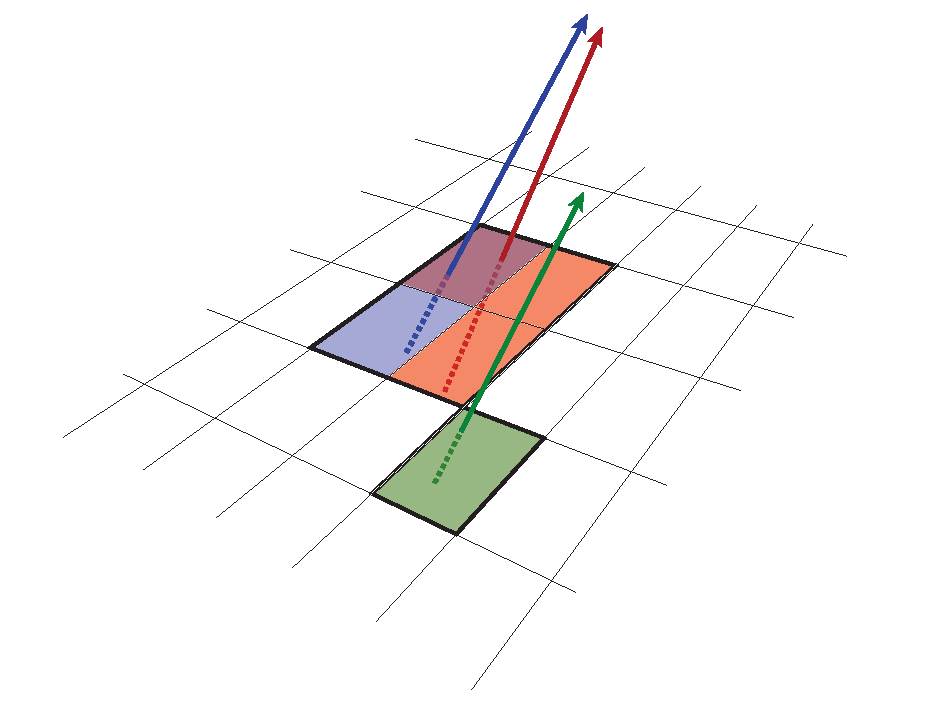
\includegraphics[width=0.8\linewidth]{\figpath/fig_03}
    \caption{}
    \label{fig:pflow-calib-light}
\end{figure}

\section{Tagger R\&D: DIPS}

%\input{Run 3 taggerrs}

%
%\chapter{Statistical techniques}
%
%\chapter{HH Physics overview}
\label{ch:hh-phys}
\def\figpath{figures/nr-int-note/intro/V1/}

\def\kl{$\kappa_\lambda$}

\section{HH signatures}

Probing the HH self-coupling is extremely interesting, but in the SM, the dominant gluon-gluon-fusion (ggF) cross-section is fantastically low at $\sigma_{ggF\,HH}^{\text{SM}} = 31.05$.\footnote{This includes next-next-to-leading order (NNLO) corrections with an the infinite top limit. The uncertainties  of $\sigma_{ggF\,HH}^{\text{SM}} = 31.05$ $\pm 3\%$ (PDF+$\alpha_{s}$) $^{+ 6\%}_{-23\%}$ (Scale + $m_{\text{top}}$)\,fb~\cite{Grazzini_2018} for a Higgs mass of 125 \GeV.}.
\hl{Could I give a rule of thumb for how much smaller this is c.f. other processes at the LHC?}

There are two diagrams that contribute to this process at leading order, as shown in \Fig{\ref{fig:ggF_feyn_dias}}, where there are two diagrams, the box diagram (\Fig{\ref{fig:ggF_feyn_dias}}) where the top loop radiates two Higgs bosons, and a triangle diagram (\Fig{\ref{fig:ggF_feyn_dias}}) which is includes the coupling of interest since the Higgs radiated by the top produces another two Higgses by its self-coupling. 
%In the SM, we see HH events 2000x less often than single Higgs events 
Although the process is so rare that we won't see it until the HL-LHC \cite{hh-proj}, we could see it sooner if the Higgs self-coupling deviates from the expectation. In the $\kappa$ framework, we parametrize the deviations of the couplings from the SM values, i.e, $\kappa_\lambda = \lambda / \lambda_{SM}$, and we can parametrize the deviations of the SM couplings from the other values similarly as well.

\begin{figure}[h]
    \centering
    \subfloat[The box diagram.]{
        \includegraphics[width=0.45\textwidth]{\figpath/ggF_box.pdf}
        \label{fig:boxFig{\ref{fig:ggF_feyn_dias}}}
    }
    \subfloat[The triangle diagram.]{
        \includegraphics[width=0.45\textwidth]{\figpath/ggF_tri.pdf}
        \label{fig:triangle}
    }
    \caption{The leading order gluon-gluon fusion di-Higgs production Feynman diagrams.}
    \label{fig:ggF_feyn_dias}
\end{figure}

In \Fig{\ref{fig:box_tri}}, you can see the contribution from each of the terms individually, and the interference between the two processes.
In the SM, this process is suppressed to destructive interference between these two diagrams.


\begin{figure}[h]
    \centering
    \includegraphics[width=0.8\textwidth]{figures/my_dihiggs/box_triangle_diagram.pdf}
    \caption{Impact of the interference of the box and triangle diagrams for ggF HH production.}
    \label{fig:box-tri}
\end{figure}



%%%%%%%%%%%%%%%%%%%%%%%%
%     VBF
%%%%%%%%%%%%%%%%%%%%%%%%

\textbf{from James - need to rephrase sentences}
The second-leading \HH production process is vector boson fusion (VBF), which has a SM cross-section over an order of magnitude smaller than ggF, at $\sigma_{VBF\,\HH}^{SM} = 1.726$ $\pm 2.1\%$ (PDF+$\alpha_{s}$) $^{+0.03\%}_{-0.04\%}$(Scale)\,fb~\cite{Dreyer_2018} at next-to-next-to-next-to-leading order (N3LO) for a SM Higgs boson with mass of 125 \GeV. 


\begin{figure}[t]
    \centering
    \subfloat[]{
        \includegraphics[width=0.33\textwidth]{\figpath/VBF_kvkl.pdf}
        \label{"fig:VBF_kvkl"}
    }
    \subfloat[]{
        \includegraphics[width=0.33\textwidth]{\figpath/VBF_k2v.pdf}
        \label{"fig:VBF_k2v"}
    }
    \subfloat[]{
        \includegraphics[width=0.33\textwidth]{\figpath/VBF_kvkv.pdf}
        \label{"fig:VBF_kvkv"}
    }
    \caption{The three tree-level vector boson fusion di-Higgs production Feynman diagrams.}
    \label{fig:VBF_feyn_dias}
\end{figure}

\begin{figure}
    \centering
    \includegraphics[width=0.7\textwidth]{\figpath/hhbr-dkpink}
    \caption{Branching ratios of the di-Higgs at the LHC.}
    \label{fig:branching-ratios}
\end{figure}

\begin{figure}
    \centering
    \includegraphics[width=0.7\textwidth]{figures/my_dihiggs/truth_mhh_ggf_common_presel.pdf}
    \caption{Impact of the destructive interference for the \kl variations.}
    \label{fig:truth-hh-presel}
\end{figure}


\section{Datasets and signal parametrization}

\begin{itemize}
	\item Explain why we don't want to generate every single signal
\end{itemize}

\subsection{ggF: histogram based reweighting}

\def\Eq{Eq.~{#1}}

\textbf{Math from my notes reading the 2018 HH comb paper}

Although \Fig{\ref{fig:ggF_feyn_dias}} shows the LO Feynman diagrams, there is a fully differential next-to-leading-order (NLO) calculation, but the terms in this calculation still break down into diagrams in the box and triangle families.
Denoting the sum of the terms in the box and triangle diagrams as $B$ and $T$, respectively.
The impact from a non-SM coupling factors comes as a multiplicative factor for the corresponding vertices, allowing us to write down a combined amplitude (parametrized by $\kappa_t$ and $ \kappa_\lambda$ as:

\begin{equation}
\mathcal{A}(\kappa_t, \kappa_\lambda) &= \kappa_t^2 B + \kappa_t \kappa_\lambda T .
\end{equation}


The ggF cross section is obtained by squaring the amplitude:

\begin{align}
	\sigma(pp \rightarrow HH) \sim |\mathcal{A}^2| = \left( \kappa_t^2 B^* + \kappa_t \kappa_\lambda T^* \right) \left( \kappa_t^2 B + \kappa_t \kappa_\lambda T \right)  \\
	= \kappa_t^4 \left[ |B|^2 + \frac{\kappa_\lambda}{\kappa_t} (B^* T + T^* B) + \left( \frac{\kappa_\lambda}{\kappa_t}  \right)^2 |T|^2 \right] .
	\label{eq:xsec-kl-kt}
\end{align}

The $\kappa_t^4$ term scales the rate of the process. The $2^{nd}$ order $\kappa_\lambda / \kappa_t $ polynomial dictates the way these diagrams interfere, so with 3 different \kl values, we can get any arbitrary \kl value.

To simulate full kinematic sample, consider the basis functions woth $\kappa_t = 1$ and $\kappa_\lambda = 0$ (no triangle diagram), $\kappa_\lambda =1$ and a final (now arbitrary) $\kappa_\lambda = 20$.
 
Plugging these basis points into \Eq{eq:xsec-kl-kt} we get three different differential cross-sections:
 
\begin{align}
|\mathcal{A}(1,0)|^2 &= |B|^2 \\
|\mathcal{A}(1,1)|^2 &= |B|^2 +  (B^* T + T^* B)  + |T|^2  \\
|\mathcal{A}(1,\kappa_0)|^2 &= |B|^2 +  \kappa_0 (B^* T + T^* B)  + \kappa_0^2 |T|^2  \\
\end{align}

\def\a{|\mathcal{A}(1,0)|^2}
\def\b{|\mathcal{A}(1,1)|^2}
\def\c{|\mathcal{A}(1,\kappa_0)|^2}

\def\x{|B|^2} 
\def\y{(B^* T + T^* B) }
\def\z{|T|^2}

Now we solve for $\x$, $\y$, and $\z$ as a function of $\a$, $\b$, and $\c$
Define $x = \x$, $y = \y$, $z=\z$ and $a = \a$, and write this more concisely as a system of linear equations: 

\begin{equation}
\begin{bmatrix} 
a \\ b \\ c
\end{bmatrix}
 = \begin{bmatrix} 
	1 & 0 & 0 \\
	1 & 1 & 1\\
	1 & \kappa_0 & \kappa_0^2 \\
\end{bmatrix}
\begin{bmatrix} 
x \\  y \\ z
\end{bmatrix}
\end{equation}

\begin{equation}
a = x
%
\qquad \text{and} \qquad
%
\begin{bmatrix} 
b - a \\ c-a
\end{bmatrix}
 = \begin{bmatrix} 
	1 & 1\\
	\kappa_0 & \kappa_0^2 \\
\end{bmatrix}
\begin{bmatrix} 
y \\ z
\end{bmatrix}
\end{equation}

Taking the inverse of the matrix to solve for the remaining two terms:

\begin{equation}
\begin{bmatrix} 
y \\ z
\end{bmatrix}
 = \frac{1}{\kappa_0 (\kappa_0 - 1)} \begin{bmatrix} 
	\kappa_0^2  & 1-\\
	-\kappa_0 & 1 \\
\end{bmatrix}
\begin{bmatrix} 
b-a \\ c-a
\end{bmatrix}
\end{equation}


\begin{align}
y &=  \frac{1}{\kappa_0 (\kappa_0 - 1)} \left[  \kappa_0^2 (b-a) - (c-a) \right]  &=  \\
z &=   \frac{1}{\kappa_0 (\kappa_0 - 1)} \left[ - \kappa_0 (b-a) - (c-a)  \right]  &= \\
\end{align}

\textbf{Histogram Reweighting}

We use $\kappa_t = 1$ and $\kappa_\lambda = 0, 1, and 20$.

\textbf{This is an empirical assumption that all of the event level kinematics are \textbf{captured} by the mHH variable!}

\hl{Oh - could I include my plot here instead of MH's?}

\subsection{VBF: event level reweighting}

\section{EFTs}

\section{7.3 Analysis optimization strategy}

\begin{figure}
    \centering
    \includegraphics[width=0.9 \textwidth]{figures/ATLAS-CONF-2021-052/fig_08.pdf}
    \caption{Impact of the HH channels in the combination for the resonant scalar mass $m_X$ search \cite{ATLAS-CONF-2021-052} .}
    \label{fig:truth-hh-presel}
\end{figure}


\begin{figure}[h]
    \centering
    \subfloat[SM]{
    \includegraphics[width=0.33\textwidth]{figures/my_dihiggs/truth_mhh_sm.pdf}
    }
    \subfloat[\kl = 2]{
    \includegraphics[width=0.33\textwidth]{figures/my_dihiggs/truth_mhh_kl_2.pdf}
    }
    \subfloat[\kl = 10]{
    \includegraphics[width=0.33\textwidth]{figures/my_dihiggs/truth_mhh_kl_10.pdf}
    }
    \caption{Impact of the NR analysis selection for selected ggF signals.}
    \label{fig:truth-hh-sel}
\end{figure}


\begin{itemize}
	\item{Show how the sensitivity for 4b is \emph{not as great} at low mass}
\end{itemize}

%\chapter{Analysis selection}
\label{ch:analysis}

\begin{figure}[hb]
	\centering
	\includegraphics[trim={0 5cm 0 3cm},clip,width=\textwidth]{{figures/my_dihiggs/analysis-overview-graphic.pdf}}
	\caption{Illustration of the high-level analysis strategy.}
	\label{fig:analysis-sel}
\end{figure}

\section{Triggers}

\def\figpath{figures/nr-int-note/trigger/V1/}

This analysis uses a combination of multi \Pqb-jet triggers. 
The \pt thresholds and \Pqb-tagging working points vary slightly by the year of data taking ( with the specific cut values delineated in \Tab{\ref{tab:nr-triggers}}).
note - only 2 \Pqb-tags are required in the trigger to avoid creating a bias in the control region used in the background estimation that will be described in \Sect{\ref{sec:rw-overview}}.
The \Pqb-tagging SFs are derived for each trigger chain individually required our analysis strategy to specify which trigger stream was considered for the trigger SF application.
One other interesting feature of our analysis is our signal is not fully efficient for our analysis, as illustrated by efficiencies that are less than 100\% in Fig{\ref{fig:HH_trigger_eff}}, and also this efficiency is varying as a function of the reconstructed 4-jet invariant mass. 
 
\begin{table}[htbp]
\centering
\begin{tabular}{p{2cm}  p{1cm} | p{6cm}  | p{4.5cm} }
\textbf{Trigger Type} & Year & HLT thresholds & L1 thresholds \\
\hline
{} & 2016 & \small{ $\pt > 100$~GeV jet \& two $\pt > 55$~GeV 60\%~WP \Pqb-jets } &  \small{ five $\pt > 15$~GeV jets} \\
\textbf{2b1j} & 2017 &  \small{ $\pt > 150$~GeV jet \& two $\pt > 55$~GeV 70\%~WP \Pqb-jets }&  \small{ $\pt > 85$~GeV jet \& two $\pt~>~30$~GeV jets } \\
{} & 2018 &  \small{ $\pt > 150$~GeV jet \& two $\pt > 55$~GeV 70\%~WP \Pqb-jets }&  \small{ $\pt > 85$~GeV jet \& two $\pt~>~30$~GeV jets }\\
\hline
{} & 2016 &  \small{ four $\pt > 35$~GeV jets, two 60\% WP \Pqb-tags} & {} \\ 
\textbf{2b2j} & 2017 &  \small{four  $\pt > 35$~GeV jets, two 40\% WP \Pqb-tags} &  \small{four $\pt > 15$~GeV,  $|\eta| < 2.5$ jets} \\
{} &  2018 &  \small{four $\pt > 35$~GeV jets, two 60\% WP \Pqb-tags}  & {} \\
\end{tabular}
\caption{Triggers used for non-resonant searches. For \Pqb-tagging in the trigger in Run 2, the MV2 version of the \Pqb-tagger is used. Also, an L1 $|\eta| < 3.2$ cut is assumed where not specified.}
\label{tab:nr-triggers}
\end{table}

\begin{figure}[htb]
        \centering
                \includegraphics[width=0.32\textwidth]{\figpath/SMNR_ggF_600043-2b1j-trigger-efficiency.pdf}
                \includegraphics[width=0.32\textwidth]{\figpath/SMNR_ggF_600043-2b2j-trigger-efficiency.pdf}
                \includegraphics[width=0.32\textwidth]{\figpath/SMNR_ggF_600043-2b1j+2b2j-trigger-efficiency.pdf}
        \caption{Trigger efficiencies of the 2b1j, 2b2j and combined for the MC16a/d/e corresponding to years 2016-2018 for the SM ggF \kl=1 signal.
        Significantly lower efficiency for 2017 2b2j comparing to other years is due to tighter b-tagging requirement (lower efficiency). \hl{Is this plot inside of the SR?}}
	\label{fig:HH_trigger_eff}
\end{figure}

To account for this feature of ``operating on the turn on curve'' the SF that we apply to account for the trigger effects 

%%%%%%%%%%%%%%%%%%%%%%%%%%%%%%%
\subsection{Trigger buckets}
%%%%%%%%%%%%%%%%%%%%%%%%%%%%%%%

To distinguish which trigger chain to check, we cut on the offline jets $p_{\text{T},1} > 170$~GeV and $p_{\text{T},3} > 70$~GeV, where the jets are ordered by \pt.
These jet \pt cuts mimic the 2b1j trigger.
If the event passes these jet cuts, we put it in trigger \textbf{bucket 1}, otherwise it goes in trigger \textbf{bucket 2}.
In trigger bucket 1, we check the decision of the 2b1j trigger to decide whether to keep the event, and in trigger bucket 2, we check the 2b2j trigger. This procedure is summarized graphically in \Fig{\ref{fig:trigger-bucket-strategy}}.

\begin{figure}[htbp]
    \centering
    \includegraphics[width=0.8\textwidth]{\figpath/nr_buckets_diagram_simple.pdf}
    \caption{Trigger bucket strategy for non-resonant searches.}
    \label{fig:trigger-bucket-strategy}
\end{figure}

\Fig{\ref{fig:trig-bucket-4b}} shows how this strategy of using a combination of two triggers gives us sensitivity to complementary phase spaces in the analysis. The 2b1j trigger drives our acceptance for the high \mhh events, while the 2b2j trigger provides our low \mhh acceptance.

\begin{figure}
    \centering
    \includegraphics[width=0.48\textwidth]{\figpath/buckets_comparison_4b_ggF_SM_SR.pdf}
    \includegraphics[width=0.48\textwidth]{\figpath/buckets_comparison_4b_VBF_SR.pdf}
    \caption{The bucket composition of \mhh for the SM ggF (left) and \kvv = 0 VBF (right) \HH MC simulation in the 4b Signal Regions.  Bucket 1 corresponds to the 2b1j trigger and Bucket 2 corresponds to the 2b2j trigger.}
    \label{fig:trig-bucket-4b}
\end{figure}

To reconstruct the trigger decision and define the jet level SFs, offline jets are matched to the online jets using a $\Delta R$matching criterion.
% There are different cuts being used:
% - dR < 0.4 for defining the trigger match and applying the CDI SFs
% - dR < 0.3 for deriving the HLT ET SFs
% - dR < 0.4 for deriving the L1 ET SFs
% but I'm not sure if dR < 0.4 is always used for applying these SFs
These online jets are then checked to pass the (online) thresholds given in Table~2, and if this many jets and \Pqb-jets pass this selection, the event passes this trigger. 
For ease of knowing how to apply the SFs, we will only keep events where the trigger passed in the relevant bucket, i.e, the 2b1j trigger needs to pass if the event passed the offline cuts in bucket 2, and the 2b2j trigger needs to pass if the event passed the offline cuts in bucket 1.
The event level trigger SF is calculated from the jet level SFs (\Eq{\ref{eq:trig-sf-all}}) with two contributions:

\begin{equation}
\text{Multi \Pqb-jet trigger SF} = \prod_i \textcolor{dodgerblue}{  SF_{jet}^{b-tag}(i)} \times \textcolor{orange}{SF_{jet}^{kinematic}(i)}  
\label{eq:trig-sf-all}
 \end{equation}

\begin{itemize}
\item \textcolor{dodgerblue}{ \Pqb-jet trigger SFs using prescription from by the \Pqb-jet trigger group (described in \Sect{\ref{subsec:trig-sf-bjet}})}
%(although they were customly rederived down to 30 GeV since we were investigating a low \pT category).}
\item  \textcolor{orange}{ Kinematic $E_\text{T}$ HLT and L1 SFs derived in a custom $t\bar{t}$ analysis (described in \Sect{\ref{subsec:trig-sf-et}})}
\end{itemize}

%%%%%%%%%%%%%%%%%%%%%%%%%%%%%%%
\subsection{b-jet SF}
\label{subsec:trig-sf-bjet}
%%%%%%%%%%%%%%%%%%%%%%%%%%%%%%%

The offline and online \Pqb-tagging decisions are highly correlated, so the online \Pqb-tagging SF are derived conditional based on the offline \Pqb-tagging decision. 
Since both the offline and online $\Pqb$-tagging decisions could pass or fail, this gives four cases:

\begin{itemize}
\setlength\itemsep{-1.5em}
   \item Case 1: Pass online and offline \Pqb-tagging: 
   	\vspace{-1em}
	  \begin{equation*}
		 \varepsilon(\text{on} \land \text{off}) 
		 = \varepsilon(\text{on} | \text{off}) \varepsilon(\text{off})
	  \end{equation*}
   \item Case 2: Fail the online \Pqb-tag, but pass the offline \Pqb-tag: 
   	\vspace{-1em}
	  \begin{equation*}
		 \varepsilon(\overline{\text{on}} \land \text{off}) 
		 = [1 - \varepsilon(\text{on} | \text{off})] \varepsilon(\text{off})
	  \end{equation*}
   \item Case 3: Pass the online \Pqb-tag, but fail the offline \Pqb-tag: 
   	\vspace{-1em}
	  \begin{equation*}
		 \varepsilon(\text{on} \land \overline{\text{off}}) 
		 = \varepsilon(\text{on}) - \varepsilon(\text{on} | \text{off}) \varepsilon(\text{off})
	  \end{equation*}
   \item Case 4: Fail the online and offline \Pqb-tagging: 
   	\vspace{-1em}
	  \begin{equation*}
		 \varepsilon(\overline{\text{on}} \land \overline{\text{off}}) 
		 = 1 - \varepsilon(\text{off}) - \varepsilon(\text{on}) + \varepsilon(\text{on} | \text{off}) \varepsilon(\text{off})
	  \end{equation*}
\end{itemize}

Then for each efficiency, we still apply $SF = \varepsilon^{data} / \varepsilon^{MC}$.
For offline jets that are not matched to a corresponding online HLT jet, just the offline SF is applied, just the offline \Pqb-tagging SF is applied, as visualized in \Fig{\ref{fig:ftag-online-sf}}.

\begin{figure}
\centering
\includegraphics[width=\textwidth]{figures/my_dihiggs/check-btag-jets-sf.png}
\caption{Illustration of how the combined offline / online \Pqb-tagging SF is calculated.}
\label{fig:ftag-online-sf}
\end{figure}

Our use of the \Pqb-jet triggers dictates SFs dictates how much of the Run~2 dataset we can use.
\begin{enumerate}
\item In 2016 there was an issue in the online beam spot calculation, which impacted the primary vertex calculation for the HLT \Pqb-tagging. Because of this, we don't use this portion of the data from the 2016 dataset, a loss of 8.3~\ifb from the 32.8~\ifb of the full 2016 dataset.
\item Even for 2017 and 2018, we need to discard the first luminosity blocks of data taking where the beam spot has not yet had time to update. This means analyses with \Pqb-jet triggers have $\approx 1.5$\% lower luminosity in these years than the baseline luminosity \cite{b-trig-paper}.
\item The astute reader might notice that the 2015 triggers are not included in \Tab{\ref{tab:nr-triggers}}. As will be explained in \Sect{ch:bkg-est}, the background estimate is derived for each year separately to account for the differences in the trigger, and the robustness of the background estimate is partially based on the size of the sample used to derive it. Since it wasn't clear whether the 2015 dataset was large enough to warrant the gains of the additional complexity in the analysis, the 2015 conditional \Pqb-jet trigger SFs were never derived with respect to the offline DL1r algorithm, so this year of data is not included.
%Although the 2015 data was included in the partial Run~2 analysis \cite{paper-4b-36ifb}, in the intervening years ATLAS revamped the offline \Pqb-tagging software - and the conditional online SFs were not rederived with respect to the online \Pqb-tagger.
\end{enumerate}

In summary, when accounting for the above three points, \Tab{\ref{tab:lumi-yr}} is the (by year) luminosity for the 4b analysis, with a total luminosity is 126.0~\ifb. %, $\approx 10$\% lower than the 139~\ifb for analyses that don't need \Pqb-jet triggers.

\begin{table}[htbp]
\centering
\begin{tabular}{| c | c |}
\hline
\textbf{Year} & \textbf{Luminosity}  [\ifb] \\
\hline
2016 & 24.6 \\
2017 & 43.7 \\
2018 & 57.7 \\
\hline
all & 126.0 \\
\hline
\end{tabular}
\caption{Luminosty (by year) for the 4b analysis.}
\label{tab:lumi-yr}
\end{table}

%%%%%%%%%%%%%%%%%%%%%%%%%%%%%%%
\subsection{Kinematic SF}
\label{subsec:trig-sf-et}
%%%%%%%%%%%%%%%%%%%%%%%%%%%%%%%

\hl{Q that I have -- how do we apply the jet level SFs? Do we multiply over all of the offline jets in the event, but these are only non-unary for the first $N$ jets ordered by online ET?}

\begin{figure}[ht]
    \centering
    \subfloat[1st jet at L1]{\label{fig:jet-level-trigSF17-2b1j-L1-1st}
            \includegraphics[width=0.3\textwidth]{figures/nr-int-note/appendices/jet-level-trigger-sf/V1/L1SF/2017/trigSF17-2b1j-L1-1st.pdf}
    }
    \subfloat[2nd jet at L1]{\label{fig:jet-level-trigSF17-2b1j-L1-2nd}
            \includegraphics[width=0.3\textwidth]{figures/nr-int-note/appendices/jet-level-trigger-sf/V1/L1SF/2017/trigSF17-2b1j-L1-2nd.pdf}
    }
    \subfloat[3rd jet at L1]{\label{fig:jet-level-trigSF17-2b1j-L1-3rd}
            \includegraphics[width=0.3\textwidth]{figures/nr-int-note/appendices/jet-level-trigger-sf/V1/L1SF/2017/trigSF17-2b1j-L1-3rd.pdf}
    }

    \subfloat[1st jet at HLT]{\label{fig:jet-level-trigSF17-2b1j-HLT-1st}
            \includegraphics[width=0.3\textwidth]{figures/nr-int-note/appendices/jet-level-trigger-sf/V1/HLTSF/2017/trigSF17-2b1j-HLT-1st.pdf}
    }
    \subfloat[2nd jet at HLT]{\label{fig:jet-level-trigSF17-2b1j-HLT-2nd}
            \includegraphics[width=0.3\textwidth]{figures/nr-int-note/appendices/jet-level-trigger-sf/V1/HLTSF/2017/trigSF17-2b1j-HLT-2nd.pdf}
    }
    \subfloat[3rd jet at HLT]{\label{fig:jet-level-trigSF17-2b1j-HLT-3rd}
            \includegraphics[width=0.3\textwidth]{figures/nr-int-note/appendices/jet-level-trigger-sf/V1/HLTSF/2017/trigSF17-2b1j-HLT-3rd.pdf}
    }

    \caption{Online jet kinematic scale factors of 2b1j trigger as a function of offline jet \pt in 2017. Vertical error bars include statistical uncertainties on the data, while the green bands correspond to the quadrature sum of statistical and systematic uncertainties.}
    \label{fig:jet-kinematict-trigSF17-2b1j}
\end{figure}

%%%%%%%%%%%$%%%
% Trigger definition table
% See defns for the trigger naming convention in:
% https://twiki.cern.ch/twiki/bin/view/Atlas/TriggerNamingRun2#Jet_and_B_jet_Dictionary
% example: 
% https://twiki.cern.ch/twiki/bin/view/Atlas/TrigBjetMenu2017
%
% Seeding for 2b1j 2016 trigger: L15J15
% https://twiki.cern.ch/twiki/bin/view/Atlas/LowestUnprescaled#Bjet_AN2
%%%%%%%%%%%%%%%
%\begin{table}[htbp]
\centering
\begin{tabular}{ccc}
Year                      & Trigger Name                                                                    & \textbf{Trigger Type}  \\ 
\hline
2016 & HLT\_j225\_bmv2c2060\_split                                                     & 1b                     \\
2016                      & HLT\_j100\_2j55\_bmv2c2060\_split                                               & 2b1j                   \\
2016                      & HLT\_2j35\_bmv2c2060\_split\_2j35\_L14J15.0ETA25                                & 2b2j                   \\
2016                      & HLT\_2j55\_bmv2c2060\_split\_ht300\_L14J15                                      & 2bHT                   \\ 
\hline
2017                      & HLT\_j225\_gsc300\_bmv2c1070\_split                                             & 1b                     \\
2017                      & HLT\_j110\_gsc150\_boffperf\_split\_2j35\_gsc55\_bmv2c1070\_split\_L1J85\_3J30  & 2b1j                   \\
2017                      & HLT\_2j15\_gsc35\_bmv2c1040\_split\_2j15\_gsc35\_boffperf\_split\_L14J15.0ETA25 & 2b2j                   \\
2017                      & HLT\_2j35\_gsc55\_bmv2c1050\_split\_ht300\_L1HT190-J15s5.ETA21                  & 2bHT                   \\ 
\hline
2018                      & HLT\_j225\_gsc300\_bmv2c1070\_split                                             & 1b                     \\
2018                      & HLT\_j110\_gsc150\_boffperf\_split\_2j45\_gsc55\_bmv2c1070\_split\_L1J85\_3J30  & 2b1j                   \\
2018                      & HLT\_2j35\_bmv2c1060\_split\_2j35\_L14J15.0ETA25                                & 2b2j                   \\
2018                      & HLT\_2j45\_gsc55\_bmv2c1050\_split\_ht300\_L1HT190-J15s5.ETA21                  & 2bHT                  
\end{tabular}
\caption{Triggers under study for non-resonant searches.}
\label{tab:nr-triggers}
\end{table}


% Redacted text:
%All of these triggers don't have a pre-scale factor, but our analysis is operating on the turn-on curve, as illustrated by \Fig{\ref{fig:HH_trigger_eff}}
%No requirement that the offline jets be ``analysis jets''
% The ``matching efficiency'' is how often we are able to find the online jets in the trigger stream that define the trigger decision, and this is close to 100\% for the six trigger chains under consideration. (Note, this is not saying that the trigger passed, just that we found the online jets to reconstruct what the trigger saw.)
% too detail oriented - if I don't mention it I think the assumption is it is 100%



\section{Muon-in-jet + pt reco}

\subsection{Jets}
\label{subsec:jets-analysis}

Jets are clustered using the anti-\kt algorithm with a distance parameter of R = 0.4 \cite{Cacciari:2008gp}.
This analysis uses jets clustered from particle-flow (PFlow) objects which improves the jet resolution at low \pT by capitalizing on the excellent resolution of the tracker to better estimate the energy of low \pT clusters \cite{PERF-2015-09}.  
The jet energy and direction is corrected to account for contamination from the underlying pile-up distribution, fluctuations due to the origin of the jet and its stochastic fluctuations, and residual differences between data and MC \cite{JETM-2018-05}.
The file used for applying this Jet Energy Scale (JES) calibration is: \\
{ \tt JES\_MC16Recommendation\_Consolidated\_PFlow\_Apr2019\_Rel21.config}.

To suppress the contribution of jets formed by pile-up processes, jets with \pT~<~60~\GeV~and $|\eta|$~<~2.4 are required to pass a Jet Vertex Tagger (JVT) cut \cite{ATLAS-CONF-2014-018}. The (default) tight working point is considered, as it is 96\% efficient for hard scatter jets \cite{jvt-twiki}.
Jets produced by cosmic-rays, beam-induced background, and out-of-time pileup are reduced by imposing a set of quality criteria on variables characterizing the jet profile \cite{ATLAS-CONF-2015-029}. Jets considered for these cleaning cuts are clustered from calorimeter clusters (EMTopo jets) and have \pT~>~20~GeV, since these variables defining the jet cleaning cuts depend on the jet collection, and the recommendation was optimized for EMTopo jets \cite{jet-cleaning-twiki}. 
If a single jet in the event fails the (default) {\tt LooseBad} jet quality criterion, the entire event in vetoed. This recommendation is implemented via the {\tt DFCommonJets\_eventClean\_LooseBad} variable in the EXOT8 derivation.

This analysis makes use of PFlow jets with $|\eta| < 4.5$ and \pT down to 30~\GeV. 
Since the Jet/ETMiss group does provide calibrations down to 20~\GeV, jets with a lower \pT cutoff were studied, but not found to improve the analysis's sensitivity due the exponential increase of multi-jet background. 

\subsection{\Pqb-tagging}
\label{subsec:ftag-analysis}


\Pqb-jets are identified by the neural network-based DL1r algorithm with inputs characterizing the displaced tracks and vertices of the weakly decaying \Pqb-hadron \cite{FTAG-2018-01}. 
This newly recommended DL1r algorithm improves on the previously recommended BDT-based algorithm, MV2c10, by including a Recurrent Neural Network to account for the correlation between the tracks in the jet \cite{ATL-PHYS-PUB-2017-003}.

For the \Pqb-tagging working-point optimization, both the MV2c10 and DL1r algorithms used dedicated trainings on the newly recommended PFlow jet collection \cite{PFlowPublicPlots2019}.
The higher background rejection of DL1r allowed for a loosening of the b-tagging working point from 70\% to 77\% with a corresponding 10\% improvement in the stat-only ggF SM limits. 
The decision to move to the 77\% working point was made in harmony with the other HH channels for ease in the subsequent combination.

In the context of the future combination, since the majority of the HH analyses include $b$-jets in the final state, other channels are vetoing events with three DL1r \Pqb-tags at the 77\% WP jet in the combination (to conservatively also veto our 4b events, and give us the possibility to explore a 3b analysis category).

\subsection{\Pqb-jet corrections}
\label{subsec:regression}

The jet calibrations described in \Sect{\ref{subsec:jets-analysis}} focus on corrections for light-quark and gluon-initiated jets.
As such, they systematically underestimate the energy of \Pqb-jet due to two main effects.
\begin{enumerate}
	\item When the \Pqb-hadron decays semi-leptonically with a $W \rightarrow \mu \nu_\mu$ interaction in the cascade, % (which happens 11\% of the time)
	\begin{itemize}
		\item the neutrino energy is invisible in the jet reconstruction, and
		\item the muonic energy is only partially accounted for in the jet's energy estimate since the muon ($\mu$) is not stopped in the calorimeter.
	\end{itemize}
	\item The \Pqb-jet fragmentation is wider than that of the corresponding light-jets, meaning fewer final state hadrons from the \Pqb-quark fragmentation are included in jet clustering reconstruction (``out-of-cone'' effect).  
		
\end{enumerate}

To correct for these effects, the HH analyses employ a harmonized $\mu$-in-jet~+~\pT-reco correction to account for this underestimation of the \Pqb-jet \pT. 
This centralized \Pqb-jet correction is more sophisticated than the previous ggF correction of simply adding back in $\mu$ 4-vectors within $\Delta R < 0.4$ of the jet axis, although the previous VBF analysis did have a dedicated BDT-based \Pqb-jet energy regression \cite{HDBS-2018-18-witherratum}.  
The $\mu$-in-jet~+~\pT-reco algorithm is implemented centrally by the \texttt{BJetCalibrationTool} \cite{BJetCalibrationTool}, and a brief description is given below.

\subsubsection{$\mu$-in-jet}

A search for a $\mu$ is performed in a variable radius cone $\Delta R(\mu, \text{jet}) < \min \left( 0.4, 0.04 + 10 / p_T^{\mu} \ \text{GeV} \right)$\footnote{The $\min$ function selects which of its arguments is smallest, and its use here avoids adding a $\mu$ farther away from the jet axis than the jet clustering distance parameter.} from the jet axis to account for the increasingly collimated decay products of more energetic jets.
If a $\mu$ is identified at the medium working point with \pT~>~4~GeV, $|\eta|$~<~2.5 is within this $\Delta R$ cone of the jet axis, its 4-vector is added to that of the jet. If there are multiple $\mu$s passing the above criteria, only the $\mu$ closest to the jet-axis is added. Then the expected energy that the $\mu$ lost in the calorimeter is subtracted since this contribution was already included in the jet energy estimate.

\subsubsection{\pT-reco}

This second step accounts for the missing neutrino energy and out-of-cone effects that Jet/ETMiss calibrations don't capture.
This correction factor is derived in $t\bar{t}$ events to correct the reconstructed \pT of the \Pqb-jets in logarithmic bins of the truth jet \pT. 
Since the correction is larger for \Pqb-jets decaying semi-leptonically, these correction factors are derived separately for \Pqb-jets with and without a $\mu$. 

\Fig{\ref{fig:bjetcalib-plots}} illustrates the improvement achieved by the \Pqb-jet corrections in $m_{\PH1}$, $m_{\PH2}$ and \mhh resolusion.

\def\figpath{figures/nr-int-note/objects/V1/}

\begin{figure}[hb]
	\centering
	\subfloat[$m_{\PH1}$]{ 
	    	\includegraphics[width=0.33\textwidth]{\figpath/MAY21-Qs45-bjetcalib-Everything-18-m-h1-4b.pdf}
		\label{fig:bjetcalib-mh1}
	} 
	\subfloat[$m_{\PH2}$]{ 
	    	\includegraphics[width=0.33\textwidth]{\figpath/MAY21-Qs45-bjetcalib-Everything-18-m-h2-4b.pdf}
		\label{fig:bjetcalib-mh2}
	} 
	\subfloat[\mhh]{ 
	    	\includegraphics[width=0.33\textwidth]{\figpath/MAY21-Qs45-bjetcalib-Everything-18-m-hh-4b.pdf}
		\label{fig:bjetcalib-mhh}
	} 

	\caption{Comparisons of $m_{\PH1}$, $m_{\PH2}$ and \mhh distributions before the \Pqb-jet corrections~(blue) and 
                 after the \Pqb-jet corrections~(red). These distributions are fitted using Bukin function, and the peak, 
                 the peak resolusion and the relative improvement are shown in the legend.}
	\label{fig:bjetcalib-plots}
\end{figure}




\FloatBarrier
\clearpage

\section{Event selection}
\label{sec:event selection}

\subsection{Object Selection}

Jets are separated into two groups based on their kinematics: 
\begin{description}
	\item[\textit{Central} jets:] $|\eta| < 2.5,\ \pt \ge 40\ \GeV$ -  these jets are used for triggering and will form  Higgs-candidates;
	\item[\textit{Forward} jets:] $|\eta| \ge 2.5,\ \pt \ge 30\ \GeV$ - these extra jets are used to improve the acceptance of jets produced in the vector boson fusion production process.
\end{description}

\subsubsection{\Pqb-jets Selection}
\label{sec:sel-btag}

In order to maximize sensitivity, events are selected and categorized based on the number of \Pqb-tagged \textit{central} jets. 
The \Pqb-tagging algorithm used, DL1r, is described in \Sect{\ref{subsec:ftag}}. 

\paragraph{Ordering and selection} For the jets that form our Higgs Candidates, we take the four leading \Pqb-tagged jets. In events with less than four \Pqb-jets, the extra jets are selected as the highest $p_T$ jets from the pool of \textit{central} jets which failed the initial \Pqb-tag requirement.

\paragraph{\Pqb-tag Requirements} The \Pqb-tag selection for ggF and VBF signals is to require \textbf{at least 4 central jets with DL1r 77\% WP}. Events with two \bjets are classified as 2b events and are used for deriving the data-driven background estimate described in \Sect{\ref{sec:bkgdestimation}}. We also define a systematic on our background estimation using events with 3 \Pqb-tags, and the corresponding \Pqb-tag categories used in this analysis are summarized in table \ref{tab:b-tag-cat}.

\begin{table}[!htbp]
	\centering
	  \begin{tabularx}{\textwidth}{l|X|l}
	  Notation     & Definition & Usage \\
	  \toprule
	  2b    & Exactly two central jets tagged with DL1r 77\% WP & Background estimation \\ \hline
	  3b1f  & Exactly three central jets tagged with DL1r 77\% WP and no central jets passing the 85\% WP (the leading \pT non-\Pqb-jet is taken for the last Higgs Candidate jet) & Background estimate systematic \\ \hline
	  4b    & At least four central jets tagged with DL1r 77\% WP & Signal region (ggF and VBF) \\
	  \bottomrule
	  \end{tabularx}
	\caption{Different analysis definitions based on number of \Pqb-tags.}
	\label{tab:b-tag-cat}
  \end{table}%

  \paragraph{Accuracy} The Higgs jet selection accuracy is defined as the probability that all four \Pqb-jets in the event are matched to the truth \Pqb-quarks using a $\Delta R$ < 0.3 matching criterion, and is shown is \Fig{\ref{fig:jetSel-4b}}.
  The jet selection accuracy is 74\% for the ggF selection with \%-level variations across the \kl values of interest. 
  This means that there is a \SI{74}{\%} chance the selected four \Pqb-jets are coming from the real Higgs decayed \Pqb-quarks. This accuracy loss is dominated by events where one of the \Pqb-quarks is out of acceptance. 
  The 4b VBF selection has an average \Pqb-quark selection accuracy of 85\% and 90\% for the respective \kl and \kvv signal samples.
  The dependency on \kl and/or \kvv is likely due to the positive dependence of the \Pqb-tagging efficiency on the \Pqb-jet \pt: harder signals lead to higher \Pqb-tagging efficiency therefore higher Higgs jet selection accuracies. 
  \Fig{\ref{fig:jetSel-mhh}} shows the truth \mhh distributions and the reconstructed histograms for the cases where we did or did not selected the correct jets for the ggF and VBF selections at a few signal points. As discussed above, we are less likely to select the correct jets for lower \mhh, and also the signal shapes for the \kl and \kvv variations are quite different, this is entirely due to the underlying \mhh distribution.
    
  \begin{figure}[hbt]
	  \centering
	  \subfloat[Jet selection accuracy vs \kl]{
			   \includegraphics[width=0.4\textwidth]{figures/nr-int-note/selection/V2/jetSel_kl_4b_only.pdf}
		  \label{fig:jetSel-kl}
	  }
	  \subfloat[Jet selection accuracy vs $\kappa_{2V}$]{
			   \includegraphics[width=0.4\textwidth]{figures/nr-int-note/selection/V2/jetSel_k2V.pdf} 
		  \label{fig:jetSel-k2V}
	  }
	  \caption{The jet selection accuracy as a function of \kl and \kvv.}
	  \label{fig:jetSel-4b}
  \end{figure}

  \begin{figure}[hbt]
	  \centering
	  \subfloat[ggF signals]{
			   \includegraphics[width=0.4\textwidth]{figures/nr-int-note/selection/V2/truth_mhh_4b_jetSelAcc.pdf}
		  \label{fig:jetSel-kl}
	  }
	  \subfloat[VBF signals]{
			   \includegraphics[width=0.4\textwidth]{figures/nr-int-note/selection/V2/truth_mhh_3b1l_jetSelAcc_vbf.pdf} 
		  \label{fig:jetSel-k2V}
	  }
	  \caption{Truth \mhh distributions for correctly and incorrectly selected jets, for ggF (a) and VBF (b) signals.}
	  \label{fig:jetSel-mhh}
  \end{figure}

\subsubsection{Definition of ggF and VBF Channels}

\hl{James wrote this... I need to rephrase}

This analysis possesses two channels targeting different \HH production processes. One is optimized for gluon-gluon fusion (ggF) and the other for vector boson fusion (VBF). The channel an event is placed in depends on whether it contains the two high energy and well-spaced jets characteristic of the VBF topology. If so, the event is placed in the VBF channel. If not, it is placed in the ggF channel. In this section, for ease of reading, these two jets will be referred to as the \textit{VBF Jets}.

First, to belong to the VBF channel, an event must possess a minimum of six jets. The VBF Jets are reconstructed as the two jets with the highest di-jet invariant mass ($m_{jj}$) from the pool of both central and forward jets that failed the b-tag requirement. If no such pair exists, the event is placed in the ggF channel.

To reduce the number of background events three cuts are then applied. If an event passes all three cuts it is placed in the VBF channel; otherwise, it is placed in the ggF channel. The first two are a cut on the rapidity-gap between the VBF Jets of $\detajj > 3$ and on their combined invariant mass of $m_{jj} > 1000\ \GeV$. Finally, the six four-vectors corresponding to the \HH and VBF Jets are summed, and a requirement applied that the \pt of that combined four-vector be less than 65 \GeV. The \HH is not reconstructed until after events are placed into VBF and ggF channels. Here, the same method for identifying the \HH jets as in the reconstruction is used only to facilitate applying this cut.

If an event passes the VBF channel criteria, the jets used to reconstruct the VBF jets are removed from the pool of jets that the \HH can be reconstructed from.

The ggF and VBF channels are designed to be orthogonal in order to facilitate statistically combining them when deriving results. 
As shown in \Sect{\ref{subsec:sigYields}} \Tab{\ref{tab:ggF_4SR_yields}}, a negligible fraction of ggF signal is leaked in the VBF channel even with the priority of the VBF selection. %; while the cuts applied to the VBF Jets were optimized for the VBF signal. 
When optimizing the analysis, we saw the impact of the VBF veto for our ggF signals was at the 2\% level, and as such, this deemed orthogonalization strategy to be acceptable.

\subsubsection{Higgs candidate pairing}
\label{subsubsec:higgs-pairing}

The \HH system is reconstructed from two \textit{Higgs candidates}, which are themselves reconstructed from two jets each (four \textit{Higgs candidate jets} in total). These jets are selected from the pool of central jets. \bjets are selected first. If the event is a 4b event, the leading four in \pt are selected. If it is a 2b event, the remaining places are filled by non-b-tagged jets, which are sorted in \pt and the two leading jets taken. For details on the \Pqb-tag based selection, see \Sect{\ref{sec:sel-btag}}.

We define \textbf{pairing} as the identification of a jet pair as a Higgs candidate. Given the four selected \textit{Higgs candidate jets}, three possible pairings are possible, as sketched in Figure \ref{fig:poss-pairs}. We must therefore devise a strategy that accurately predicts which pairing is correct. 
The \textbf{correct pairing} is defined with generator level information. First, \Pqb-quarks are matched to \Pqb-jets using a $\Delta R < 0.3$ criterion. The correct pair is then defined by the \Pqb-quarks which have the same parent barcode ID in the truth record.

The pairing method chosen in this iteration of the analysis is based on the principle that the decay products of the Higgs should show a degree of collimation due to the Higgs's initial momentum. Of the two Higgs boson candidates in a given pairing, the \textit{leading} Higgs candidate is defined as the one with the highest \pt. For each of the three pairing options, the leading Higgs candidate is identified and the $\Delta R_{Leading}(jj)$ between its two constituent jets calculated. 
The pairing option with the smallest $\Delta R_{Leading}(jj)$ is selected.
% The leading Higgs candidate associated with the smallest $\Delta R$ is selected. The remaining two jets are then taken as the other Higgs candidate.

\begin{figure}[b]
    \centering
    \includegraphics[width=0.8\textwidth,,trim=0 4cm 0 5cm,clip]{figures/nr-int-note/selection/V2/pairing.pdf}
    \caption{The three possible pairing permutations of the four \HH jets into the two Higgs candidates.  The opening angles between the jets in the leading Higgs Candidate are indicated, so pair number 2 is the selected pairing.}
    \label{fig:poss-pairs}
\end{figure}

\paragraph{Pairing accuracy} The pairing accuracy is defined as the fraction of correctly paired events among the events where the four Higgs-decayed jets are corrected selected by the jet selection. This definition is selected to decouple the pairing accuracy from the jet selection accuracy, as defined in \Sect{\ref{sec:sel-btag}}. The pairing accuracy is shown in \Fig{\ref{fig:pairingAcc-exists-4b}} as a function of \kl and \kvv, and in \Fig{\ref{fig:pairingAcc-mhh-exists-4b}} as a function of \mhh.
Signals with harder \pt Higgs tend to have more collimated jet pairs, resulting in higher pairing accuracies. 
This effect leads to a loss of accuracy for low $m_{HH}$ events (i.e., $m_{HH} < 450$ GeV), as also seen a drop of the pairing accuracy with non-SM \kl values or SM-like \kvv values as they lead to softer kinematics. This is deemed acceptable because most of the analysis background is also located at low $m_{HH}$, therefore losing these events do not reflect in a loss of performance.


\begin{figure}[hbt]
	\centering
	\subfloat[Pairing accuracy vs \kl]{
	     	\includegraphics[width=0.4\textwidth]{figures/nr-int-note/selection/V2/acc_kl_exists_4b_only.pdf}
		\label{fig:pairingAcc-kl-exists-4b}
	}
	\subfloat[Pairing accuracy vs $\kappa_{2V}$]{
	     	\includegraphics[width=0.4\textwidth]{figures/nr-int-note/selection/V2/acc_k2V_exists.pdf} 
		\label{fig:pairingAcc-k2V-exists}
	}
	\caption{The pairing accuracy as a function of \kl and \kvv, given that the correct jets have been selected.}
	\label{fig:pairingAcc-exists-4b}
\end{figure}

\begin{figure}[b]
    \centering
    \includegraphics[width=0.5\textwidth]{figures/nr-int-note/selection/V2/acc_truth_mhh_exists_4b_only.pdf}
    \caption{Pairing accuracy as a function of truth \mhh, given that the correct jets have been selected. The ggF selection accuracy is derived from the ggF SM sample, and the VBF selection accuracy is derived from the VBF \kvv sample.}
    \label{fig:pairingAcc-mhh-exists-4b}
\end{figure}

\FloatBarrier





\subsection{Background Reduction and \ttbar Veto}
\label{subsec:bkg-reduction}

\hl{Rui wrote this - I need to rephrase!}

In order to suppress background, a pseudorapidity separation of $\deta < 1.5$ is required between the two Higgs candidates in the ggF channel. This cut is not used in the VBF channel as it reduces sensitivity to SM VBF \HH production. \Fig{\ref{fig:dEta-ggf}} shows the \deta distributions for ggF \HH signal and blinded data\footnote{By blinded data, we mean we do not show data events that fall in our 4b signal region as defined by \Eqn{\ref{eq:xhh}}.} in the ggF channel immediately after the pairing. It demonstrates that the data in the $(m_{H1}, m_{H2})$ plane, which is a good approximation of the background, tends to have higher values than those of the signal. Therefore, such a cut is applied to improve the signal purity.
It is worth mentioning that a cut on the Higgs candidate \pt was applied in the previous publication, but was found to not be as powerful in the recent resonant search~\cite{pT_Cut_and_Muon-in-jet_Correction}.
Therefore, it is dropped in this analysis.

\begin{figure}[b]
    \centering
    \includegraphics[width=0.5\textwidth]{figures/nr-int-note/selection/V3/dEta_hh_ggF_fullmassplane_all_4b_sm_k10.pdf}
    \caption{The \deta distribution for SM ggF \HH Monte Carlo simulation and blinded data in the ggF channel. The solid purple line indicates the \deta < 1.5 cut that is applied in the ggF selection. Events to the right of this line are discarded.}
    \label{fig:dEta-ggf}
\end{figure}

Additionally, a top veto is applied to suppress the background from hadronic top-quark decays.
This is applied by cutting on a discriminant, $\Xwt$, that is constructed to measure the compatibility of an event to contain a hadronically decaying top-quark.
To construct $\Xwt$, \PW candidates are formed from any pair of jets with $\pt > \SI{40}{\GeV}$ and $|\eta| < 2.5$, including those that were not selected for the Higgs candidates or for the VBF jets.
All possible \PW candidates are considered, and top candidates are built by pairing \PW candidates with any remaining \Pqb-jets that were selected for Higgs candidates.
The discriminant $\Xwt$ is constructed for each combination, expressed as:
\begin{equation}
    \Xwt = \sqrt{\left(\frac{m_{\PW} - \SI{80.4}{\GeV}}{0.1 \ m_{\PW}}\right)^{2} + \left(\frac{m_{\Pqt} - \SI{172.5}{\GeV}}{0.1 \ m_{\Pqt}}\right)^{2}}
    \label{eqn:xwt}
\end{equation}
Events are then vetoed if the minimum $\Xwt$ over all combinations is less than \num{1.5}.
\Fig{\ref{fig:Xwt}} shows the effectiveness of this cut at reducing the $t\bar{t}$ background while keeping a high efficiency for our signals.

\begin{figure}[ht]
	\centering
	\subfloat[4b ggF selection]{ %  with the ggF selection
	    	\includegraphics[width=0.44\textwidth]{figures/nr-int-note/selection/V4/X_wt_tag-ggf-4b-18}
		\label{fig:Xwt-ggf-4b}
	}
	\subfloat[4b VBF selection]{ % with the VBF selection
	    	\includegraphics[width=0.44\textwidth]{figures/nr-int-note/selection/V4/X_wt_tag-vbf-4b-18}
 		\label{fig:Xwt-ggf-4b}
	}
	\caption{\Xwt distributions for our analysis categories in the 2018 dataset.
	The solid pink line indicates the $\Xwt$ > 1.5 cut applied to both the ggF and VBF channels.
	Event on the left of the line are discarded.}
	\label{fig:Xwt}
\end{figure}


We require the jet from Higgs candidates that is paired with the \PW candidate to be \textbf{\Pqb-tagged} while in the previous analyses there is no such a requirement.
%Although this requirement does not have any impact on the 4b events, it impacts 2b events, lowering the uncertainties on the background estimate\footnote{\href{https://indico.cern.ch/event/994939/contributions/4182687/}{https://indico.cern.ch/event/994939/contributions/4182687/}}.
% If I want to say this, I think I'll need to include the plots


\subsection{Kinematic Region Definition}
\label{sec:selection:region}

The final cut defining our signal region uses \Xhh as given by \Eqn{\ref{eq:xhh}}. The functional form of this variable is similar to the equation for an ellipse, except that the radius is a function of the Higgs Candidate (HC) masses to allow harsher cuts for higher HC masses where the jets' resolution is better. This is easiest to see by looking at the SR shape in one of the mass planes, i.e, the purple line in \Fig{\ref{fig:ggF-massplanes-allYrs-SM}}, since the "egg shaped" SR has allows for more acceptance at lower HC masses.

\begin{equation}
    \Xhh =  \sqrt{\left(\frac{m_{\PH1} - \SI{124}{\GeV}}{0.1 \ m_{\PH1}}\right)^{2} + \left(\frac{m_{\PH2} - \SI{117}{\GeV}}{0.1 \ m_{\PH2}}\right)^{2}} .
    \label{eq:xhh}
\end{equation}

The values (124, 117) in the \Xhh definition were chosen to approximately match the centers of the $m_{H1}$ and $m_{H2}$ distributions for correctly paired signal events. 
The signal region (SR) is defined in \Eqn{\ref{eq:sr}}, as visualized in the solid pink line in the $(m_{H1}, m_{H2})$ signal mass plane in \Fig{\ref{fig:massplanes-allYrs-signal}}. For both the ggF SM signal and the VBF $\kappa_{2V} = 0$, these signal events are nicely peaking inside of this SR, and for the softer $\kappa_\lambda$ = 10 spectrum are shown in \Fig{\ref{fig:massplanes-allYrs-kl-10}} of \App{\ref{app:evt-sel}}.
\Fig{\ref{fig:ggF-Xhh}} shows \Xhh for correctly and incorrectly paired signal (SM for the ggF selection and $\kappa_{2V} = 0$ for the VBF selection), and demonstrates that this SR defining cut value of 1.6 has a high purity of correctly paired signal events.
The SR center is re-optimized w.r.t.\ the 4b resonant analysis~\cite{bbbbresolvedNote}, where (120, 110) is used, as the kinematics and mass coverage of both analyses are different.
Alternative SR were also tested including a standard ellipse or larger size~\cite{slides:SR-opt}.
No improvement in the background modeling was observed with the alternatives.

\begin{figure}[ht]
	\centering
	\subfloat[4b ggF SM signal]{ %  with the ggF selection
	    	\includegraphics[width=0.4\textwidth]{figures/nr-int-note/selection/V3/massplane_sig_all_4b_ggf_Xwt_1.5.png}
		\label{fig:ggF-massplanes-allYrs-SM}
	}
	\subfloat[4b $\kappa_{2V} = 0$ signal]{ % with the VBF selection
	    	\includegraphics[width=0.4\textwidth]{figures/nr-int-note/selection/V3/massplane_sig_all_4b_vbf_Xwt_1.5_k2V_0.png}
 		\label{fig:VBF-massplanes-allYrs-k2V-0}
	}
	\caption{Selected Higgs Candidate signal mass planes.}
	\label{fig:massplanes-allYrs-signal}
\end{figure}

\begin{figure}[ht]
	\centering
	\includegraphics[width=0.4\textwidth]{figures/nr-int-note/selection/V3/X_hh-ggf-sm-4b.pdf}
	\includegraphics[width=0.4\textwidth]{figures/nr-int-note/selection/V3/X_hh-vbf-k2V_0-4b.pdf}
	\caption{Visualization of the \Xhh distribution for correctly and incorrectly paired events with the ggF (left) and VBF (right) analysis selections. The purple line indicates the SR defining cut.}
	\label{fig:ggF-Xhh}
\end{figure}

\begin{align}
	\text{SR} \quad &: \quad \Xhh < 1.6 \label{eq:sr} \\ 
	% \text{\textcolor{hh:darkblue}{CR1}/ \textcolor{hh:darkgreen}{CR2}}\ \text{Outer Edge} \quad &: \quad \sqrt{ \left(m_{\PH1} - 1.05 \cdot \SI{124}{\GeV}\right)^2 +  \left(m_{\PH2} - 1.05 \cdot \SI{117}{\GeV}\right)^2 } < \SI{45}{\GeV}  \label{eq:cr}
	\text{CR\ Inner\ Edge} \quad &: \quad \Xhh = 1.6 \label{eq:cr_in} \\
	\text{CR\ Outer\ Edge} \quad &: \quad \sqrt{ \left(m_{\PH1} - 1.05 \cdot \SI{124}{\GeV}\right)^2 +  \left(m_{\PH2} - 1.05 \cdot \SI{117}{\GeV}\right)^2 } = \SI{45}{\GeV}  \label{eq:cr_out}
\end{align}

\Fig{\ref{fig:massplanes-allYrs-data}} shows the blinded 4b data mass planes for the ggF and VBF selections, and the 2b data mass planes for the ggF and VBF selections. Note, the backgrounds for the 4b distributions are built from reweighted 2b data.

The key task for setting limits is correctly predicting the distributions for key discriminating variables in the SR. 
For this fully-hadronic final state analysis, we have a fully data driven background estimation method derived using events in a kinematically similar control region.
We define two control regions: Control Region 1 (CR1) and Control Region 2 (CR2). 
CR1 is used to derive the data-driven background estimate and CR2 is used to derive a systematic uncertainty associated with our methodology. 
These points will be expanded on in \Sect{\ref{sec:bkgdestimation}}. 
The region between the closed curves defined by \Eqn{\ref{eq:cr_in}} and \Eqn{\ref{eq:cr_out}} forms a band, within which CR1 and CR2 are defined. This region is orthogonal to the SR by design. This band is split into quadrants i.e. four sectors of roughly equal area. CR1 and CR2 are each defined as a pair of quadrants, where quadrants are paired such that they are on opposite sides of the band. The boundaries of CR1 and CR2 are shown in \Fig{\ref{fig:massplanes-allYrs-data}}.
This is a different choice comparing to the 4b resonant analysis~\cite{bbbbresolvedNote}, where rings of CR (and Validation Region) is used.
The new choice reduces potential signal contamination in resonant VR and has a better extrapolation since CR is closer to SR.
See \App{\ref{train-with-sig-inject}} for some studies.

\begin{figure}[ht]
	\centering
	\subfloat[Blinded 4b data for ggF selection]{
	     	\includegraphics[width=0.4\textwidth]{figures/nr-int-note/selection/V2/massplane_dat_all_4b_ggf_Xwt_1.5.png}
		\label{fig:ggF-massplanes-allYrs-dat-4b}
	}
	\subfloat[Blinded 4b data for VBF selection]{
	     	\includegraphics[width=0.4\textwidth]{figures/nr-int-note/selection/V2/massplane_dat_all_4b_vbf_Xwt_1.5.png} 
		\label{fig:VBF-massplanes-allYrs-dat-4b}
	}\\
	\centering
	\subfloat[2b data for ggF selection]{
	     	\includegraphics[width=0.4\textwidth]{figures/nr-int-note/selection/V2/massplane_dat_all_2b_ggf_Xwt_1.5.png}
		\label{fig:ggF-massplanes-allYrs-dat-2b}
	}
	\subfloat[2b data for VBF selection]{
	     	\includegraphics[width=0.4\textwidth]{figures/nr-int-note/selection/V2/massplane_dat_all_2b_vbf_Xwt_1.5.png} 
		\label{fig:VBF-massplanes-allYrs-dat-2b}
	}
	\caption{The Higgs Candidate massplanes for the ggF and VBF analysis selections.}
	\label{fig:massplanes-allYrs-data}
\end{figure}

The four quadrants that define CR1 and CR2 can be orientated in an infinite number of ways. The \Xwt cut applied in the selection acts like a \PW-mass veto for the constructed Higgs Candidates (HCs) causing a distinct drop in the number of events with $m_{h1}$ or $m_{h2}$ equal to $\sim$80 \GeV. In \Fig{\ref{fig:massplanes-allYrs-data}}, this effect can be observed as the two straight light-colored bands centered around $\sim$80 \GeV on the x and y-axes which stretch horizontally and vertically across the plot.\footnote{These mass planes before applying the \Xwt > 1.5 cut are shown in \Fig{\ref{fig:ggF-massplanes-Xwt}} and \Fig{\ref{fig:VBF-massplanes-Xwt}} for the respective ggF and VBF selections} The orientation of the quadrants shown in \Fig{\ref{fig:massplanes-allYrs-data}} was chosen such that these dips in the number of events equally impacted both CR1 and CR2.

Several different orientations were tested. In the studies conducted, different orientations were expressed as the angle between the x-axis and the closest CR1-CR2 boundary above the x-axis. Angles of \SI{0}{\degree}, \SI{30}{\degree}, \SI{45}{\degree} were compared and \SI{45}{\degree} was found to give better agreement 
in the 3b + 1 fail validation sample. Further investigation showed that this improvement stems from the \Xwt variable similarity, which is discussed in \App{\ref{app:sec:emd}}.

%CRs are defined by events passing the selection in \Eqn{\ref{eq:cr}}, where the steeply falling mass planes in \Fig{\ref{fig:massplanes-allYrs-data}} motivate the additional shift of 1.05 for the circle center for the means of the $(m_{H1}, m_{H2})$ 2b distributions to approximately match the 2b SR means. \todo{Need to check if this statement is still true with the new regions, or remove this motivation for the 1.05 shift.}


\clearpage

\section{Analysis Categories}
\label{sec:category}

\subsection{Definition of categories and binning}
\label{subsec:cat-motivation}

This analysis, as well as previous iterations, used the invariant mass of the HH system (\mhh) as the discriminating variable for the fit \cite{EXOT-2016-31,ATLAS-CONF-2021-035,HDBS-2018-18-witherratum}.\footnote{The previous ggF searches actually used corrected \mhh to scale the 4-vectors of the HCs to match the Higgs mass of 125 GeV. This modified definition of \mhh helped constrain the widths of the signal peaks in resonant searches.} A multi-variate algorithm (MVA) such as a BDT or NN would provide additional discrimination power; however, given our fully data driven background estimate, using a MVA may affect our ability to validate the modelling of the correlations between the input variables.
%As an example of this, the CMS non-resonant 4b analysis iterations have used a BDT for signal verses background discrimination, but see $2 \sigma$ tensions between the observed and expected limits due to the difficulty of accurately modeling the highest purity BDT bins \cite{CMS-HIG-17-017,CMS-PAS-HIG-20-005}. 
%Although a signal verses background BDT was investigated for the ggF analysis as well and improved the expected limits, 
As a compromise, a number of discriminating variables are used to define extra categories of $S / \sqrt{B}$ purity instead.

As alluded to in \Sect{\ref{sec:selection}}, \deta is a powerful discriminating variable for both the ggF and VBF analyses, and is used as a categorization variable for both these channels (see \Fig{\ref{fig:ggF-4b-deta-xhh-SR}} and \Fig{\ref{fig:vbf-detahh}}).
Specifics of the differences between the ggF and VBF categorization will be described in \Sect{\ref{subsubsec:ggF-cats}} and \Sect{\ref{subsubsec:VBF-cats}}, respectively, along with a visualization of \mhh distributions in each category.
A crucial step in implementing a categorization is ensuring the background within each category is well-modelled. In \Sect{\ref{sec:cats-CR1-validation}} are histograms of the background model in the CR1 training region. Good closure is observed.

Further tests of this categorization and validation of the background estimate are given in \Sect{\ref{sec:bkgvalidation}}.

Since the \mhh distribution is steeply falling, variable width histogram binning -- with narrower bins at low \mhh and wider bins at high \mhh\ -- is used in each of the categories. This allows the analysis to take advantage of the high \mhh events by having reasonable statistical uncertainties within these bins.

A logarithmic binning scheme was chosen. After defining the lowest bin edge, the second bin edge is set at (100 + X\%) $\times$ the lowest bin edge, where X is the specified percentage parameter. Then, the third bin edge is set at (100 + X\%) $\times$ the second bin edge. Bins of increasing width are added in this way until a upper threshold is surpassed. So, going from the lowest bin edge to the highest, the distance to a bin edge is a constant percentage increase on the previous bin edge. Note, the upper threshold is not the last bin edge. An algorithm is used to calculate the bin edges, and once it calculates a bin edge above this upper threshold, it adds it and stops.

Different logarithmic binning parameters are used for the ggF and VBF channels. These are shown in Table~\ref{tab:binning-hyperparameters}. These parameters were optimised to keep the relative error on the quadrature sum of the bootstrap and 2b Poisson components of the background model less than 30\%, whilst not making the bins so wide as to lose important shape information. This 30\% limit was chosen as it corresponds to the relative statistical error on 10 events, the rough threshold at which the asymptotic formulae used in limit setting are valid \cite{Cowan:2010js}. The plots demonstrating that the binning parameters satisfied this are shown in \App{\ref{app:binning}}.

For the ggF channel, the same binning was used across categories (see \Sect{\ref{subsubsec:ggF-cats}}), as the \mhh distributions differ little (as can be seen in \Fig{\ref{fig:ggF-4b-disc-log}} or \Fig{\ref{fig:ggF-4b-disc}}). For VBF, the length of the tails of the \mhh distribution in the two \deta categories differs greatly (\Fig{\ref{fig:vbf-mhh-same}}). As such, different parameters were used. The ggF histograms use bin boundaries rounded to the nearest 1~GeV and the VBF histograms use bin boundaries rounded to the nearest 5~GeV. For ggF, the underflow is included in the lowest bin and overflow is included in the highest bin. Whilst, for VBF, the underflow and overflows are defined as additional bins taking all events below and above the nominal binning.

\begin{table}[tbh]
\begin{center}
	\caption{Parameters used in the \mhh logarithmic binning algorithm. \textit{Min} refers to the starting lowest bin edge and \textit{Max} refers to the upper threshold after which the algorithm adds the last bin edge and stops.}
	\label{tab:binning-hyperparameters}
\begin{tabular}{| c | c | c | c | c |}
 \hline
 {} & Min [GeV] & Max [GeV] & Percentage [\%] & Rounded to Nearest [GeV] \\ 
 \hline\hline
 ggF All Categories & 280 & 950 & 9  & 1 \\ 
 \hline
 VBF low \deta & 280 & 890 & 10 & 5\\
 \hline
 VBF high \deta & 290 & 1470 & 9 & 5\\
 \hline
\end{tabular}
\end{center}
\end{table}

Another method for choosing the binning in \mhh was tested. This was based on an algorithm that systematically merged bins until the statistical uncertainty was under 30\%. This more flexible method resulted in more complicated binning scheme but very close significance and limits, giving us confidence that our simplified category choices are close to optimal.

\subsubsection{ggF categories}
\label{subsubsec:ggF-cats}

The ggF channels are categorized in two variables -- \deta and \Xhh. These variables are already cut on in the ggF channel -- \deta < 1.5 for the QCD background rejection and \Xhh < 1.6 for the SR definition.
The distributions of these two variables of background prediction in the SR are shown in \Fig{\ref{fig:ggF-4b-deta-xhh-SR}}, with overlaid the signal shapes. 
Since the background \deta distribution is flat, three equally spaced \deta bins were chosen between 0 and 1.5. Additionally, two \Xhh bins were defined, with the boundary of 0.95 chosen to equally split the correctly paired signal events. This boundary choice also optimized $S / \sqrt{B}$ significance for the SM NR ggF signal.

\begin{figure}[ht]
	\centering
	\subfloat[All year merged: 4b ggF \deta]{ 
	    	\includegraphics[width=0.4\textwidth]{figures/nr-int-note/category/V3/dEta_hh_sr_sig_bkg_4b_allyears}
	}
	\subfloat[All year merge: 4b ggF \Xhh]{ 
	    	\includegraphics[width=0.4\textwidth]{figures/nr-int-note/category/V3/X_hh_sr_sig_bkg_4b_allyears}
	} 
	\caption{Distributions of the variables used for categorization in the ggF channel.
	Years are merged.
	To visualize the signals they are scaled by $\alpha = 100$ and 10 for the SM NR and $\kappa_\lambda$ = 10 signals, respectively.}
	\label{fig:ggF-4b-deta-xhh-SR}
\end{figure}

As discussed in \Sect{\ref{sec:bkgdestimation}}, the ggF background estimate is derived separately for the years, so we also fit the years separately as visualized in the 4b ggF histograms in \Fig{\ref{fig:ggF-4b-disc-log}}, with the SM and $\kappa_\lambda$ = 10 signals overlaid. The subpanels on these plots show the $S / \sqrt{B}$ significance to visualize which categories drive the sensitivity of the fit.
The signal peaks for the lower \deta, \Xhh values, so these are the higher purity categories that drive our significance.
The same plots with a linear y-axis are shown in \Fig{\ref{fig:ggF-4b-disc}}.

\begin{figure}[ht]
	\centering
	\subfloat[2016: 4b ggF]{ 
	    	\includegraphics[width=\textwidth]{figures/nr-int-note/category/V4/m_hh_ggF_3_dEta_2_Xhh_ggF_16_4b_log.png}
		\label{fig:ggF-16-4b-log}
	} \\
	\subfloat[2017: 4b ggF]{ 
	    	\includegraphics[width=\textwidth]{figures/nr-int-note/category/V4/m_hh_ggF_3_dEta_2_Xhh_ggF_17_4b_log.png}
		\label{fig:ggF-17-4b-log}
	} \\
	\subfloat[2018: 4b ggF]{ 
	    	\includegraphics[width=\textwidth]{figures/nr-int-note/category/V4/m_hh_ggF_3_dEta_2_Xhh_ggF_18_4b_log.png}
 		\label{fig:ggF-18-4b-log}
	}
	\caption{4b \ ggF background and selected signal histograms for 2016, 2017, and 2018 with the proposed binning and categorization. To visualize the signals they are scaled by $\alpha = 100$ and 10 for the SM NR and $\kappa_\lambda$ = 10 signals, respectively.}
	\label{fig:ggF-4b-disc-log}
\end{figure}

\begin{figure}[ht]
	\centering
	\subfloat[2016: 4b ggF]{ 
	    	\includegraphics[width=\textwidth]{figures/nr-int-note/category/V4/m_hh_ggF_3_dEta_2_Xhh_ggF_16_4b.png}
		\label{fig:ggF-16-4b}
	} \\
	\subfloat[2017: 4b ggF]{ 
	    	\includegraphics[width=\textwidth]{figures/nr-int-note/category/V4/m_hh_ggF_3_dEta_2_Xhh_ggF_17_4b.png}
		\label{fig:ggF-17-4b}
	} \\
	\subfloat[2018: 4b ggF]{ 
	    	\includegraphics[width=\textwidth]{figures/nr-int-note/category/V4/m_hh_ggF_3_dEta_2_Xhh_ggF_18_4b.png}
 		\label{fig:ggF-18-4b}
	}
	\caption{4b \ ggF background and selected signal histograms for 2016, 2017, and 2018 with the proposed binning and categorization. To visualize the signals they are scaled by $\alpha = 100$ and 10 for the SM NR and $\kappa_\lambda$ = 10 signals, respectively.}
	\label{fig:ggF-4b-disc}
\end{figure}


%\Figure{\ref{fig:ggF-4b-disc-srs}} shows the histograms inclusive for the years, but separately visualizing the categories for the inside (\Xhh < 0.95) and outside (0.95 < \Xhh < 1.6) SRs.
% Visualizing the 4b discriminant separately as two SRs
% Commented out b/c non-trivial edits w/ our BS prescription
%\foreach \btag in {4b}{
%    \begin{figure}[ht]
%        	\centering
%        	\subfloat[2016--2018: \ \btag \ ggF SRin]{ 
%        	    	\includegraphics[width=\textwidth]{m_hh_ggF_3_dEta_2_Xhh_ggF_all_\btag_SRin.png}
%        	} \\
%        	\subfloat[2016--2018: \ \btag \ ggF SRout]{ 
%        	    	\includegraphics[width=\textwidth]{m_hh_ggF_3_dEta_2_Xhh_ggF_all_\btag_SRout.png}
%        	} \\
%        	\caption{\btag \ ggF background and selected signal histograms stacking the years (2016-2018) with the proposed binning and categorization. To visualize the signals they are scaled by $\alpha = 300$ and 10 for the SM NR and $\kappa_\lambda$ = 30 signals, respectively.}
%        	\label{fig:ggF-\btag-disc-srs}
%    \end{figure}
%}

\FloatBarrier
\clearpage

\subsubsection{VBF categories}
\label{subsubsec:VBF-cats}

%The VBF analysis has a single categorization based upon the pseudorapidity difference between the two reconstructed Higgs bosons, $\deta$.
The VBF analysis has a single categorization based on \deta.
The boundary for the categorization is 1.5, chosen as it satisfied the balance between maximizing significance and maintaining the accuracy of the modeling of the background within the categories.

Figure \ref{fig:vbf-detahh} shows the \deta distributions before and after the $X_{wt}$ cut for three key couplings -- $\kappa_{\lambda} = 10$, $\kappa_{2V} = 0$ and the Standard Model prediction -- alongside 4b data and the background estimate.

As shown in these plots, the $\deta$ distribution corresponding to the non-SM couplings peaks close to $\deta = 0$. On the other hand, the distribution corresponding to the SM prediction peaks at approximately \deta = 2. As such, the \deta < 1.5 category drives the sensitivity to the non-SM couplings; whereas, the $\deta \geq 1.5$ category is more sensitive to the SM prediction.

% SCRIPT: hh4b-plots/notebooks/Category-cut.ipynb
\begin{figure}[h]
	\centering
	\subfloat[Full mass plane with SR data blinded.]{ 
		\includegraphics[width=0.45\textwidth]{figures/nr-int-note/category/V3/dEta_hh_VBF_fmp_sig_4bdata_allyears}
	\label{fig:vbf-detahh-4bdata}
	}
	\subfloat[SR with reweighted 2b background estimate.]{ 
		\includegraphics[width=0.45\textwidth]{figures/nr-int-note/category/V3/dEta_hh_VBF_sr_sig_bkg_allyears}
	\label{fig:vbf-detahh-bkg}
	}
	\caption{Distributions of the difference in pseudorapidity of the two reconstructed Higgs bosons ($\deta$) for signal Monte Carlo simulation, data and the background estimate in the VBF channel. The categorisation boundary is shown as a straight purple line at 1.5. The lefthand plot, Figure \ref{fig:vbf-detahh-4bdata}, shows the pre-$X_{wt}$ cut distributions for three key couplings -- $\kappa_{\lambda} = 10$, $\kappa_{2V} = 0$ and the Standard Model prediction -- alongside the 4b data distribution excluding events in the Signal Region. The righthand plot, Figure \ref{fig:vbf-detahh-bkg}, shows the post-$X_{wt}$ cut distributions for the same couplings alongside the reweighted 2b distribution that is used to estimate the background contribution. All signal distributions have been scaled up as to be visible next to data and reweighted data.}
	\label{fig:vbf-detahh}
\end{figure}

Figure \ref{fig:vbf-mhh-same} shows the reconstructed \HH mass distributions for the aforementioned three key couplings and the reweighted 2b data used to model the background contribution. Again, the signal distributions are scaled as to be visible next to the background estimate. Additionally, the significance of the scaled signal ($\alpha \times S/\sqrt{B}$) in each of the histogram bins is shown. The same signal scaling is used for each coupling across the two categories. This allows the sensitivity in the two categories to be compared. 

Due to the low significance below \SI{400}{\GeV} and poor modelling (\Fig{\ref{fig:Control-Region-1all-4b-8}}), we decided to drop the bins of \mhh < \SI{400}{\GeV} in the fit in both categories.

The significance of the $\kappa_{2V} = 0$ signal in the final bin in both plots in Figure \ref{fig:vbf-mhh-same} is far larger than in those preceeding it. The events in the overflow are placed in the final bin for visual purposes, and this is where the increase in signal, and therefore significance, originates. Separating the overflow into finer bins has the potential to improved results by accounting for information on the differing distribution shapes. However, this is a region low in data statistics, particularly 4b events. The binning used was optimized to account for as much shape information as possible whilst ensuring there were enough statistics in each bin for the asymptotic approximation, which is used to derive results, to hold. 

% SCRIPT: hh4b-plots/notebooks/Category-cut.ipynb

\begin{figure}[h!]
	\centering
	\subfloat[$\deta < 1.5$]{ 
		\includegraphics[width=0.45\textwidth]{figures/nr-int-note/category/V4/m_hh_VBF_2_dEta_all_4b_dEta_1.png}%{m_hh_VBF_2_dEta_VBF_all_4b_detahh_lt_1p5_same_scaling.png}
	\label{fig:vbf-mhh-lt-same}
	}
	\subfloat[$\deta \geq 1.5$]{ 
		\includegraphics[width=0.45\textwidth]{figures/nr-int-note/category/V4/m_hh_VBF_2_dEta_all_4b_dEta_2.png}%{m_hh_VBF_2_dEta_VBF_all_4b_detahh_gt_1p5_same_scaling.png}
	\label{fig:vbf-mhh-gt-same}
	}
	\caption{Distributions of the reconstructed $m_{HH}$ for signal Monte Carlo simulation and the estimate of the background in each of the two $\deta$ categories in the VBF channel. Distributions for three of the key couplings are shown -- $\kappa_{\lambda} = 10$, $\kappa_{2V} = 0$ and the Standard Model prediction. Additionally, the significance of the scaled signal ($\alpha \times S/\sqrt{B}$) in each of the histogram bins is shown. Events in the underflow and overflow bins are counted in the yields of the initial and final bins respectively. The signals distributions are scaled as to be visible on the plot, and the scaling for each coupling is the same across the two categories.}
	\label{fig:vbf-mhh-same}
\end{figure}

\FloatBarrier
\clearpage



\label{cutflows-tables}

In this section is a breakdown of the yields at the different steps in the analysis event selection (a \textit{cutflow}) for data and important Monte Carlo simulation samples.

Data (2016-18, 126.1 \ifb):

\begin{itemize}
	\item Table \ref{tab:data_ggF_chan_4tag_cutflow}: 4b events in the ggF channel.
	\item Table \ref{tab:data_ggF_chan_2tag_cutflow}: 2b events in the ggF channel.
	\item Table \ref{tab:data_VBF_chan_4tag_cutflow}: 4b events in the VBF channel.
	\item Table \ref{tab:data_VBF_chan_2tag_cutflow}: 2b events in the VBF channel.
\end{itemize}

ggF \HH MC simulation (normalized to 126.1 \ifb):
\begin{itemize}
	\item Tables \ref{tab:mc_ggF_sm_ggF_chan_4tag_cutflow}: 4b events in the ggF channel for SM ggF \HH signal.
	\item Tables \ref{tab:mc_ggF_k10_ggF_chan_4tag_cutflow}: 4b events in the ggF channel for $\kappa_{\lambda} = 10$ ggF \HH signal.
	\item Tables \ref{tab:mc_ggF_sm_VBF_chan_4tag_cutflow}: 4b events in the VBF channel for SM ggF \HH signal.
	\item Tables \ref{tab:mc_ggF_k10_VBF_chan_4tag_cutflow}: 4b events in the VBF channel for $\kappa_{\lambda} = 10$ ggF \HH signal.
\end{itemize}

VBF \HH MC simulation (normalized to 126.1 \ifb):

\begin{itemize}
	\item Tables \ref{tab:mc_VBF_sm_VBF_chan_4tag_cutflow}: 4b events in the VBF channel for SM VBF \HH signal.
	\item Tables \ref{tab:mc_VBF_k10_VBF_chan_4tag_cutflow}: 4b events in the VBF channel for $\kappa_{\lambda} = 10$ VBF \HH signal.
	\item Tables \ref{tab:mc_VBF_k2v0_VBF_chan_4tag_cutflow}: 4b events in the VBF channel for $\kappa_{2V} = 0$ VBF \HH signal.
	\item Tables \ref{tab:mc_VBF_sm_ggF_chan_4tag_cutflow}: 4b events in the ggF channel for SM VBF \HH signal.
	\item Tables \ref{tab:mc_VBF_k10_ggF_chan_4tag_cutflow}: 4b events in the ggF channel for $\kappa_{\lambda} = 10$ VBF \HH signal.
	\item Tables \ref{tab:mc_VBF_k2v0_ggF_chan_4tag_cutflow}: 4b events in the ggF channel for $\kappa_{2V} = 0$ VBF \HH signal.
\end{itemize}

\ttbar MC simulation (normalized to 126.1 \ifb):

\begin{itemize}
	\item Table \ref{tab:ttbar_mc_ttbar_nonallhad_ggF_chan_4tag_cutflow}: 4b events in the ggF channel in \ttbar MC simulation for the non-all hadronic decay mode.
	\item Table \ref{tab:ttbar_mc_ttbar_allhad_ggF_chan_4tag_cutflow}: 4b events in the ggF channel in \ttbar MC simulation for the all hadronic decay mode.
	\item Table \ref{tab:ttbar_mc_ttbar_nonallhad_VBF_chan_4tag_cutflow}: 4b events in the VBF channel in \ttbar MC simulation for the non-all hadronic decay mode.
	\item Table \ref{tab:ttbar_mc_ttbar_allhad_VBF_chan_4tag_cutflow}: 4b events in the VBF channel in \ttbar MC simulation for the all hadronic decay mode.
\end{itemize}

% Tables:
\def\tablesversion{V2}
%data
\begin{table}
\centering
\caption{2016-18 data yields at each step in the analysis event selection for 2b and 4b events in the ggF channel, alongside the ratio of each yield to the initial yield and to the yield for the previous cut. [FEB22-unblind production (For data, expect no changes wrt MAR22)]}
\subfloat[4b data (ggF channel)]{
\centering
\label{tab:data_ggF_chan_4tag_cutflow}
\begin{tabular}{lccc}
\toprule
{} &     Yield &  Yield / Pre-selection &  Yield / Prior cut \\
\midrule
Initial (Unweighted for MC)            &  1.59e+10 &                      - &                  - \\
Pass NTuple Preselection               & 5.697e+08 &                      1 &                  - \\
Trigger                                & 2.807e+08 &                 0.4927 &             0.4927 \\
Trigger Buckets                        &  2.49e+08 &                 0.4371 &             0.8873 \\
ggF channel                            & 2.457e+08 &                 0.4314 &             0.9868 \\
$\ge$ 4 central jets, $\ge$ 2 $b$-tags & 1.806e+08 &                  0.317 &             0.7349 \\
$\ge$ 4 $b$-tags                       & 1.886e+06 &               0.003311 &            0.01045 \\
$|\Delta\eta_{hh}| < 1.5$              & 1.032e+06 &               0.001811 &             0.5469 \\
Top Veto                               & 7.506e+05 &               0.001318 &             0.7276 \\
Signal Region                          & 1.617e+04 &              2.839e-05 &            0.02154 \\
Control Region 2                       & 3.067e+04 &              5.383e-05 &            0.04085 \\
Control Region 1                       & 3.204e+04 &              5.625e-05 &            0.04268 \\
\bottomrule
\end{tabular}
} \ 
\subfloat[2b data (ggF channel)]{
\centering
\label{tab:data_ggF_chan_2tag_cutflow}
\begin{tabular}{lccc}
\toprule
{} &     Yield &  Yield / Pre-selection &  Yield / Prior cut \\
\midrule
Initial (Unweighted for MC)            &  1.59e+10 &                      - &                  - \\
Pass NTuple Preselection               & 5.697e+08 &                      1 &                  - \\
Trigger                                & 2.807e+08 &                 0.4927 &             0.4927 \\
Trigger Buckets                        &  2.49e+08 &                 0.4371 &             0.8873 \\
ggF channel                            & 2.457e+08 &                 0.4314 &             0.9868 \\
$\ge$ 4 central jets, $\ge$ 2 $b$-tags & 1.806e+08 &                  0.317 &             0.7349 \\
2 $b$-tags                             & 1.579e+08 &                 0.2772 &             0.8744 \\
$|\Delta\eta_{hh}| < 1.5$              &  8.27e+07 &                 0.1452 &             0.5238 \\
Top Veto                               &  7.22e+07 &                 0.1267 &              0.873 \\
Signal Region                          & 1.553e+06 &               0.002725 &            0.02151 \\
Control Region 2                       & 2.913e+06 &               0.005113 &            0.04035 \\
Control Region 1                       & 2.983e+06 &               0.005236 &            0.04132 \\
\bottomrule
\end{tabular}
} \ 
\end{table}

\begin{table}
\centering
\caption{2016-18 data yields at each step in the analysis event selection for 2b and 4b events in the VBF channel, alongside the ratio of each yield to the initial yield and to the yield for the previous cut. [FEB22-unblind production (For data, expect no changes wrt MAR22)]}
\subfloat[4b data (VBF channel)]{
\centering
\label{tab:data_VBF_chan_4tag_cutflow}
\begin{tabular}{lccc}
\toprule
{} &     Yield &  Yield / Pre-selection &  Yield / Prior cut \\
\midrule
Initial (Unweighted for MC)            &  1.59e+10 &                      - &                  - \\
Pass NTuple Preselection               & 5.697e+08 &                      1 &                  - \\
Trigger                                & 2.807e+08 &                 0.4927 &             0.4927 \\
Trigger Buckets                        &  2.49e+08 &                 0.4371 &             0.8873 \\
VBF channel                            & 3.295e+06 &               0.005784 &            0.01323 \\
$\ge$ 4 central jets, $\ge$ 2 $b$-tags & 3.157e+06 &               0.005543 &             0.9583 \\
$\ge$ 4 $b$-tags                       & 2.711e+04 &              4.759e-05 &           0.008586 \\
$|\Delta\eta_{hh}| < 1.5$              & 2.711e+04 &              4.759e-05 &                  1 \\
Top Veto                               & 2.175e+04 &              3.818e-05 &             0.8024 \\
Signal Region                          &       502 &              8.812e-07 &            0.02308 \\
Control Region 2                       &       906 &               1.59e-06 &            0.04165 \\
Control Region 1                       &       947 &              1.662e-06 &            0.04354 \\
\bottomrule
\end{tabular}
} \ 
\subfloat[2b data (VBF channel)]{
\centering
\label{tab:data_VBF_chan_2tag_cutflow}
\begin{tabular}{lccc}
\toprule
{} &     Yield &  Yield / Pre-selection &  Yield / Prior cut \\
\midrule
Initial (Unweighted for MC)            &  1.59e+10 &                      - &                  - \\
Pass NTuple Preselection               & 5.697e+08 &                      1 &                  - \\
Trigger                                & 2.807e+08 &                 0.4927 &             0.4927 \\
Trigger Buckets                        &  2.49e+08 &                 0.4371 &             0.8873 \\
VBF channel                            & 3.295e+06 &               0.005784 &            0.01323 \\
$\ge$ 4 central jets, $\ge$ 2 $b$-tags & 3.157e+06 &               0.005543 &             0.9583 \\
2 $b$-tags                             & 2.758e+06 &               0.004842 &             0.8736 \\
$|\Delta\eta_{hh}| < 1.5$              & 2.758e+06 &               0.004842 &                  1 \\
Top Veto                               & 2.469e+06 &               0.004334 &             0.8951 \\
Signal Region                          & 5.873e+04 &              0.0001031 &            0.02379 \\
Control Region 2                       &   1.1e+05 &              0.0001931 &            0.04454 \\
Control Region 1                       & 1.108e+05 &              0.0001946 &            0.04489 \\
\bottomrule
\end{tabular}
} \ 
\end{table}

% ggF sig
\begin{table}
\centering
\caption{ggF \HH MC simulation yields at each step in the analysis event selection for 4b events in the ggF channel normalized to 126.1\ifb, alongside the ratio of each yield to the initial yield and to the yield for the previous cut. [MAR22 production]}
\subfloat[4b SM ggF \HH MC simulation (ggF channel)]{
\centering
\label{tab:mc_ggF_sm_ggF_chan_4tag_cutflow}
\begin{tabular}{lccc}
\toprule
{} &     Yield &  Yield / Pre-selection &  Yield / Prior cut \\
\midrule
%Initial (Unweighted for MC)            & 4.605e+06 &                      - &                  - \\
Pass NTuple Preselection               &     526.6 &                      1 &                  - \\
Trigger                                &       475 &                 0.9019 &             0.9019 \\
Trigger Buckets                        &       419 &                 0.7956 &             0.8821 \\
Multiply FTAG, trig, + JVT SFs         &     381.8 &                  0.725 &             0.9112 \\
ggF channel                            &     376.6 &                 0.7151 &             0.9864 \\
$\ge$ 4 central jets, $\ge$ 2 $b$-tags &     322.4 &                 0.6122 &             0.8561 \\
$\ge$ 4 $b$-tags                       &        86 &                 0.1633 &             0.2668 \\
$|\Delta\eta_{hh}| < 1.5$              &     71.85 &                 0.1364 &             0.8355 \\
Top Veto                               &      60.4 &                 0.1147 &             0.8406 \\
Signal Region                          &      29.1 &                0.05525 &             0.4817 \\
Control Region 2                       &     7.137 &                0.01355 &             0.1182 \\
Control Region 1                       &     11.41 &                0.02166 &             0.1889 \\
\bottomrule
\end{tabular}
} \ 
\subfloat[4b \kl = 10 ggF \HH MC simulation (ggF channel)]{
\centering
\label{tab:mc_ggF_k10_ggF_chan_4tag_cutflow}
\begin{tabular}{lccc}
\toprule
{} &     Yield &  Yield / Pre-selection &  Yield / Prior cut \\
\midrule
%Initial (Unweighted for MC)            & 4.813e+07 &                      - &                  - \\
Pass NTuple Preselection               &      7338 &                      1 &                  - \\
Trigger                                &      6917 &                 0.9427 &             0.9427 \\
Trigger Buckets                        &      6378 &                 0.8692 &              0.922 \\
Multiply FTAG, trig, + JVT SFs         &      5279 &                 0.7194 &             0.8278 \\
ggF channel                            &      5198 &                 0.7084 &             0.9846 \\
$\ge$ 4 central jets, $\ge$ 2 $b$-tags &      4314 &                  0.588 &               0.83 \\
$\ge$ 4 $b$-tags                       &      1002 &                 0.1365 &             0.2322 \\
$|\Delta\eta_{hh}| < 1.5$              &     850.6 &                 0.1159 &             0.8492 \\
Top Veto                               &       569 &                0.07754 &             0.6689 \\
Signal Region                          &     182.7 &                 0.0249 &             0.3211 \\
Control Region 2                       &     66.06 &               0.009003 &             0.1161 \\
Control Region 1                       &     86.18 &                0.01175 &             0.1515 \\
\bottomrule
\end{tabular}
} \ 
\end{table}
\begin{table}
\centering
\caption{ggF \HH MC simulation yields at each step in the analysis event selection for 4b events in the VBF channel normalized to 126.1\ifb, alongside the ratio of each yield to the initial yield and to the yield for the previous cut. [MAR22 production]}
\subfloat[4b SM ggF \HH MC simulation (VBF channel)]{
\centering
\label{tab:mc_ggF_sm_VBF_chan_4tag_cutflow}
\begin{tabular}{lccc}
\toprule
{} &     Yield &  Yield / Pre-selection &  Yield / Prior cut \\
\midrule
%Initial (Unweighted for MC)            & 4.605e+06 &                      - &                  - \\
Pass NTuple Preselection               &     526.6 &                      1 &                  - \\
Trigger                                &       475 &                 0.9019 &             0.9019 \\
Trigger Buckets                        &       419 &                 0.7956 &             0.8821 \\
Multiply FTAG, trig, + JVT SFs         &     381.8 &                  0.725 &             0.9112 \\
VBF channel                            &     5.208 &                0.00989 &            0.01364 \\
$\ge$ 4 central jets, $\ge$ 2 $b$-tags &     5.155 &               0.009789 &             0.9898 \\
$\ge$ 4 $b$-tags                       &      1.14 &               0.002165 &             0.2212 \\
$|\Delta\eta_{hh}| < 1.5$              &      1.14 &               0.002165 &                  1 \\
Top Veto                               &     1.008 &               0.001914 &             0.8838 \\
Signal Region                          &    0.4833 &              0.0009177 &             0.4796 \\
Control Region 2                       &     0.123 &              0.0002336 &              0.122 \\
Control Region 1                       &    0.1703 &              0.0003234 &              0.169 \\
\bottomrule
\end{tabular}
} \ 
\subfloat[4b \kl = 10 ggF \HH MC simulation (VBF channel)]{
\centering
\label{tab:mc_ggF_k10_VBF_chan_4tag_cutflow}
\begin{tabular}{lccc}
\toprule
{} &     Yield &  Yield / Pre-selection &  Yield / Prior cut \\
\midrule
%Initial (Unweighted for MC)            & 4.813e+07 &                      - &                  - \\
Pass NTuple Preselection               &      7338 &                      1 &                  - \\
Trigger                                &      6917 &                 0.9427 &             0.9427 \\
Trigger Buckets                        &      6378 &                 0.8692 &              0.922 \\
Multiply FTAG, trig, + JVT SFs         &      5279 &                 0.7194 &             0.8278 \\
VBF channel                            &     81.14 &                0.01106 &            0.01537 \\
$\ge$ 4 central jets, $\ge$ 2 $b$-tags &     80.22 &                0.01093 &             0.9888 \\
$\ge$ 4 $b$-tags                       &     15.29 &               0.002084 &             0.1906 \\
$|\Delta\eta_{hh}| < 1.5$              &     15.29 &               0.002084 &                  1 \\
Top Veto                               &     11.15 &               0.001519 &              0.729 \\
Signal Region                          &     3.099 &              0.0004223 &              0.278 \\
Control Region 2                       &     1.449 &              0.0001975 &               0.13 \\
Control Region 1                       &     1.851 &              0.0002522 &              0.166 \\
\bottomrule
\end{tabular}
} \ 
\end{table}
% VBF sig
\begin{table}
\small
\centering
\caption{VBF \HH MC simulation yields at each step in the analysis event selection for 4b events in the ggF channel normalized to 126.1\ifb, alongside the ratio of each yield to the initial yield and to the yield for the previous cut. [MAR22 production]}
\subfloat[4b SM VBF \HH MC simulation (ggF channel)]{
\centering
\label{tab:mc_VBF_sm_ggF_chan_4tag_cutflow}
\begin{tabular}{lccc}
\toprule
{} &     Yield &  Yield / Pre-selection &  Yield / Prior cut \\
\midrule
%Initial (Unweighted for MC)            & 8.479e+04 &                      - &                  - \\
Pass NTuple Preselection               &     22.26 &                      1 &                  - \\
Trigger                                &     20.67 &                 0.9287 &             0.9287 \\
Trigger Buckets                        &     18.39 &                 0.8261 &             0.8895 \\
Multiply FTAG, trig, + JVT SFs         &     16.14 &                 0.7251 &             0.8778 \\
ggF channel                            &      13.9 &                 0.6246 &             0.8613 \\
$\ge$ 4 central jets, $\ge$ 2 $b$-tags &     10.75 &                 0.4829 &             0.7731 \\
$\ge$ 4 $b$-tags                       &      1.87 &                0.08402 &              0.174 \\
$|\Delta\eta_{hh}| < 1.5$              &    0.9419 &                0.04232 &             0.5036 \\
Top Veto                               &     0.736 &                0.03307 &             0.7814 \\
Signal Region                          &    0.2352 &                0.01057 &             0.3195 \\
Control Region 2                       &   0.07797 &               0.003503 &             0.1059 \\
Control Region 1                       &    0.1094 &               0.004914 &             0.1486 \\
\bottomrule
\end{tabular}
} \ 
\subfloat[4b \kl = 10 VBF \HH MC simulation (ggF channel)]{
\centering
\label{tab:mc_VBF_k10_ggF_chan_4tag_cutflow}
\begin{tabular}{lccc}
\toprule
{} &     Yield &  Yield / Pre-selection &  Yield / Prior cut \\
\midrule
%Initial (Unweighted for MC)            & 4.827e+06 &                      - &                  - \\
Pass NTuple Preselection               &      1573 &                      1 &                  - \\
Trigger                                &      1465 &                 0.9317 &             0.9317 \\
Trigger Buckets                        &      1303 &                 0.8289 &             0.8896 \\
Multiply FTAG, trig, + JVT SFs         &      1092 &                 0.6941 &             0.8374 \\
ggF channel                            &     955.5 &                 0.6076 &             0.8754 \\
$\ge$ 4 central jets, $\ge$ 2 $b$-tags &     756.5 &                  0.481 &             0.7917 \\
$\ge$ 4 $b$-tags                       &     134.5 &                0.08551 &             0.1778 \\
$|\Delta\eta_{hh}| < 1.5$              &     109.4 &                0.06954 &             0.8132 \\
Top Veto                               &     76.41 &                0.04859 &             0.6988 \\
Signal Region                          &     25.19 &                0.01602 &             0.3297 \\
Control Region 2                       &     8.892 &               0.005654 &             0.1164 \\
Control Region 1                       &     11.42 &               0.007262 &             0.1495 \\
\bottomrule
\end{tabular}
} \ 
\subfloat[4b \kvv = 0 VBF \HH MC simulation (ggF channel)]{
\centering
\label{tab:mc_VBF_k2v0_ggF_chan_4tag_cutflow}
\begin{tabular}{lccc}
\toprule
{} &     Yield &  Yield / Pre-selection &  Yield / Prior cut \\
\midrule
Initial (Unweighted for MC)            & 1.331e+06 &                      - &                  - \\
Pass NTuple Preselection               &     626.1 &                      1 &                  - \\
Trigger                                &     513.5 &                 0.8201 &             0.8201 \\
Trigger Buckets                        &     444.6 &                   0.71 &             0.8658 \\
Multiply FTAG, trig, + JVT SFs         &     405.2 &                 0.6471 &             0.9114 \\
ggF channel                            &     334.4 &                 0.5341 &             0.8254 \\
$\ge$ 4 central jets, $\ge$ 2 $b$-tags &     260.5 &                  0.416 &             0.7788 \\
$\ge$ 4 $b$-tags                       &     65.23 &                 0.1042 &             0.2504 \\
$|\Delta\eta_{hh}| < 1.5$              &     46.37 &                0.07405 &             0.7108 \\
Top Veto                               &      43.1 &                0.06884 &             0.9296 \\
Signal Region                          &     22.97 &                0.03669 &              0.533 \\
Control Region 2                       &     4.854 &               0.007752 &             0.1126 \\
Control Region 1                       &      8.26 &                0.01319 &             0.1916 \\
\bottomrule
\end{tabular}
} \ 
\end{table}
\begin{table}
\small
\centering
\caption{VBF \HH MC simulation yields at each step in the analysis event selection for 4b events in the VBF channel normalized to 126.1\ifb, alongside the ratio of each yield to the initial yield and to the yield for the previous cut. [MAR22 production]}
\subfloat[4b SM VBF \HH MC simulation (VBF channel)]{
\centering
\label{tab:mc_VBF_sm_VBF_chan_4tag_cutflow}
\begin{tabular}{lccc}
\toprule
{} &     Yield &  Yield / Pre-selection &  Yield / Prior cut \\
\midrule
%Initial (Unweighted for MC)            & 8.479e+04 &                      - &                  - \\
Pass NTuple Preselection               &     22.26 &                      1 &                  - \\
Trigger                                &     20.67 &                 0.9287 &             0.9287 \\
Trigger Buckets                        &     18.39 &                 0.8261 &             0.8895 \\
Multiply FTAG, trig, + JVT SFs         &     16.14 &                 0.7251 &             0.8778 \\
VBF channel                            &     2.238 &                 0.1005 &             0.1387 \\
$\ge$ 4 central jets, $\ge$ 2 $b$-tags &     2.223 &                0.09986 &             0.9931 \\
$\ge$ 4 $b$-tags                       &    0.7449 &                0.03347 &             0.3351 \\
$|\Delta\eta_{hh}| < 1.5$              &    0.7449 &                0.03347 &                  1 \\
Top Veto                               &    0.6722 &                 0.0302 &             0.9024 \\
Signal Region                          &    0.3265 &                0.01467 &             0.4857 \\
Control Region 2                       &   0.09092 &               0.004085 &             0.1352 \\
Control Region 1                       &    0.1149 &               0.005164 &              0.171 \\
\bottomrule
\end{tabular}
} \ 
\subfloat[4b \kl = 10 VBF \HH MC simulation (VBF channel)]{
\centering
\label{tab:mc_VBF_k10_VBF_chan_4tag_cutflow}
\begin{tabular}{lccc}
\toprule
{} &     Yield &  Yield / Pre-selection &  Yield / Prior cut \\
\midrule
%Initial (Unweighted for MC)            & 4.827e+06 &                      - &                  - \\
Pass NTuple Preselection               &      1573 &                      1 &                  - \\
Trigger                                &      1465 &                 0.9317 &             0.9317 \\
Trigger Buckets                        &      1303 &                 0.8289 &             0.8896 \\
Multiply FTAG, trig, + JVT SFs         &      1092 &                 0.6941 &             0.8374 \\
VBF channel                            &     136.1 &                0.08651 &             0.1246 \\
$\ge$ 4 central jets, $\ge$ 2 $b$-tags &     135.1 &                0.08589 &             0.9929 \\
$\ge$ 4 $b$-tags                       &     46.14 &                0.02934 &             0.3416 \\
$|\Delta\eta_{hh}| < 1.5$              &     46.14 &                0.02934 &                  1 \\
Top Veto                               &     34.84 &                0.02216 &             0.7551 \\
Signal Region                          &     14.24 &               0.009055 &             0.4087 \\
Control Region 2                       &      4.23 &                0.00269 &             0.1214 \\
Control Region 1                       &      5.03 &               0.003198 &             0.1443 \\
\bottomrule
\end{tabular}
} \ 
\subfloat[4b \kvv = 0 VBF \HH MC simulation (VBF channel)]{
\centering
\label{tab:mc_VBF_k2v0_VBF_chan_4tag_cutflow}
\begin{tabular}{lccc}
\toprule
{} &     Yield &  Yield / Pre-selection &  Yield / Prior cut \\
\midrule
Initial (Unweighted for MC)            & 1.331e+06 &                      - &                  - \\
Pass NTuple Preselection               &     626.1 &                      1 &                  - \\
Trigger                                &     513.5 &                 0.8201 &             0.8201 \\
Trigger Buckets                        &     444.6 &                   0.71 &             0.8658 \\
Multiply FTAG, trig, + JVT SFs         &     405.2 &                 0.6471 &             0.9114 \\
VBF channel                            &     70.74 &                  0.113 &             0.1746 \\
$\ge$ 4 central jets, $\ge$ 2 $b$-tags &      70.3 &                 0.1123 &             0.9939 \\
$\ge$ 4 $b$-tags                       &     27.63 &                0.04412 &              0.393 \\
$|\Delta\eta_{hh}| < 1.5$              &     27.63 &                0.04412 &                  1 \\
Top Veto                               &     26.52 &                0.04236 &             0.9601 \\
Signal Region                          &     17.29 &                0.02761 &             0.6517 \\
Control Region 2                       &     3.074 &                0.00491 &             0.1159 \\
Control Region 1                       &     3.805 &               0.006078 &             0.1435 \\
\bottomrule
\end{tabular}
} \ 
\end{table}
% ttbar
\begin{table}
\centering
\caption{\ttbar MC simulation yields at each step in the analysis event selection for 4b events in the ggF channel normalized to 126.1\ifb, alongside the ratio of each yield to the initial yield and to the yield for the previous cut. [MAY21-crypto production, missing MC SFs eg trigger SF, expect to be about 10\% smaller after applying SFs.]}
\subfloat[4b Non-all hadronic \ttbar MC simulation (ggF channel)]{
\centering
\label{tab:ttbar_mc_ttbar_nonallhad_ggF_chan_4tag_cutflow}
\begin{tabular}{lccc}
\toprule
{} &     Yield &  Yield / Pre-selection &  Yield / Prior cut \\
\midrule
%Initial (Unweighted for MC)            &  1.53e+13 &                      - &                  - \\
Pass NTuple Preselection               & 6.698e+06 &                      1 &                  - \\
Trigger                                & 6.215e+06 &                 0.9279 &             0.9279 \\
Trigger Buckets                        & 5.542e+06 &                 0.8274 &             0.8917 \\
ggF channel                            & 5.488e+06 &                 0.8193 &             0.9903 \\
$\ge$ 4 central jets, $\ge$ 2 $b$-tags & 4.313e+06 &                 0.6439 &             0.7859 \\
$\ge$ 4 $b$-tags                       & 3.424e+04 &               0.005112 &           0.007939 \\
$|\Delta\eta_{hh}| < 1.5$              & 1.989e+04 &               0.002969 &             0.5807 \\
Top Veto                               &  1.07e+04 &               0.001598 &             0.5383 \\
Signal Region                          &     403.5 &              6.024e-05 &             0.0377 \\
Control Region 2                       &     642.3 &               9.59e-05 &               0.06 \\
Control Region 1                       &     734.8 &              0.0001097 &            0.06864 \\
\bottomrule
\end{tabular}
} \ 
\subfloat[4b All hadronic \ttbar MC simulation (ggF channel)]{
\centering
\label{tab:ttbar_mc_ttbar_allhad_ggF_chan_4tag_cutflow}
\begin{tabular}{lccc}
\toprule
{} &     Yield &  Yield / Pre-selection &  Yield / Prior cut \\
\midrule
%Initial (Unweighted for MC)            &  1.53e+13 &                      - &                  - \\
Pass NTuple Preselection               & 6.698e+06 &                      1 &                  - \\
Trigger                                & 6.215e+06 &                 0.9279 &             0.9279 \\
Trigger Buckets                        & 5.542e+06 &                 0.8274 &             0.8917 \\
ggF channel                            & 5.488e+06 &                 0.8193 &             0.9903 \\
$\ge$ 4 central jets, $\ge$ 2 $b$-tags & 4.313e+06 &                 0.6439 &             0.7859 \\
$\ge$ 4 $b$-tags                       & 3.424e+04 &               0.005112 &           0.007939 \\
$|\Delta\eta_{hh}| < 1.5$              & 1.989e+04 &               0.002969 &             0.5807 \\
Top Veto                               &  1.07e+04 &               0.001598 &             0.5383 \\
Signal Region                          &     403.5 &              6.024e-05 &             0.0377 \\
Control Region 2                       &     642.3 &               9.59e-05 &               0.06 \\
Control Region 1                       &     734.8 &              0.0001097 &            0.06864 \\
\bottomrule
\end{tabular}
} \ 
\end{table}

\begin{table}
\centering
\caption{\ttbar MC simulation yields at each step in the analysis event selection for 4b events in the VBF channel normalized to 126.1\ifb, alongside the ratio of each yield to the initial yield and to the yield for the previous cut. [MAY21-crypto production, missing MC SFs eg trigger SF, expect to be about 10\% smaller after applying SFs.]}
\subfloat[4b Non-all hadronic \ttbar MC simulation (VBF channel)]{
\centering
\label{tab:ttbar_mc_ttbar_nonallhad_VBF_chan_4tag_cutflow}
\begin{tabular}{lccc}
\toprule
{} &     Yield &  Yield / Pre-selection &  Yield / Prior cut \\
\midrule
%Initial (Unweighted for MC)            &  1.53e+13 &                      - &                  - \\
Pass NTuple Preselection               & 6.698e+06 &                      1 &                  - \\
Trigger                                & 6.215e+06 &                 0.9279 &             0.9279 \\
Trigger Buckets                        & 5.542e+06 &                 0.8274 &             0.8917 \\
VBF channel                            & 5.383e+04 &               0.008036 &           0.009713 \\
$\ge$ 4 central jets, $\ge$ 2 $b$-tags &  5.25e+04 &               0.007839 &             0.9754 \\
$\ge$ 4 $b$-tags                       &     351.8 &              5.252e-05 &             0.0067 \\
$|\Delta\eta_{hh}| < 1.5$              &     351.8 &              5.252e-05 &                  1 \\
Top Veto                               &     219.2 &              3.272e-05 &              0.623 \\
Signal Region                          &     8.882 &              1.326e-06 &            0.04053 \\
Control Region 2                       &     13.06 &               1.95e-06 &            0.05959 \\
Control Region 1                       &     13.07 &              1.951e-06 &            0.05964 \\
\bottomrule
\end{tabular}
} \ 
\subfloat[4b All hadronic \ttbar MC simulation (VBF channel)]{
\centering
\label{tab:ttbar_mc_ttbar_allhad_VBF_chan_4tag_cutflow}
\begin{tabular}{lccc}
\toprule
{} &     Yield &  Yield / Pre-selection &  Yield / Prior cut \\
\midrule
%Initial (Unweighted for MC)            &  1.53e+13 &                      - &                  - \\
Pass NTuple Preselection               & 6.698e+06 &                      1 &                  - \\
Trigger                                & 6.215e+06 &                 0.9279 &             0.9279 \\
Trigger Buckets                        & 5.542e+06 &                 0.8274 &             0.8917 \\
VBF channel                            & 5.383e+04 &               0.008036 &           0.009713 \\
$\ge$ 4 central jets, $\ge$ 2 $b$-tags &  5.25e+04 &               0.007839 &             0.9754 \\
$\ge$ 4 $b$-tags                       &     351.8 &              5.252e-05 &             0.0067 \\
$|\Delta\eta_{hh}| < 1.5$              &     351.8 &              5.252e-05 &                  1 \\
Top Veto                               &     219.2 &              3.272e-05 &              0.623 \\
Signal Region                          &     8.882 &              1.326e-06 &            0.04053 \\
Control Region 2                       &     13.06 &               1.95e-06 &            0.05959 \\
Control Region 1                       &     13.07 &              1.951e-06 &            0.05964 \\
\bottomrule
\end{tabular}
} \ 
\end{table}


%**598: The ttbar contamination numbers should also be shown in the cutflow section if possible. We should show it before and after the Xwt cut in the SR for 2b, 4b for ggF and VBF**
% This is in section 7.

\clearpage

\subsection{Signal Yields}
\label{subsec:sigYields}

Tables \ref{tab:ggF_4SR_yields} and \ref{tab:VBF_4SR_yields} show the 4b SR yields for ggF and VBF \HH MC simulation in the ggF and VBF SR. Approximately 1--2\% of the overall ggF yield for the various coupling points shown falls in the VBF SR, demonstrating that the additional of the VBF SR does very little to dilute the sensitivity to ggF. A far larger percentage of the overall VBF yield falls in the ggF SR, but the definition of the VBF SR was optimized to maximize significance, resulting in tight cuts that do reject a significant amount signal but reject far more background.

\begin{table}[h]
    \centering
    \caption{Yields in the 4b Signal Region for coupling points of interest for ggF HH Monte Carlo simulation normalized to 126.1\ifb.}
    \label{tab:ggF_4SR_yields}
    \begin{tabular}{lcc}
        \toprule
        Coupling Point & ggF Channel Yield & VBF Channel Yield \\
        \midrule
        {SM} & {35.2} & {0.561} \\
        {$\kappa_{\lambda} = 10$} & {237} & {3.9} \\
    \bottomrule
    \end{tabular}
\end{table}
      
\begin{table}[h]
    \centering
    \caption{Yields in the 4b Signal Region for coupling points of interest for VBF HH Monte Carlo simulation normalized to 126.1\ifb.}
	\label{tab:VBF_4SR_yields}
    \begin{tabular}{lcc}
        \toprule
        Coupling Point & ggF Channel Yield & VBF Channel Yield \\
        \midrule
        {SM} & {0.276} & {0.371} \\
        {$\kappa_{\lambda} = 10$} & {30.4} & {16.4} \\
        {$\kappa_{2V} = 0$} & {25.2} & {18.7} \\
    \bottomrule
    \end{tabular}
\end{table}

\clearpage

\subsection{Non-resonant signal acceptance versus \kl and \kvv}
\label{Non-resonant-signal-acceptance-versus-kl}
\Figrange{\ref{fig:syield_signif_kl}}{\ref{fig:syield_signif_k2v}} show the variation in the 4b SR signal yields and significance ($S/\sqrt{B}$) versus \kvv and \kl respectively. Even though there is more VBF signal in the ggF SR than the VBF SR for the majority of modifier values, the significance is far larger in the VBF SR.

\begin{figure}[h]
	\centering
	\subfloat[Signal yield versus $\kappa_{\lambda}$]{
		\includegraphics[width=0.48\textwidth]{figures/nr-int-note/selection/V2/signal_yield_versus_kl.png}
		\label{fig:sig_yield_kl}
	}
	\subfloat[Significance versus $\kappa_{\lambda}$]{
		\includegraphics[width=0.48\textwidth]{figures/nr-int-note/selection/V2/s_over_sqrtb_versus_kl.png}
		\label{fig:signif_kl}
	}
	\caption{4b Signal Region yield and statistical significance of the VBF and ggF Monte Carlo simulation in the VBF and ggF SRs versus $\kappa_{\lambda}$.
	In the legend, "channel" means SR.
	}
	\label{fig:syield_signif_kl}
\end{figure}

\begin{figure}[h]
	\centering
	\subfloat[Signal yield versus $\kappa_{2V}$]{
		\includegraphics[width=0.48\textwidth]{figures/nr-int-note/selection/V2/signal_yield_versus_k2v.png}
		\label{fig:sig_yield_k2v}
	}
	\subfloat[Significance versus $\kappa_{2V}$]{
		\includegraphics[width=0.48\textwidth]{figures/nr-int-note/selection/V2/s_over_sqrtb_versus_k2v.png}
		\label{fig:signif_k2v}
	}
	\caption{4b Signal Region yield and statistical significance of the VBF Monte Carlo simulation in the VBF and ggF SRs versus $\kappa_{2V}$.
	In the legend, "channel" means SR.
	}
	\label{fig:syield_signif_k2v}
\end{figure}

 \Fig{\ref{fig:accXeff}} shows the corresponding acceptance times efficiency in 1d as a function of the \kl and \kvv variations. 
Then \Fig{\ref{fig:eff-2d}} shows the corresponding acceptance times efficiency in 2d as a function of the \kl and \kvv variations. 

\begin{figure}[h]
	\centering
	\subfloat[Acceptance times efficiency versus \kl]{
		\includegraphics[width=0.48\textwidth]{figures/nr-int-note/selection/V3/accXeff_kl}
		\label{fig:accXeff_kl}
	}
	\subfloat[Acceptance times efficiency \kvv]{
		\includegraphics[width=0.48\textwidth]{figures/nr-int-note/selection/V3/accXeff_k2V}
		\label{fig:accXeff_k2V}
	}
	\caption{4b Signal Region acceptance times efficiency versus \kl and \kvv.}
	\label{fig:accXeff}
\end{figure}


\begin{figure}[h]
	\centering
	\subfloat[VBF selection]{
	    \includegraphics[width=0.7\textwidth]{figures/nr-int-note/selection/V3/VBFefficiency2D-vbf-MC-Signal-Region-all-4b}
	}
	\subfloat[ggF selection]{
	    \includegraphics[width=0.7\textwidth]{figures/nr-int-note/selection/V3/VBFefficiency2D-ggf-MC-Signal-Region-all-4b}
	}
	\caption{4b Signal Region acceptance times efficiency for the VBF SM Monte Carlo simulation in the VBF or ggF selection in \kvv-\kl plane.}
	\label{fig:eff-2d}
\end{figure}

Finally, to visualize our analysis selection as we propagate through the cutflow chain, the plots for acceptance times efficiency as we propagate through the cutflow acceptance are shown in \Fig{\ref{fig:accXeff-cutflow}}. Here we show the categories driving our analysis sensitivity the ggF signal in the ggF channel and the VBF signals in the VBF channel.  In \App{\ref{app:evt-sel}}, \Fig{\ref{fig:accXeff-cutflow-app}} shows the ggF production $\kl$ cutflows in the VBF channel and the VBF production cutflows for the ggF channel.

\begin{figure}[h]
	\centering
	\subfloat[ggF MC: \kl variation]{
		\includegraphics[width=0.48\textwidth]{figures/nr-int-note/selection/V3/acc_x_eff_ggF_kl_ggF_chan_log}
		\label{fig:accXeff_ggF_kl-ggF-sel-cutflow}
	}
	\subfloat[VBF MC: \kl variation]{
		\includegraphics[width=0.48\textwidth]{figures/nr-int-note/selection/V3/acc_x_eff_VBF_kl_VBF_chan_log}
		\label{fig:accXeff_VBF_kl-VBF-sel-cutflow}
	} \\
	\subfloat[VBF MC: \kvv variation]{
		\includegraphics[width=0.48\textwidth]{figures/nr-int-note/selection/V3/acc_x_eff_VBF_k2v_VBF_chan_log}
		\label{fig:accXeff_k2V-cutflow}
	}
	\caption{4b Signal Region acceptance times efficiency.}
	\label{fig:accXeff-cutflow}
\end{figure}



\chapter{Background estimation}
\label{ch:bkg-est}

\begin{chapquote}{Georges Aad (editorial board chair for collaboration internal review)}
{This IS the analysis.}
\end{chapquote}

\noindent
\begin{minipage}{0.38\textwidth}
Although the 4b final state is tantalizingly attractive because of the highest \HH branching ratio,  the fully hadronic final state also means dealing with larger backgrounds. This is illustrated in \Fig{\ref{fig:hh-chan-breakdown}} which shows a comparison between the signal and backgrounds for the three most sensitive HH channels: $bb\gamma\gamma$, $bb\tau\tau$, and $4b$, and demonstrates the large anticipated backgrounds with the 4b final state.

The sheer number of background events is not the only issue. Our dominant background comes from QCD processes initiated that are notoriously difficult to simulate from first principles, so we can't rely on Monte Carlo for our background, and instead rely on data-driven methods to estimate the background in a (blinded) signal region.
\end{minipage}
\hspace{0.02\textwidth}
\begin{minipage}{0.60\textwidth}
\centering
\includegraphics[width=.8\textwidth]{figures/my_dihiggs/chan_cf_threshold_9}
\captionof{figure}{ The signal, background, $S/B$ and (quadrature summed) $S/\sqrt{B}$ the most sensitive \HH channels: $bb\gamma\gamma$, $bb\tau \tau$, and $4b$ \cite{ATLAS-CONF-2021-016, ATLAS-CONF-2021-030, ATLAS-CONF-2022-035}. For this heuristic comparison, a loose cut on the $bb\tau\tau$ MVA discriminants was used to mimic the $bb\gamma\gamma$ BDT categories.}
\label{fig:hh-chan-breakdown}
\end{minipage}

% It would be nice to include a plot showing how simulation doesn't do a good job estimating our data
% Also - it would be nice to have illlustration of what QCD processes can "fake" these backgrounds 
% -> I think Todd had a useful paper related to this??

Another background that we have is $t\bar{t}$, which accounts for $\approx 10\%$ of the background, with proportions relative o the total background shown in \Tab{\ref{tab:ttbar-percent-ggF-4b}} and \ref{tab:ttbar-percent-VBF} for ggF and VBF, respectively. Since this a small contribution, our background estimate is derived inclusively for QCD and $\tbar{t}$ proportions, although as part of this thesis work \App{\ref{app:ttbar-rw}} shows studies for how we can model this contribution separately in the reweighting in future analysis iterations.

\begin{table}[h]
	\centering
	\subfloat[ggF 4b]{
		\begin{tabular}{c|c|c|c|c}
			{} & {16} & {17} & {18} & {\textbf{All}} \\
			\hline\hline
			{pre-\Xwt} & {19.5\%} & {17.6\%} & {18.2\%} & {\textbf{18.3\%}} \\
			{post-\Xwt} & {10.4\%} & {9.5\%} & {10.4\%} & {\textbf{10.2\%}} \\
		\end{tabular}
		\label{tab:ttbar-percent-ggF-4b}
	} 
	\subfloat[VBF 4b]{
		\begin{tabular}{c|c|c|c|c}
			{} & {16} & {17} & {18} & {\textbf{All}} \\
			\hline\hline
			{pre-\Xwt} & {10.9\%} & {11.1\%} & {13.3\%} & {\textbf{12.2\%}} \\
			{post-\Xwt} & {7.5\%} & {6.6\%} & {9.2\%} & {\textbf{8.1\%}} \\
		\end{tabular}
		\label{tab:ttbar-percent-VBF}
	}
	\caption{Percentage of the data-driven background estimate expected to be composed of \ttbar events for the ggF 4b (left) and VBF 4b categories (right).}
	\label{tab:ttbar-proportion}
\end{table}

The key idea of the background estimate used in this analysis is to reweight the distributions in a lower \Pqb-tag region into a higher \Pqb-tag region by deriving these reweighting maps in dedicated control regions. The task of accurately estimating this background and assigning an appropriate error bar is the key to this analysis -- and is the focus of this chapter. 
\Sect{\ref{sec:rw-overview}} overviews the nominal background estimate strategy, while \Sect{\ref{sec:bkg-val-plots}} shows some of the validation plots that the method is working. the errors that we assign to the nominal estimate are shown in \Sect{\ref{sec:bkg-systs}} and the tests of the methodology in different validation regions are discussed in \Sect{\ref{sec:bkg-val-regns}}

Since the different \Pqb-tagging regions define different control regions for defining the background estimate or assessing a systematic, in \Tab{\ref{tab:b-tag-cat}} we provide a table of the different \Pqb-tag regions that will be discussed here.

\begin{table}[!htbp]
	\centering
	  \begin{tabularx}{\textwidth}{l|X|l}
	  Notation     & Definition & Usage \\
	  \toprule
	  2b    & Exactly two central jets tagged with DL1r 77\% WP & Background estimation \\ \hline
	  3b1f  & Exactly three central jets tagged with DL1r 77\% WP and no central jets passing the 85\% WP & Background estimate systematic \\ \hline
	  4b    & At least four central jets tagged with DL1r 77\% WP & Signal region \\
	  \bottomrule
	  \end{tabularx}
	\caption{Different analysis definitions based on number of \Pqb-tags.}
	\label{tab:b-tag-cat}
  \end{table}%

\clearpage
\section{Reweighting overview}
\label{sec:rw-overview}

This technique derives a mapping to get an event-by-event weight from a lower tagged region to a higher tagged region (like a generalized ABCD method).

The lower \Pqb-tagged region consists of events with exactly two \Pqb-tags (which will subsequently be referred to as ``2\Pqb'' events), and we reweight to match the distributions of events with four or more \Pqb-tags (``4\Pqb'' events).  For ``2\Pqb'' events, the leading two non-\Pqb tagged jets are taken for the other HC jets, and these four jets are still paired into HCs with the $\text{min} \Delta R_{jj}^{HC 1}$ pairing algorithm and pass through the rest of the analysis selection.

The reweighting maps are derived in CR 1 (as shown in \Fig{\ref{fig:massplanes-allYrs-data}}) since the events in the 4b SR are not observed until the analysis selection is finalized. 
The reweighting consists of deriving the maps $w(x)$

\begin{equation}
	p_{4b}(x) = w(x) \cdot p_{2b}(x),
\end{equation}
\noindent
where $x$ is a set of features characterizing the kinematics of the event.

In the partial Run~2 analysis, this reweighting function $w(x)$  was found as a sequential set of corrections \cite{EXOT-2016-30}. These correction factors were cubic splines fit to 4\Pqb / 2\Pqb ratios of the 1d histograms which defined the QCD background model (taken as data - $t\bar{t}$). 
Although this approach had worked reasonably well with the limited dataset available at the beginning of Run~2 (27 \ifb), the sequential reweighting was not guaranteed to account for the correlations, and it was limited by the curse of dimensionality, as $x$ was just a 6d vector.

An alternative approach is to use the ``Density Ratio Trick'' where a classifier $D(x)$ can be used to discriminate between the 2\Pqb vs the 4\Pqb data. 
If we label 4\Pqb events as class 1 and 2\Pqb events as class 0, then the classifier score $z(x)$ can be passed through the non-linear sigmoid function $g(z) = \frac{1}{1 + \exp(-z)}$  to ensure the classifier outputs are also between 0 and 1.
In a probabilistic interpretation of the classifier output as $p_{4b} (x) = D(x)$ and $p_{2b}(x) = 1- D(x)$ then the parameters of $D(x)$ can be found by maximum likelihood update steps of the logistic loss \cite{cs229-notes1}.

Given this association between the classifier output and the probabilities, we can also see that there is a bijective map between the classifier output and the reweighting maps: 
\begin{equation*}
w(x) = \frac{p_{4b}(x)}{p_{2b}(x)} = \frac{D(x)}{1 - D(x)} \quad \implies \quad D(x) = \frac{1}{1+w(x)}
\end{equation*}
By using classifiers to implement the reweighting, we can avoid the curse of dimensionality by using more modern ML classifiers which scale to higher dimensional inputs, such as BDTs or NNs.
This innovation was used in the 4\Pqb SUSY analysis where a BDT classifier was used to implement an inclusive background reweighting \cite{SUSY-2017-02}.

For this analysis, instead of using a NN directly as a classifier, we instead learn $Q(x)= \log w(x)$, as proposed in \cite{1911.00405}.
We use a learn NN to learn this $Q(x)$ by minimizing the loss function: 
\begin{equation}
	\mathcal{L}[Q] = \mathbb{E}_{x\sim p_{2b}} \left[ \exp\left(  \frac{1}{2} Q(x) \right) \right] + \mathbb{E}_{x\sim p_{4b}} \left[ \exp\left(  - \frac{1}{2} Q(x) , \right) \right]
\end{equation}
\noindent
which results in a model learning $Q^*(x) = \log w^*(x)$ (proof in \App{\ref{rw-loss-fct}}).

This neural solution still lets us avoid the curse of dimensionality and take into account correlations, but we no longer need to have a non-linearity on the output classifier score as $Q(x) \in \mathbb{R}$.
This lets us avoid the saturating gradients problem inherent with using sigmoids in deep learning solutions.
Also, learning the $\log$ of the likelihood ratio, naturally enforces positive weights as $w(x) = e^{Q(x)}$.
Experiments in \cite{1911.00405} show this exponential loss gives (slightly) better performance than the logistic loss -- and our team saw the same thing for our analysis optimization as well. 

These mappings are derived in a kinematically similar control region (shown as CR 1 in \Fig{\ref{fig:ggF-massplanes-allYrs-dat-4b-preXwt}}). Then an error on this method from this choice of training region is taken by using an alternative control region (CR 2) and using the difference between the CR1 and CR2 predictions as an error bar.
Applying these reweighting maps in the SR gives us a background estimate of the observed data in a blinded SR.

In practice, there is some amount of noisiness due to the initializations of the NNs. To this extent, the NN for each background estimate is retrained 100 times and the average of the weights is taken as the nominal weight.
Additionally, for each of the NN trainings the CR1 training events have a weight sampled from a Poisson distribution with a mean of one to account for the finite statistics of the training dataset.

The ggF (VBF) networks have 3 hidden layers with 50 (20) hidden units each and use ReLU non-linearities. The training is done using stochastic gradient descent with the adam optimizer with a learning rate of 0.001, and a batch size of 1024 events. 20\% of the CR1 training events is held out as a validation set, and the optimization steps continue until the loss on the validation set hasn't improved in the last 15 epochs\footnote{An epoch is a single pass over the training dataset}.

The input variables for the ggF and VBF reweightings are delineated in \Tab{\ref{tab:rw-inputs}}. While the sequential reweighting from \cite{EXOT-2016-30} was limited to $x \in \mathbb{R}^6$, by our ML solution avoiding the curse of dimensionality, $x \in \mathbb{R}^12$ for ggF and $x\in \mathbb{R}^9$ for VBF. I 
Since we use different triggers between each of the years, the ggF background estimate has a different background estimate derived for each of the three years. Since VBF has two orders of magnitude less statistics than ggF, it was not as sensitive to this effect, so instead for VBF the training was done inclusively for the years with the year passed as an extra variable.

For ggF, the background estimates were derived before the \Xwt cut, while for the VBF the trainings were derived after the \Xwt cut.\footnote{We saw for ggF that we had the same performance whether we trained before or after the \Xwt cut.}
 
\def\checkmark{\tikz\fill[scale=0.4](0,.35) -- (.25,0) -- (1,.7) -- (.25,.15) -- cycle;}
\renewcommand{\arraystretch}{1.2}

\begin{table}[htbp]
	\centering
	\begin{tabular}{p{10cm} | p{2cm} | p{2cm}  }
	{Variable description} & {\bfseries ggF} & {\bfseries VBF} \\
	\hline\hline
	$\log(\Delta R_1)$: between the closest two HC jets & \checkmark  & \\
	$\log(\Delta R_2)$ between the other two HC jets &\checkmark  & \\
	$\log(p_T)$ of the 4th leading HC jet & \checkmark  & \\
	$\log(p_T)$ of the 2nd leading HC jet & \checkmark  & \\
	$\left< | HC \eta  | \right >$:  average absolute value of the HC jets $\eta$ & \checkmark  & \checkmark  \\
	$\log(p_{T,HH})$& \checkmark  & \\
	$\Delta R_{HH}$  & \checkmark  & \\
	$\Delta \phi$ between the jets in the leading HC & \checkmark  & \\
	$\Delta \phi$ between the jets in the subleading HC & \checkmark  & \\
	$\log(X_{\PW\Pqt})$ & \checkmark & \checkmark  \\
	Number of jets in the event &  \checkmark  & \\
	Trigger bucket index  & \checkmark  & \checkmark  \\
	Year index	& & \checkmark  \\
	Second smallest $\Delta R$ between the jets in the leading HC (out of the three possible pairings) 	& & \checkmark  \\
	Maximum di-jet mass out of the possible pairings of  HC jets 	& & \checkmark  \\
	Minimum di-jet mass out of the possible pairings of HC jets 	& & \checkmark \\
	Energy of the leading HC	& & \checkmark \\
	Energy of the subleading HC	& & \checkmark  \\
	\hline
	\end{tabular}
	\caption{Set of input variables used for the 2\Pqb to 4\Pqb reweighting for the ggF and VBF channels. The variables included in the background estimate are denoted with a checkmark.}
	\label{tab:rw-inputs}
\end{table}

% Back to default table spacing
\renewcommand{\arraystretch}{1}





\section{Validation plots}
\label{sec:bkg-val-plots}

What might be good to include here?
\begin{itemize}
	\item Let's include a \emph{few} key variables for both ggF and VBF (?)
	\item And also the unrolled plots!!
\end{itemize}

\subsection{Marginal distributions}

\def\NNTtag{NR-UNBLIND-FEB22-2} % crypto-fullStat2b-stdBS-2 NR-MAY21-crypto
\def\weightlabel{NN}
\def\norwlabel{no-rw}
\def\regionID{1}

%\def\figsversion{V3/plots-bkg-\yr-\breg}
%\def\figsversion{V6}
%\def\secforfig{background}

\def\suffix{inclusive}
\def\region{Control-Region-\regionID}

\def\figpath{figures/nr-int-note/background/V6/}

\def\yr{18}
\def\breg{4b}

\begin{figure}[ht]
    \centering
        \subfloat{\label{fig:dRjj1-\region\yr-\breg-norw}%
            \includegraphics[width=0.48\textwidth]{\figpath\NNTtag-dRjj-1-\region-\norwlabel-\yr-\breg\suffix.pdf}
    }   
    \subfloat{\label{fig:dRjj1-\region\yr-\breg}%
            \includegraphics[width=0.48\textwidth]{\figpath\NNTtag-dRjj-1-\region-\weightlabel-\yr-\breg\suffix.pdf}
    }   \\
    \subfloat{\label{fig:dRjj2-\region\yr-\breg-norw}%
            \includegraphics[width=0.48\textwidth]{\figpath\NNTtag-dRjj-2-\region-\norwlabel-\yr-\breg\suffix.pdf}
    }   
    \subfloat{\label{fig:dRjj2-\region\yr-\breg}%
            \includegraphics[width=0.48\textwidth]{\figpath\NNTtag-dRjj-2-\region-\weightlabel-\yr-\breg\suffix.pdf}
    }   \\
    \subfloat[Before Reweighting]{\label{fig:mhh-\region\yr-\breg-norw}%
            \includegraphics[width=0.48\textwidth]{\figpath\NNTtag-m-hh-\region-\norwlabel-\yr-\breg\suffix.pdf}
    }   
    \subfloat[After Reweighting]{\label{fig:mhh-\region\yr-\breg}%
            \includegraphics[width=0.48\textwidth]{\figpath\NNTtag-m-hh-\region-\weightlabel-\yr-\breg\suffix.pdf}
    }
    \caption{Distributions of $\Delta R$ between the closest Higgs Candidate jets, $\Delta R$ between the other two (training variables) and the mass of the di-Higgs system (non-training variable) before and after CR~\regionID\space derived reweighting for the 20\yr\space Control~Region~\regionID.}
    \label{fig:\region\yr-\breg-8}
\end{figure}


VBF plots \ldots

\def\yr{all}



\begin{figure}[ht]
    \centering
     \subfloat[Before Reweighting]{\label{fig:Xwt-\region\yr-\breg-norw}%
            \includegraphics[width=0.48\textwidth]{\figpath/VBF/\NNTtag-X-wt-tag-\region-\norwlabel-\yr-\breg\suffix.pdf}
    }
    \subfloat[After Reweighting]{\label{fig:Xwt-\region\yr-\breg}%
            \includegraphics[width=0.48\textwidth]{\figpath/VBF/\NNTtag-X-wt-tag-\region-\weightlabel-\yr-\breg\suffix.pdf}
    } \\
    \subfloat[Before Reweighting]{\label{fig:pairing-score-2-\region\yr-\breg-norw}%
            \includegraphics[width=0.48\textwidth]{\figpath/VBF/\NNTtag-pairing-score-2-\region-\norwlabel-\yr-\breg\suffix.pdf}
    }
    \subfloat[After Reweighting]{\label{fig:pairing-score-2-\region\yr-\breg}%
            \includegraphics[width=0.48\textwidth]{\figpath/VBF/\NNTtag-pairing-score-2-\region-\weightlabel-\yr-\breg\suffix.pdf}
    } \\
    \subfloat[Before Reweighting]{\label{fig:mhh-\region\yr-\breg-norw}%
            \includegraphics[width=0.48\textwidth]{\figpath/VBF/\NNTtag-m-hh-\region-\norwlabel-\yr-\breg\suffix.pdf}
    }   
    \subfloat[After Reweighting]{\label{fig:mhh-\region\yr-\breg}%
            \includegraphics[width=0.48\textwidth]{\figpath/VBF/\NNTtag-m-hh-\region-\weightlabel-\yr-\breg\suffix.pdf}
    }
    \caption{Distributions of  the top veto variable, $X_{\PW\Pqt}$, the second smallest $\Delta R$ between the jets in the leading candidate (training variables) and the mass of the leading and subleading Higgs candidates and of the di-Higgs system (non-training variable) before and after CR~\regionID\space derived reweighting for the all years inclusive Control~Region~\regionID.}
    \label{fig:\region\yr-\breg-VBF}
\end{figure}



\subsection{Validation plots in CR1 in categories}
\label{sec:cats-CR1-validation}

% SCRIPT: hh4b-plots/notebooks/category-validate.sh

Background modeling in the CR1 and CR2 regions are checked for the ggF and VBF channels.
\Fig{\ref{fig:CR1-unroll-18}} shows the CR1 distributions for the three channels, taking 2018 for ggF as representatives.
% The background estimates for the categorization variables (\deta and \Xhh) feature in the bkg est section
The ggF plots for the other years can be found in \App{\ref{app:sec:cats-CR2-validation}}, as well as the same set of plots in CR2.


\def\NNTggFTag{NR-UNBLIND-FEB22-2} % crypto-fullStat2b-stdBS-2
\def\NNTVBFTag{VBF-Xhh45-full2b-mean}
\begin{figure}[ht]
	\centering
	\subfloat[2018: 4b ggF, CR1]{ 
	    	\includegraphics[width=\textwidth]{figures/nr-int-note/category/V4/CR12/\NNTggFTag-m-hh-Control-Region-1-NN-18-4bggF-3-dEta-unrolled}
		\label{fig:ggF-18-4b-CR1}
	} \\
	\subfloat[Inclusive years: VBF, CR1]{ 
		\includegraphics[width=0.45\textwidth]{figures/nr-int-note/category/V3/CR12/\NNTVBFTag-m-hh-Control-Region-1-NN-all-4bVBF-2-dEtadEta-1.pdf}
		\includegraphics[width=0.45\textwidth]{figures/nr-int-note/category/V3/CR12/\NNTVBFTag-m-hh-Control-Region-1-NN-all-4bVBF-2-dEtadEta-2.pdf}
		\label{fig:VBF-all-CR1}
	}
	\caption{Distributions in CR1 after reweighting and categorization for ggF 2018 and VBF inclusive years.
	Bootstrap and Poisson errors are included.
	}
	\label{fig:CR1-unroll-18}
\end{figure}




\FloatBarrier
\clearpage
\section{Background systematics}
\label{sec:bkg-systs}

For our fully data-driven background estimate, we assess several custom background modeling uncertainties: 
\begin{itemize}
	\itemsep0em 
	\item NN optimization \Sect{\ref{subsec:bootstrap}}
	\item choice of CRs for deriving these reweightings \Sect{\ref{subsec:shape}},
	\item and (ggF-only) remaining extrapolation uncertainty from testing a reweighting to another (lower) \Pqb-tagged target distribution \Sect{\ref{subsec:syst:3b1fnonclosure}}. 
\end{itemize}	

We present the tables and plots comparing the relative size of each of these contributions (\Sect{\ref{subsec:bkgUnc-summary}}), and conclude with a description of how we characterize these uncertainties in the profile likelihood fit in \Sect{subsec:bkgUnc-stats}.


\subsection{Deep ensembles}
%\subsection{Statistical Uncertainties and Bootstrapping}
\label{subsec:bootstrap}

There are two components to the statistical error for the neural network
background estimate. The first is standard Poisson error of the 2b data in the SR, i.e., a given bin,
$i$, in the background histogram has value $n_i = \sum\limits_{j\in i} w_j$,
where $w_j$ is the weight for an event $j$ which falls in bin $i$. Standard
techniques then result in statistical error $\delta n_i =
	\sqrt{\sum\limits_{j\in i} w_j^2}$, which reduces to the familiar $\sqrt{N}$
Poisson error when all $w_j$ are equal to 1.

However, this procedure does not take into account the statistical uncertainty
on the $w_j$ due to the finite training dataset. Due to the large size
difference between the 2b and 4b datasets, it is the statistical
uncertainty due to the 4b training data that dominates that on the
background. A standard method for estimating this uncertainty is the bootstrap
resampling technique~\cite{Bootstrap}. Conceptually, a set of statistically
equivalent sets is constructed by sampling with replacement from the original
training set. The reweighting network is then trained on each of these
separately, resulting in a set of statistically equivalent background estimates.
Each of these sets is below referred to as a replica.

In practice, as the original training set is large, the resampling procedure is
able to be simplified through the relation $\lim\limits_{n\rightarrow \infty}
	\operatorname{Binomial}(n, 1/n) = \operatorname{Poisson}(1)$, which dictates that sampling
with replacement is approximately equivalent to applying a randomly distributed
integer weight to each event, drawn from a Poisson distribution with a mean of 1.

Though the network configuration itself is the same for each bootstrap training, the
network initialization is allowed to vary, and this uncertainty
 It should therefore be noted that the bootstrap
uncertainties implicitly capture the uncertainty due to this variation in addition to
the previously mentioned training set variation.

The procedure to calculate the bootstrap uncertainty is as follows: first, each network trained on each bootstrap replica dataset is used
to produce a histogram in the variable of interest. This results in a set of 
replica histograms (e.g. for 100 bootstrap replicas, 100 histograms are created). 
The nominal estimate is mean of bin values across these replica histograms, 
with errors set by the corresponding standard deviation.

The variation from this bootstrapping procedure is used to assign a bin-by-bin uncertainty
which is treated as a statistical uncertainty in the fit. 

Figure~\ref{fig:bootstrap-breakdown} demonstrates how an uncertainty envelope is calculated from this procedure by visualizing the \mhh histogram in the Control~Region~1 (where the background estimates are derived) for the 2018 ggF (left) and years inclusive VBF (right) background estimates.

\def\figpath{figures/nr-int-note/systematics/V5/}
\begin{figure}[ht]
	\centering
	\subfloat[Comparison with histogram bin IQR]{\label{fig:bstrap-band-vs-hist-iqr}%
		\includegraphics[width=0.48\textwidth]{\figpath/spider-ggF-stdev-Unblind-Feb22-2-m-hh-control-18-4b.pdf}
	}
	\subfloat[]{\label{fig:bootstrap-breakdown-vbf}
		\includegraphics[width=0.48\textwidth]{\figpath/spider-VBF-stdev-Unblind-Feb22-2-m-hh-control-all-4b.pdf}
	}
	\caption{Illustration of the bootstrap band procedure, shown as a ratio to the nominal estimate. 
	Each grey line is from the \mhh prediction for a single bootstrap training, and the solid red line shows the standard deviation of histograms for the 2017 ggF background estimate (left) and VBF years inclusive background estimate (right). 
		}
	\label{fig:bootstrap-breakdown}
\end{figure}

\FloatBarrier
\clearpage

\subsection{Choice of control region}
\label{subsec:shape}

\def\figsversion{V3}
To account for the systematic bias associated with deriving the reweighting function
in CR1, an alternative background
model is derived in CR2.
To aid in deriving an uncertainty to cover this bias, the Signal Region is split into quadrants - four sectors of approximately equal area - where the angle of alignment is set to match the quadrants that define the control regions, CR1 and CR2. The four SR quadrants are named for their relative positions in the Higgs Candidate mass plane, where Q is short for quadrant - Q$_\text{N}$ (north), Q$_\text{S}$ (south), Q$_\text{E}$ (east) and Q$_\text{W}$ (west), and shown in \Fig{\ref{fig:quadNP}}.

\begin{figure}[ht]
    \centering
    \includegraphics[width=0.48\textwidth]{{figures/nr-int-note/systematics/V3/quadNP_viz.pdf}}		
    \caption{SR quadrants chosen to derive the four background variation nuisance parameters.}
    \label{fig:quadNP}
\end{figure}


The nominal background estimate is derived by applying weights derived in CR1 to all four SR quadrants. Four alternative background estimates are derived by applying weights derived in CR1 to three of the SR quadrants and weights derived in the CR2 to the one remaining SR quadrant. For example, one alternative background estimate is derived by applying CR1-derived weights to Q$_\text{S}$, Q$_\text{E}$ and Q$_\text{W}$, and CR2-derived weights to Q$_\text{N}$. 
The procedure is to reduce the constraints of a single nuisance parameter (NP) if we were to take the whole CR2 weights as a single uncertainty. It constraint was seen in previous 36~\ifb paper and the resonant paper, where certain NP decomposition was also applied.
As we believe the QCD background contains multiple sources, this choice of splitting NPs is to introduce more degrees of freedom to the fit.
This can be done in various ways.
The current way of splitting to four quadrants aligns well with the CR1 and CR2 region definitions, therefore is deemed to be a natural choice.

The difference between the baseline and alternative estimates is used to define a shape uncertainty on the \mhh
spectrum, which is made two-sided by symmetrizing the difference around
the baseline. Note that both normalization and shape differences are taken into considered.

These SR quadrants align with the four sectors of CR1 and CR2 to give these shape systematics the flexibility to naturally follow the kinematic similarity of the adjacent CRs.
The symmetrized difference between the nominal and alternative background estimates are shown for the ggF discriminant for each year in \Figrange{\ref{fig:shapesyst-var-unrolled-16-4b}}{\ref{fig:shapesyst-var-unrolled-18-4b}}. 
Complementary comparisons of the nominal and alternative background estimates for the VBF selection are included in Appendix~\ref{app:vbf_shape_systematics}. 

\def\figsversion{V5}
\def\NNTtag{UNB-MAR21-shuffled}
\def\systID{SR-quads-rot-Xhh-unrolled-syst-m-hh-Signal-Region-NN}
\def\bcat{4b}

%\def\figpath{figures/nr-int-note/systematics/V5/}

\foreach \yr in {16, 17, 18}{
	\begin{figure}[ht]
		\centering
		\subfloat%[Q$_\text{N}$]
		{
			\includegraphics[width=\textwidth]{\figpath\NNTtag-SR-Q1-\systID-\yr-\bcat}
		} \\
		\subfloat%[Q$_\text{S}$]
		{
			\includegraphics[width=\textwidth]{\figpath\NNTtag-SR-Q3-\systID-\yr-\bcat}
		} \\
		\subfloat%[Q$_\text{E}$]
		{
			\includegraphics[width=\textwidth]{\figpath\NNTtag-SR-Q4-\systID-\yr-\bcat}
		} \\		
		\subfloat%[Q$_\text{W}$]
		{
			\includegraphics[width=\textwidth]{\figpath\NNTtag-SR-Q2-\systID-\yr-\bcat}
		}
		\caption{Example of variation in the SR NP quadrants for the 20\yr~ggF~discriminant.}
		\label{fig:shapesyst-var-unrolled-\yr-\bcat}
	\end{figure}
}


\FloatBarrier
\clearpage

\subsection{3b1f non-closure uncertainty}
\label{subsec:syst:3b1fnonclosure}

The 3b1f region is defined such that it contains events with three jets that were b-tagged at the 77\% working point, but that all other jets failed to be b-tagged at even the loosest 85\% working point.
The fourth jet required to reconstruct the di-Higgs is taken as the highest \pt non-b-tagged jet.
The standard methodology for deriving the background estimation (\Sect{\ref{bkg-reweight-method}}) is performed on this region, with 4b events replaced by 3b1f.
The background prediction uncertainties include 2b stat error, bootstrap (\Sect{\ref{sec:subsec:bootstrap}}), and CR1 versus CR2 shape uncertainties (\Sect{\ref{sec:subsec:shape}}).
Detailed studies can be found in \App{\ref{app:3b1f:val}}.
A small deviation between the reweighted 2b and the 3b1f data distributions in the SR was found in the ggF channel but not in the VBF channel.
An additional uncertainty due to the 3b1f non-closure is derived for the ggF channel to cover this deviation.

The uncertainty is derived as follows:
In each of the analysis categories (\Sect{\ref{subsec:cat-motivation}}), the ratio of the 3b1f and the reweighted 2b \mhh distributions is computed using the binning described in \Tab{\ref{tab:binning-hyperparameters}}.
The ratio is compared to unity bin by bin.
If the difference is not covered by the quadratic sum of the background prediction uncertainties and the 3b1f data statistical uncertainty in that bin, the residual is taken to form a template.
To reduce the statistical fluctuations between bins, the template is smoothed by averaging each bin with its two neighboring bins.
The smoothed template is used as a non-closure uncertainty in 4b.

\FloatBarrier
\clearpage
\subsubsection{Summary of Background Modeling Uncertainties}
\label{subsec:bkgUnc-summary}

\def\NNTtag{NR-MAR22-unblind}

Relative magnitudes of the uncertainties for
each year are shown in \Tab{\ref{tbl:ggF-errs-ALL}} for ggF and \Tab{\ref{tbl:VBF-errs-ALL}} for VBF along with an estimate of the impact of the statistics of 4b
data in the signal region on the total error. 

\input{tables/\NNTtag-VBF-error-table-ALL.tex}
\input{tables/\NNTtag-ggF-error-table-ALL.tex}

A visualization of the magnitudes of these templates for the ggF channels is shown in \Fig{\ref{fig:bkgRelErr-ggF-4b}} and VBF in \Fig{ref{fig:bkgRelErr-VBF-4b}}.
The statistical error dominates for high \mhh while the shape systematic from the difference in the CR1 and CR2 contributes more in the moderate \mhh region that drives our analysis sensitivity.
Although the stat error (from the limited 2b data statistics) is negligible relative to the bootstrap error in the bulk of the distribution, it becomes relevant in the high \mhh tail. 
The final statistical uncertainty used for the limit setting is therefore the sum (in quadrature) of these two components. 

\def\NNTtag{NR-UNBLIND-FEB22-2}

\begin{figure}[ht]
	\centering
	\subfloat[\bcat \ 2016 ggF]{
		\includegraphics[width=\textwidth]{\figpath\NNTtag-ggF-relError-16-4b}
	} \\
	\subfloat[\bcat \ 2017 ggF]{
			\includegraphics[width=\textwidth]{\figpath\NNTtag-ggF-relError-17-4b}
	} \\
	\subfloat[\bcat \ 2018 ggF]{
			\includegraphics[width=\textwidth]{\figpath\NNTtag-ggF-relError-18-4b}
	}
	\caption{Relative error contributions of the background for the \bcat~ggF~discriminant.}
	\label{fig:bkgRelErr-ggF-4b}
\end{figure}


\begin{figure}[ht]
	\centering
		\includegraphics[width=0.45\textwidth]{\figpath\NNTtag-VBF-relError-all-4b-dEta_1.pdf}
		\includegraphics[width=0.45\textwidth]{\figpath\NNTtag-VBF-relError-all-4b-dEta_2.pdf}
	\caption{Relative error contributions of the background for the \bcat~VBF~discriminant.}
	\label{fig:bkgRelErr-VBF-4b}
\end{figure}

\subsection{Choice of background systematic parametrization}
\label{subsec:bkgUnc-stats}

OK - I made these plots... I just need to \emph{pop} them in from somewhere else!

% I'm not sure if I wrote this or not - I don't think I did tbh
%The signal extraction fit is performed in the \mhh variable, due to its separation power between signal and background, but also between different signal hypotheses (such as different $\kappa_\lambda$ signals). 
%The fit is performed with binned histograms, with the binning defined in \Sect{\ref{subsec:cat-motivation}}, in different categories, defined in \Sect{\ref{subsubsec:ggF-cats}} for the ggF selection and in \Sect{\ref{subsubsec:VBF-cats}} for VBF. 
%
%\textbf{For the ggF channel, the fit is performed for each one of the three data taking years separately.} This choice is informed by the background estimate strategy, where the neural network is trained, and shape uncertainties are assessed, separately per year. This choice leads to lower background estimate uncertainties with respect to an all-years together training, with a similar nominal estimate between both options. This is due to large difference in kinematics between the years cause by different trigger thresholds (on both jet $p_T$ and online \Pqb-tagging). On the other hand, \textbf{the years are treated inclusively for the VBF channel}, both on the background estimate step and on the fitting step. The main performance bottleneck for the VBF selection background estimate is the available statistics to train the neural network. In this case, statistics are more important than the different kinematics between the years. Therefore, obtaining the background inclusively in years is preferred.

%\subsection{Background Shape Nuisance Parameter Correlation Scheme}
%\label{subsec:stats-corr-scheme}

The number of categories, fits and all possible background nuisance parameters are described in table \ref{stat:fit-table}, informed by the fitting strategy described in the previous sub-section.  
For both VBF and ggF channels, the shape and normalization uncertainties for each category are obtained separately by comparing the CR1 and CR2 models after each category selection.

\begin{table}[!htbp]
    \centering
    \begin{tabular}{c|c|c}
{} & ggF channel & VBF channel \\ \hline
Categories & \begin{tabular}[c]{@{}c@{}}3 years\\ $\times$ 3 $|\Delta\eta_{HH}|$ \\ $\times$ 2 $X_{HH}$ \\ = 18 categories\end{tabular} & 2 $|\Delta\eta_{HH}|$ categories \\ \hline
\begin{tabular}[c]{@{}c@{}}Background shape\\nuisance parameters\end{tabular} & \begin{tabular}[c]{@{}c@{}}3 years \\  $\times$ $(Q_{\text{N}}, Q_{\text{E}}, Q_{\text{S}}, Q_{\text{W}})$ \\  = 12 \end{tabular} & \begin{tabular}[c]{@{}c@{}} $(Q_{\text{N}}, Q_{\text{E}}, Q_{\text{S}}, Q_{\text{W}})$ \\  = 4\end{tabular} \\ \hline
\begin{tabular}[c]{@{}c@{}}3b1f non-closure\\nuisance parameters\end{tabular} & 18 (1 per category) & 0 \\
\end{tabular}
    \caption{Summary of categorization strategy and background-related nuisance parameters in ggF and VBF analyses.}
\label{stat:fit-table}
\end{table}

These nuisance parameters are not necessarily completely uncorrelated, and a choice on the correlation scheme must be made to perform the fit. 
The main argument for correlating the background shape nuisance parameters across kinematic regions is due to the neural network reweighting. 
The reweighting is trained inclusively with respect to kinematic categories, per year (for the ggF channel) or for all years together (for VBF). 
Possible mismodelings occuring due to the neural network's performance, or, more importantly, its ability to interpolate into the signal region, will therefore have the same source. 
For the VBF channel, one step ahead is taken, and the fit is performed inclusively for all the years for this reason. 
This approach, however, was observed to be detrimental to the ggF background modeling performance, due to the kinematic differences between the years, and is not done. 

Another important indication that these nuisance parameters should be correlated across kinematic regions is the relative impact they have in the \mhh fitting variable. 
This can be seen on Figure \ref{fig:sr-np-impact}, which shows the nuisance parameter relative variations within each quadrant and each year of the ggF analysis. 
Most variations have very similar impacts on \mhh , which corroborates the hypothesis of correlated variations. 

\def\figpath{figures/nr-int-note/unblind_results/V5/}
\begin{figure}[ht]
	\centering
	\includegraphics[width=0.32\textwidth]{\figpath/SR_Q1_16}
	\includegraphics[width=0.32\textwidth]{\figpath/SR_Q1_17}
	\includegraphics[width=0.32\textwidth]{\figpath/SR_Q1_18}
	\\
	\includegraphics[width=0.32\textwidth]{\figpath/SR_Q2_16}
	\includegraphics[width=0.32\textwidth]{\figpath/SR_Q2_17}
	\includegraphics[width=0.32\textwidth]{\figpath/SR_Q2_18}
	\\
	\includegraphics[width=0.32\textwidth]{\figpath/SR_Q3_16}
	\includegraphics[width=0.32\textwidth]{\figpath/SR_Q3_17}
	\includegraphics[width=0.32\textwidth]{\figpath/SR_Q3_18}
	\\
	\includegraphics[width=0.32\textwidth]{\figpath/SR_Q4_16}
	\includegraphics[width=0.32\textwidth]{\figpath/SR_Q4_17}
	\includegraphics[width=0.32\textwidth]{\figpath/SR_Q4_18}
	\caption{Impact of background shape nuisance parameter variation on \mhh in different kinematic categories for the ggF channel. Each column is a different year for the ggF channel templates while the rows show the SR NP quadrants.}	 
	\label{fig:sr-np-impact}
\end{figure}

\FloatBarrier

Given the arguments above, we choose to correlate the background shape nuisance parameters across kinematic categories, within a year and each quadrant. 
Therefore, the number of free nuisance parameters in the ggF fit related to the background shape is reduced from 72 (3 years $\times$ 6 categories $\times$ $ (Q_{\text{N}}, Q_{\text{E}}, Q_{\text{S}}, Q_{\text{W}})$)  to 12 (3 years $\times (Q_{\text{N}}, Q_{\text{E}}, Q_{\text{S}}, Q_{\text{W}})$). 

For completeness, we also show the templates by category with the different quadrant contributions overlaid in \Fig{\ref{fig:sr-np-impact-by-cat}}.

\begin{figure}[ht]
	\centering
	\includegraphics[width=0.3\textwidth]{\figpath/dEta_1_Xhh_1_16}
	\includegraphics[width=0.3\textwidth]{\figpath/dEta_1_Xhh_1_17}
	\includegraphics[width=0.3\textwidth]{\figpath/dEta_1_Xhh_1_18}
	\\
	\includegraphics[width=0.3\textwidth]{\figpath/dEta_2_Xhh_1_16}
	\includegraphics[width=0.3\textwidth]{\figpath/dEta_2_Xhh_1_17}
	\includegraphics[width=0.3\textwidth]{\figpath/dEta_2_Xhh_1_18}
	\\
	\includegraphics[width=0.3\textwidth]{\figpath/dEta_3_Xhh_1_16}
	\includegraphics[width=0.3\textwidth]{\figpath/dEta_3_Xhh_1_17}
	\includegraphics[width=0.3\textwidth]{\figpath/dEta_3_Xhh_1_18}
	\\
	\includegraphics[width=0.3\textwidth]{\figpath/dEta_1_Xhh_2_16}
	\includegraphics[width=0.3\textwidth]{\figpath/dEta_1_Xhh_2_17}
	\includegraphics[width=0.3\textwidth]{\figpath/dEta_1_Xhh_2_18}
	\\
	\includegraphics[width=0.3\textwidth]{\figpath/dEta_2_Xhh_2_16}
	\includegraphics[width=0.3\textwidth]{\figpath/dEta_2_Xhh_2_17}
	\includegraphics[width=0.3\textwidth]{\figpath/dEta_2_Xhh_2_18}
	\\
	\includegraphics[width=0.3\textwidth]{\figpath/dEta_3_Xhh_2_16}
	\includegraphics[width=0.3\textwidth]{\figpath/dEta_3_Xhh_2_17}
	\includegraphics[width=0.3\textwidth]{\figpath/dEta_3_Xhh_2_18}
	\caption{Impact of background shape nuisance parameter variation on \mhh in different kinematic categories for the ggF channel. Each column is a different years of the ggF channel templates while the rows show each category with the SR NP quadrants overlaid.}	 
	\label{fig:sr-np-impact-by-cat}
\end{figure}



The initial analysis unblinding occurred with a different nuisance parameter correlation scheme, where all parameters were treated as uncorrelated systematics.
This choice was made due to the lack of coherent variations in the different validation regions in the analysis, particularly the 3b1f region. Therefore, we believed giving flexibility for the fit to vary in different directions in different categories to be the best option. 
In addition, it was observed that the expected SR limits with the uncorrelated were more performant across different $\kappa_\lambda$ hypotheses. 
Results pertaining to this unblinding, which show clear indication and preference for the correlated scheme described above, can be seen in \App{\ref{app:unb-studies}}. This appendix also collects extensive studies on understanding these results.

\FloatBarrier




\FloatBarrier
\clearpage
\section{Background validation}
\label{sec:bkg-val-regns}

\begin{itemize}
\item Let's start off by re-showing the analysis graphic that I had before, but add \textbf{red text} for the inverted cuts!
\end{itemize}


%\chapter{Results}

\section{Overview of systematic uncertainties}

\section{Post-fit distributions and pulls}

\section{Post-fit distributions and pulls}

\section{Limit plots}

\section{Combination result}

\begin{figure}
    \centering
    \includegraphics[width=\textwidth]{figures/my_dihiggs/4b-nr-comb.png}
    \caption{\cite{ATLAS-CONF-2021-052} \cite{ATLAS-CONF-2022-050}}
    \label{fig:nr-sm-comb}
\end{figure}

% kl scan


\section{Improvements from previous analyses}

%\chapter{Conditional generative models for data-driven background modeling}
%
%\chapter{Conclusions}

% I might put this in my acknowedgements
\begin{chapquote}{Brandon Sanderson, \emph{The Way of Kings}.}
{Journey before destination.}
\end{chapquote}

\begin{chapquote}{Wayne Dyer.}
{When you dance, your purpose is not to get to a certain place on the floor. It's to enjoy each step along the way}
\end{chapquote}

\textbf{DIPS conclusion}

DIPS, a new algorithm for identifying heavy flavour jets with impact parameter information and based on the Deep Sets architecture, has been introduced and is shown to be comparable in performance and up to a factor of 3 to 5 faster to train and evaluate over the baseline recurrent neural network based algorithm RNNIP when using the same inputs. 
The large speed-up of the algorithm facilitates optimisation, and an optimised DIPS with loosened track selections and additional per-track features was shown to improve light-flavour jet rejection by up to a factor of 2.5 and $c$-jet rejection by up to a factor of 1.5 over the baseline DIPS algorithm, which already outperforms the current RNNIP algorithm by up to 15\%. 
As such, DIPS represents a promising future direction for neural network-based flavour tagging algorithms. 
Moreover, the parallelisability and increased speed of DIPS not only has the potential to reduce the computational load of the ATLAS reconstruction, but also makes DIPS an excellent candidate for trigger applications where extremely low latency is required.

%
%\appendix
%
%\chapter{Tracking optimizations impact on flavor tagging}
%\chapter{Reweighting loss function}
%\chapter{Further statistics fundamentals}
%\chapter{Gaussian Processes}
%\chapter{ML for jet $\rightarrow$ parton assignment}


...
\bibliographystyle{plain}
\bibliography{mybib}
\end{document}